\documentclass[]{book}
\usepackage{lmodern}
\usepackage{amssymb,amsmath}
\usepackage{ifxetex,ifluatex}
\usepackage{fixltx2e} % provides \textsubscript
\ifnum 0\ifxetex 1\fi\ifluatex 1\fi=0 % if pdftex
  \usepackage[T1]{fontenc}
  \usepackage[utf8]{inputenc}
\else % if luatex or xelatex
  \ifxetex
    \usepackage{mathspec}
  \else
    \usepackage{fontspec}
  \fi
  \defaultfontfeatures{Ligatures=TeX,Scale=MatchLowercase}
\fi
% use upquote if available, for straight quotes in verbatim environments
\IfFileExists{upquote.sty}{\usepackage{upquote}}{}
% use microtype if available
\IfFileExists{microtype.sty}{%
\usepackage{microtype}
\UseMicrotypeSet[protrusion]{basicmath} % disable protrusion for tt fonts
}{}
\usepackage[margin=1in]{geometry}
\usepackage{hyperref}
\hypersetup{unicode=true,
            pdftitle={A short course on Survival Analysis applied to the Financial Industry},
            pdfauthor={Marta Sestelo},
            pdfborder={0 0 0},
            breaklinks=true}
\urlstyle{same}  % don't use monospace font for urls
\usepackage{natbib}
\bibliographystyle{apalike}
\usepackage{color}
\usepackage{fancyvrb}
\newcommand{\VerbBar}{|}
\newcommand{\VERB}{\Verb[commandchars=\\\{\}]}
\DefineVerbatimEnvironment{Highlighting}{Verbatim}{commandchars=\\\{\}}
% Add ',fontsize=\small' for more characters per line
\usepackage{framed}
\definecolor{shadecolor}{RGB}{248,248,248}
\newenvironment{Shaded}{\begin{snugshade}}{\end{snugshade}}
\newcommand{\KeywordTok}[1]{\textcolor[rgb]{0.13,0.29,0.53}{\textbf{#1}}}
\newcommand{\DataTypeTok}[1]{\textcolor[rgb]{0.13,0.29,0.53}{#1}}
\newcommand{\DecValTok}[1]{\textcolor[rgb]{0.00,0.00,0.81}{#1}}
\newcommand{\BaseNTok}[1]{\textcolor[rgb]{0.00,0.00,0.81}{#1}}
\newcommand{\FloatTok}[1]{\textcolor[rgb]{0.00,0.00,0.81}{#1}}
\newcommand{\ConstantTok}[1]{\textcolor[rgb]{0.00,0.00,0.00}{#1}}
\newcommand{\CharTok}[1]{\textcolor[rgb]{0.31,0.60,0.02}{#1}}
\newcommand{\SpecialCharTok}[1]{\textcolor[rgb]{0.00,0.00,0.00}{#1}}
\newcommand{\StringTok}[1]{\textcolor[rgb]{0.31,0.60,0.02}{#1}}
\newcommand{\VerbatimStringTok}[1]{\textcolor[rgb]{0.31,0.60,0.02}{#1}}
\newcommand{\SpecialStringTok}[1]{\textcolor[rgb]{0.31,0.60,0.02}{#1}}
\newcommand{\ImportTok}[1]{#1}
\newcommand{\CommentTok}[1]{\textcolor[rgb]{0.56,0.35,0.01}{\textit{#1}}}
\newcommand{\DocumentationTok}[1]{\textcolor[rgb]{0.56,0.35,0.01}{\textbf{\textit{#1}}}}
\newcommand{\AnnotationTok}[1]{\textcolor[rgb]{0.56,0.35,0.01}{\textbf{\textit{#1}}}}
\newcommand{\CommentVarTok}[1]{\textcolor[rgb]{0.56,0.35,0.01}{\textbf{\textit{#1}}}}
\newcommand{\OtherTok}[1]{\textcolor[rgb]{0.56,0.35,0.01}{#1}}
\newcommand{\FunctionTok}[1]{\textcolor[rgb]{0.00,0.00,0.00}{#1}}
\newcommand{\VariableTok}[1]{\textcolor[rgb]{0.00,0.00,0.00}{#1}}
\newcommand{\ControlFlowTok}[1]{\textcolor[rgb]{0.13,0.29,0.53}{\textbf{#1}}}
\newcommand{\OperatorTok}[1]{\textcolor[rgb]{0.81,0.36,0.00}{\textbf{#1}}}
\newcommand{\BuiltInTok}[1]{#1}
\newcommand{\ExtensionTok}[1]{#1}
\newcommand{\PreprocessorTok}[1]{\textcolor[rgb]{0.56,0.35,0.01}{\textit{#1}}}
\newcommand{\AttributeTok}[1]{\textcolor[rgb]{0.77,0.63,0.00}{#1}}
\newcommand{\RegionMarkerTok}[1]{#1}
\newcommand{\InformationTok}[1]{\textcolor[rgb]{0.56,0.35,0.01}{\textbf{\textit{#1}}}}
\newcommand{\WarningTok}[1]{\textcolor[rgb]{0.56,0.35,0.01}{\textbf{\textit{#1}}}}
\newcommand{\AlertTok}[1]{\textcolor[rgb]{0.94,0.16,0.16}{#1}}
\newcommand{\ErrorTok}[1]{\textcolor[rgb]{0.64,0.00,0.00}{\textbf{#1}}}
\newcommand{\NormalTok}[1]{#1}
\usepackage{longtable,booktabs}
\usepackage{graphicx,grffile}
\makeatletter
\def\maxwidth{\ifdim\Gin@nat@width>\linewidth\linewidth\else\Gin@nat@width\fi}
\def\maxheight{\ifdim\Gin@nat@height>\textheight\textheight\else\Gin@nat@height\fi}
\makeatother
% Scale images if necessary, so that they will not overflow the page
% margins by default, and it is still possible to overwrite the defaults
% using explicit options in \includegraphics[width, height, ...]{}
\setkeys{Gin}{width=\maxwidth,height=\maxheight,keepaspectratio}
\IfFileExists{parskip.sty}{%
\usepackage{parskip}
}{% else
\setlength{\parindent}{0pt}
\setlength{\parskip}{6pt plus 2pt minus 1pt}
}
\setlength{\emergencystretch}{3em}  % prevent overfull lines
\providecommand{\tightlist}{%
  \setlength{\itemsep}{0pt}\setlength{\parskip}{0pt}}
\setcounter{secnumdepth}{5}
% Redefines (sub)paragraphs to behave more like sections
\ifx\paragraph\undefined\else
\let\oldparagraph\paragraph
\renewcommand{\paragraph}[1]{\oldparagraph{#1}\mbox{}}
\fi
\ifx\subparagraph\undefined\else
\let\oldsubparagraph\subparagraph
\renewcommand{\subparagraph}[1]{\oldsubparagraph{#1}\mbox{}}
\fi

%%% Use protect on footnotes to avoid problems with footnotes in titles
\let\rmarkdownfootnote\footnote%
\def\footnote{\protect\rmarkdownfootnote}

%%% Change title format to be more compact
\usepackage{titling}

% Create subtitle command for use in maketitle
\newcommand{\subtitle}[1]{
  \posttitle{
    \begin{center}\large#1\end{center}
    }
}

\setlength{\droptitle}{-2em}
  \title{A short course on Survival Analysis applied to the Financial Industry}
  \pretitle{\vspace{\droptitle}\centering\huge}
  \posttitle{\par}
\subtitle{BBVA Data \& Analytics, Madrid}
  \author{Marta Sestelo}
  \preauthor{\centering\large\emph}
  \postauthor{\par}
  \predate{\centering\large\emph}
  \postdate{\par}
  \date{27-28 /11/2017, v1.0}

\usepackage{booktabs}
\usepackage{longtable}
\usepackage[bf,singlelinecheck=off]{caption}

%\setmainfont[UprightFeatures={SmallCapsFont=AlegreyaSC-Regular}]{Alegreya}

\usepackage{framed,color}
\definecolor{shadecolor}{RGB}{248,248,248}

\renewcommand{\textfraction}{0.05}
\renewcommand{\topfraction}{0.8}
\renewcommand{\bottomfraction}{0.8}
\renewcommand{\floatpagefraction}{0.75}

\renewenvironment{quote}{\begin{VF}}{\end{VF}}
\let\oldhref\href
\renewcommand{\href}[2]{#2\footnote{\url{#1}}}

\ifxetex
  \usepackage{letltxmacro}
  \setlength{\XeTeXLinkMargin}{1pt}
  \LetLtxMacro\SavedIncludeGraphics\includegraphics
  \def\includegraphics#1#{% #1 catches optional stuff (star/opt. arg.)
    \IncludeGraphicsAux{#1}%
  }%
  \newcommand*{\IncludeGraphicsAux}[2]{%
    \XeTeXLinkBox{%
      \SavedIncludeGraphics#1{#2}%
    }%
  }%
\fi

\makeatletter
\newenvironment{kframe}{%
\medskip{}
\setlength{\fboxsep}{.8em}
 \def\at@end@of@kframe{}%
 \ifinner\ifhmode%
  \def\at@end@of@kframe{\end{minipage}}%
  \begin{minipage}{\columnwidth}%
 \fi\fi%
 \def\FrameCommand##1{\hskip\@totalleftmargin \hskip-\fboxsep
 \colorbox{shadecolor}{##1}\hskip-\fboxsep
     % There is no \\@totalrightmargin, so:
     \hskip-\linewidth \hskip-\@totalleftmargin \hskip\columnwidth}%
 \MakeFramed {\advance\hsize-\width
   \@totalleftmargin\z@ \linewidth\hsize
   \@setminipage}}%
 {\par\unskip\endMakeFramed%
 \at@end@of@kframe}
\makeatother

\renewenvironment{Shaded}{\begin{kframe}}{\end{kframe}}

\newenvironment{rmdblock}[1]
  {
  \begin{itemize}
  \renewcommand{\labelitemi}{
    \raisebox{-.7\height}[0pt][0pt]{
      {\setkeys{Gin}{width=3em,keepaspectratio}\includegraphics{images/#1}}
    }
  }
  \setlength{\fboxsep}{1em}
  \begin{kframe}
  \item
  }
  {
  \end{kframe}
  \end{itemize}
  }
\newenvironment{rmdnote}
  {\begin{rmdblock}{note}}
  {\end{rmdblock}}
\newenvironment{rmdcaution}
  {\begin{rmdblock}{caution}}
  {\end{rmdblock}}
\newenvironment{rmdimportant}
  {\begin{rmdblock}{important}}
  {\end{rmdblock}}
\newenvironment{rmdtip}
  {\begin{rmdblock}{tip}}
  {\end{rmdblock}}
  
  
  \newenvironment{rmdhint_sestelo}
  {\begin{rmdblock}{tip}}
  {\end{rmdblock}}

  \newenvironment{rmdexercise_sestelo}
  {\begin{rmdblock}{tip}}
  {\end{rmdblock}}


\newenvironment{rmdwarning}
  {\begin{rmdblock}{warning}}
  {\end{rmdblock}}

\usepackage{makeidx}
\makeindex

\urlstyle{tt}

\usepackage{amsthm}
\makeatletter
\def\thm@space@setup{%
  \thm@preskip=8pt plus 2pt minus 4pt
  \thm@postskip=\thm@preskip
}
\makeatother

\frontmatter

\usepackage{amsthm}
\newtheorem{theorem}{Theorem}[chapter]
\newtheorem{lemma}{Lemma}[chapter]
\theoremstyle{definition}
\newtheorem{definition}{Definition}[chapter]
\newtheorem{corollary}{Corollary}[chapter]
\newtheorem{proposition}{Proposition}[chapter]
\theoremstyle{definition}
\newtheorem{example}{Example}[chapter]
\theoremstyle{definition}
\newtheorem{exercise}{Exercise}[chapter]
\theoremstyle{remark}
\newtheorem*{remark}{Remark}
\newtheorem*{solution}{Solution}
\let\BeginKnitrBlock\begin \let\EndKnitrBlock\end
\begin{document}
\maketitle

{
\setcounter{tocdepth}{1}
\tableofcontents
}
\chapter*{Preface}\label{preface}
\addcontentsline{toc}{chapter}{Preface}

This book is designed to provide a guide for a short course on survival
analysis. It is mainly focussed on applying the stastical tecnquines
developed in the survival field to the financial industry. The emphasis
is placed in understanding the methods, building intuition about when
aplying each of them and showing their application through the use of
statistical software.

\chapter*{Programing language and
software}\label{programing-language-and-software}
\addcontentsline{toc}{chapter}{Programing language and software}

The \textbf{software} used in the course is the statistical language
\href{https://cran.r-project.org/}{\texttt{R}} and the IDE (Integrated
Development Environment) used is
\href{https://www.rstudio.com/products/rstudio/download/}{\texttt{RStudio}}.
A basic prior knowledge of both is assumed. Basic introductions to
\texttt{R} and \texttt{RStudio} are presented in the Appendix
\ref{appendix-r} and \ref{appendix-rstudio} for those students lacking
basic expertise on them.

The required packages for the course are:

\begin{Shaded}
\begin{Highlighting}[]
\CommentTok{# Install packages}
\KeywordTok{install.packages}\NormalTok{(}\KeywordTok{c}\NormalTok{(}\StringTok{"survival"}\NormalTok{, }\StringTok{"condSURV"}\NormalTok{, }\StringTok{"JM"}\NormalTok{, }\StringTok{"dplyr"}\NormalTok{, }\StringTok{"survminer"}\NormalTok{, }\StringTok{"ggplot2"}\NormalTok{))}
\NormalTok{devtools}\OperatorTok{::}\KeywordTok{install_github}\NormalTok{(}\StringTok{"noramvillanueva/clustcurv"}\NormalTok{)}
\end{Highlighting}
\end{Shaded}

The codes in the notes may assume that the packages have been loaded, so
it is better to do it now:

\begin{Shaded}
\begin{Highlighting}[]
\CommentTok{# Load packages}
\KeywordTok{library}\NormalTok{(survival)}
\KeywordTok{library}\NormalTok{(condSURV)}
\KeywordTok{library}\NormalTok{(JM)}
\KeywordTok{library}\NormalTok{(dplyr)}
\KeywordTok{library}\NormalTok{(survminer)}
\KeywordTok{library}\NormalTok{(clustcurv)}
\end{Highlighting}
\end{Shaded}

Links:
\href{https://cran.r-project.org/web/packages/survival/index.html}{\texttt{survival}}\citep{survival-package},
\href{https://cran.r-project.org/web/packages/condSURV/index.html}{\texttt{condSURV}}\citep{condsurv_package, meiramachado-sestelo:2016},
\href{https://cran.r-project.org/web/packages/JM/index.html}{\texttt{JM}}\citep{Rizopoulos:2010aa},
\href{https://cran.r-project.org/web/packages/dplyr/index.html}{\texttt{dplyr}}\citep{Wickham:2017aa},
\href{https://cran.r-project.org/web/packages/survminer/index.html}{\texttt{survminer}}\citep{Kassambara:2017aa},
\href{https://cran.r-project.org/web/packages/ggplot2/index.html}{\texttt{ggplot2}}\citep{Wickham:2009aa},
and
\href{https://github.com/noramvillanueva/clustcurv}{\texttt{clustcurv}}.

\chapter*{Main references and
credits}\label{main-references-and-credits}
\addcontentsline{toc}{chapter}{Main references and credits}

Several reference books have been used for preparing these notes. The
following list details the most important ones:

\begin{itemize}
\tightlist
\item
  \citet{kalbfleisch1980statistical}
\item
  \citet{book:1205652}
\item
  \citet{book:1129209}
\item
  \citet{book:1298616}
\item
  \citet{kleinbaum2011survival}
\item
  \citet{book:1606416}
\end{itemize}

In addition, this material is possible due to the work of persons who
contribute greatly to the open source software with incredible pieces of
software: \citet{Xie:2015aa}, \citet{Xie:2016aa}, \citet{R-rmarkdown}
and \citet{NoRefWorks:1}.

The icons used in the notes were designed by
\href{https://www.flaticon.com/authors/gregor-cresna}{Gregor Cresnar}
from \href{http://www.flaticon.com/}{Flaticon}.

All material in these notes is licensed under
\href{https://creativecommons.org/licenses/by-nc-sa/4.0/}{CC BY-NC-SA
4.0}.

\chapter*{About the Author}\label{about-the-author}
\addcontentsline{toc}{chapter}{About the Author}

Marta Sestelo is a PhD in Statistics and Data Scientist at the Centre of
Mathematics (CMAT) of the University of Minho. She is focused on the
development of new methodologies and algorithms linked with statistics.
She is interested in estimation and inference methods of flexible
models, in developing practical tools for data analysis and in gaining
better understanding of real life issues through statistical knowledge.
At the moment, her lines of research are closely related to
computational statistics and machine learning, particularly, software
development, feature selection, applied predictive modeling,
nonparametric curves estimation, survival, clustering, model
performance, testing procedures, bootstrap resampling methods and
applications to different areas of knowledge.

You can see some topics of her cv at \url{http://sestelo.github.io}.

\chapter{Introduction}\label{intro}

This introduction to survival analysis tries to give a small overview of
the statistical approach called survival analysis. This approach
includes the type of problem addressed by survival analysis, the outcome
variable considered, the need to take into account \emph{censored data},
what a survival function and a hazard function represent, the goals of
survival analysis, and some examples of survival analysis.

\section{What is survival analysis?}\label{intro-what}

In a general way, survival analysis is a collection of statistical
procedures for data analysis for which the outcome variable of interest
is \textbf{time until an event occurs}, often referred to as a failure
time, survival time, or event time.

Survival time refers to a variable which measures the time from a
particular starting time (e.g., time initiated the treatment) to a
particular endpoint of interest: \textbf{time-to-event}.

The problem of analyzing time to event data arises in a number of
applied fields, such as:

\begin{itemize}
\tightlist
\item
  medicine, biology, public health (time to death)
\item
  social sciences (time for doing some task)
\item
  economics (time looking for employment)
\item
  financial or credit scoring (time to default)
\item
  engineering (time to a failure of some electronic component)
\end{itemize}

\subsection{Time, time origen, time scale,
event}\label{time-time-origen-time-scale-event}

In survival analysis three requirements are needed for the precise
definition of the failure time of an individual. A \textbf{time origin}
must be specified, a \textbf{time scale} for measuring time must be
agreed upon and the meaning of \textbf{failure - event} must be clear.

\begin{itemize}
\item
  By \textbf{time}, we mean years, months, weeks, or days from the
  beginning of follow-up of an individual until the event of study
  occurs, but we need to specify the scale.
\item
  By \textbf{time origin} we understand the time of entry into the
  study.
\item
  By \textbf{event}, we mean --it depends on the field-- death, disease
  incidence, recovery (e.g., return to work) if we focus on biomedical
  applications, default in the credit scoring field, renewals in
  insurance framework, fault in the engeniering field, etc.
\end{itemize}

Generally, we will assume that only \textbf{one event} is of designated
interest. When more than one event is considered (e.g., death from any
of several causes), the statistical problem can be characterized as
either a \textbf{recurrent event} or a \textbf{competing risk}. We will
see the case of the recurrence event using the
\href{https://cran.r-project.org/web/packages/condSURV/index.html}{condSURV}
package in the Chapter \ref{condsurv}.

 It is time to see now an example in a real dataset. This is the
\textbf{Prosper Loan data} provided by Udacity Data Analyst Nanodegree
(last updated 3/11/14). It is also at
\href{https://www.kaggle.com/jschnessl/prosperloans}{Kaggle}.

\href{https://www.prosper.com/}{Prosper.com} is a peer-to-peer lending
marketplace. Borrowers make loan requests and investors contribute as
little as \$25 towards the loans of their choice. Historically, Prosper
made their loan data public nightly, however, effective January 2015,
information will be made available 45 days after the end of the quarter.

A link to the data is
\href{https://s3.amazonaws.com/udacity-hosted-downloads/ud651/prosperLoanData.csv}{here}
and a variable dictionary can be found
\href{https://docs.google.com/spreadsheets/d/1gDyi_L4UvIrLTEC6Wri5nbaMmkGmLQBk-Yx3z0XDEtI/edit\#gid=0}{here}.

\begin{Shaded}
\begin{Highlighting}[]
\CommentTok{# Prosper Loan data}
\NormalTok{web <-}\StringTok{ "https://s3.amazonaws.com/udacity-hosted-downloads/ud651/prosperLoanData.csv"}
\NormalTok{loan <-}\StringTok{ }\KeywordTok{read.csv}\NormalTok{(web)}
\KeywordTok{head}\NormalTok{(loan)[, }\KeywordTok{c}\NormalTok{(}\DecValTok{51}\NormalTok{, }\DecValTok{65}\NormalTok{, }\DecValTok{6}\NormalTok{, }\DecValTok{7}\NormalTok{, }\DecValTok{19}\NormalTok{, }\DecValTok{18}\NormalTok{, }\DecValTok{50}\NormalTok{)]}
\NormalTok{##                   LoanKey LoanOriginationDate LoanStatus}
\NormalTok{## 1 E33A3400205839220442E84 2007-09-12 00:00:00  Completed}
\NormalTok{## 2 9E3B37071505919926B1D82 2014-03-03 00:00:00    Current}
\NormalTok{## 3 6954337960046817851BCB2 2007-01-17 00:00:00  Completed}
\NormalTok{## 4 A0393664465886295619C51 2012-11-01 00:00:00    Current}
\NormalTok{## 5 A180369302188889200689E 2013-09-20 00:00:00    Current}
\NormalTok{## 6 C3D63702273952547E79520 2013-12-24 00:00:00    Current}
\NormalTok{##            ClosedDate    Occupation BorrowerState StatedMonthlyIncome}
\NormalTok{## 1 2009-08-14 00:00:00         Other            CO            3083.333}
\NormalTok{## 2                      Professional            CO            6125.000}
\NormalTok{## 3 2009-12-17 00:00:00         Other            GA            2083.333}
\NormalTok{## 4                     Skilled Labor            GA            2875.000}
\NormalTok{## 5                         Executive            MN            9583.333}
\NormalTok{## 6                      Professional            NM            8333.333}
\end{Highlighting}
\end{Shaded}

\subsection{Goals of the survival
analysis}\label{goals-of-the-survival-analysis}

\begin{itemize}
\item
  Estimate time-to-event for a group of individuals, such as time until
  default for a group of clients.
\item
  Compare time-to-event between two or more groups, such as residence
  place for clients.
\item
  Assess the relationship of covariates to time-to-event, such as:
  occupation, state, income, etc.
\end{itemize}

\section{Censoring}\label{intro-censor}

The distinguishing feature of survival analysis is that it incorporates
a phenomen called \textbf{censoring}. Censoring occurs when we have some
information about individual survival time, but we don't know the time
exactly.

There are generally several reasons why censoring may occur:

\begin{itemize}
\tightlist
\item
  a person does not experience the event before the study ends
\item
  a person is lost to follow-up during the study period
\item
  a person withdraws from the study because of death (if death is not
  the event of interest) or some other reason
\item
  a person cancela anticipadamente el credito (in credit scoring)
\item
  el palzo del credito es inferior a la longitud del estudio y por lo
  tanto el acreditado cumple integramente con el pago de la deuda antes
  de concluir el estudio (in credit scoring)
\end{itemize}

There are three types:

\begin{itemize}
\item
  \textbf{Right censoring}: Random right censoring arise often in
  medical, biological and financial applications. In this studies,
  patients may enter the study at different times and \textbf{the real
  event time is greater than the observed time}. We know that the
  person's true survival time becomes incomplete at the right side of
  the follow-up period, occurring when the study ends or when the person
  is lost to follow-up or is withdrawn. For these data, the complete
  survival time interval, which we don't really know, has been cut off
  (i.e., censored) at the right side of the observed survival time
  interval. \textbf{This is the assumed censoring in the case of credit
  scoring}.
\item
  \textbf{Left censoring}: The survival time of some subject is
  considered to be left censored if it is less than the value observed.
  That is, \textbf{the event of interest has already occurred for the
  individual before the observed time} (not easy to deal with). For
  example, if we are following persons until they become HIV positive,
  we may record a failure when a subject first tests positive for the
  virus. However, we may not know the exact time of first exposure to
  the virus, and therefore do not know exactly when the failure
  occurred. Thus, the survival time is censored on the left side since
  the true survival time, which ends at exposure, is shorter than the
  follow-up time, which ends when the subject's test is positive.
\item
  \textbf{Interval censoring}: When \textbf{the survival time is only
  known to occur within an interval}. Such interval censoring occurs
  when patients in a clinical trial or longitudinal study have periodic
  follow-up and the patient's event time is only known to fall in some
  interval. As an example, again considering HIV, a subject may have had
  two HIV tests, where he/she was HIV negative at the time (say,
  \(t_1\)) of the first test and HIV positive at the time (\(t_2\)) of
  the second test. In such a case, the subject's true survival time
  occurred after time \(t_1\) and before time \(t_2\), i.e., the subject
  is interval-censored in the time interval (\(t_1\), \(t_2\)).
\end{itemize}

\begin{figure}

{\centering 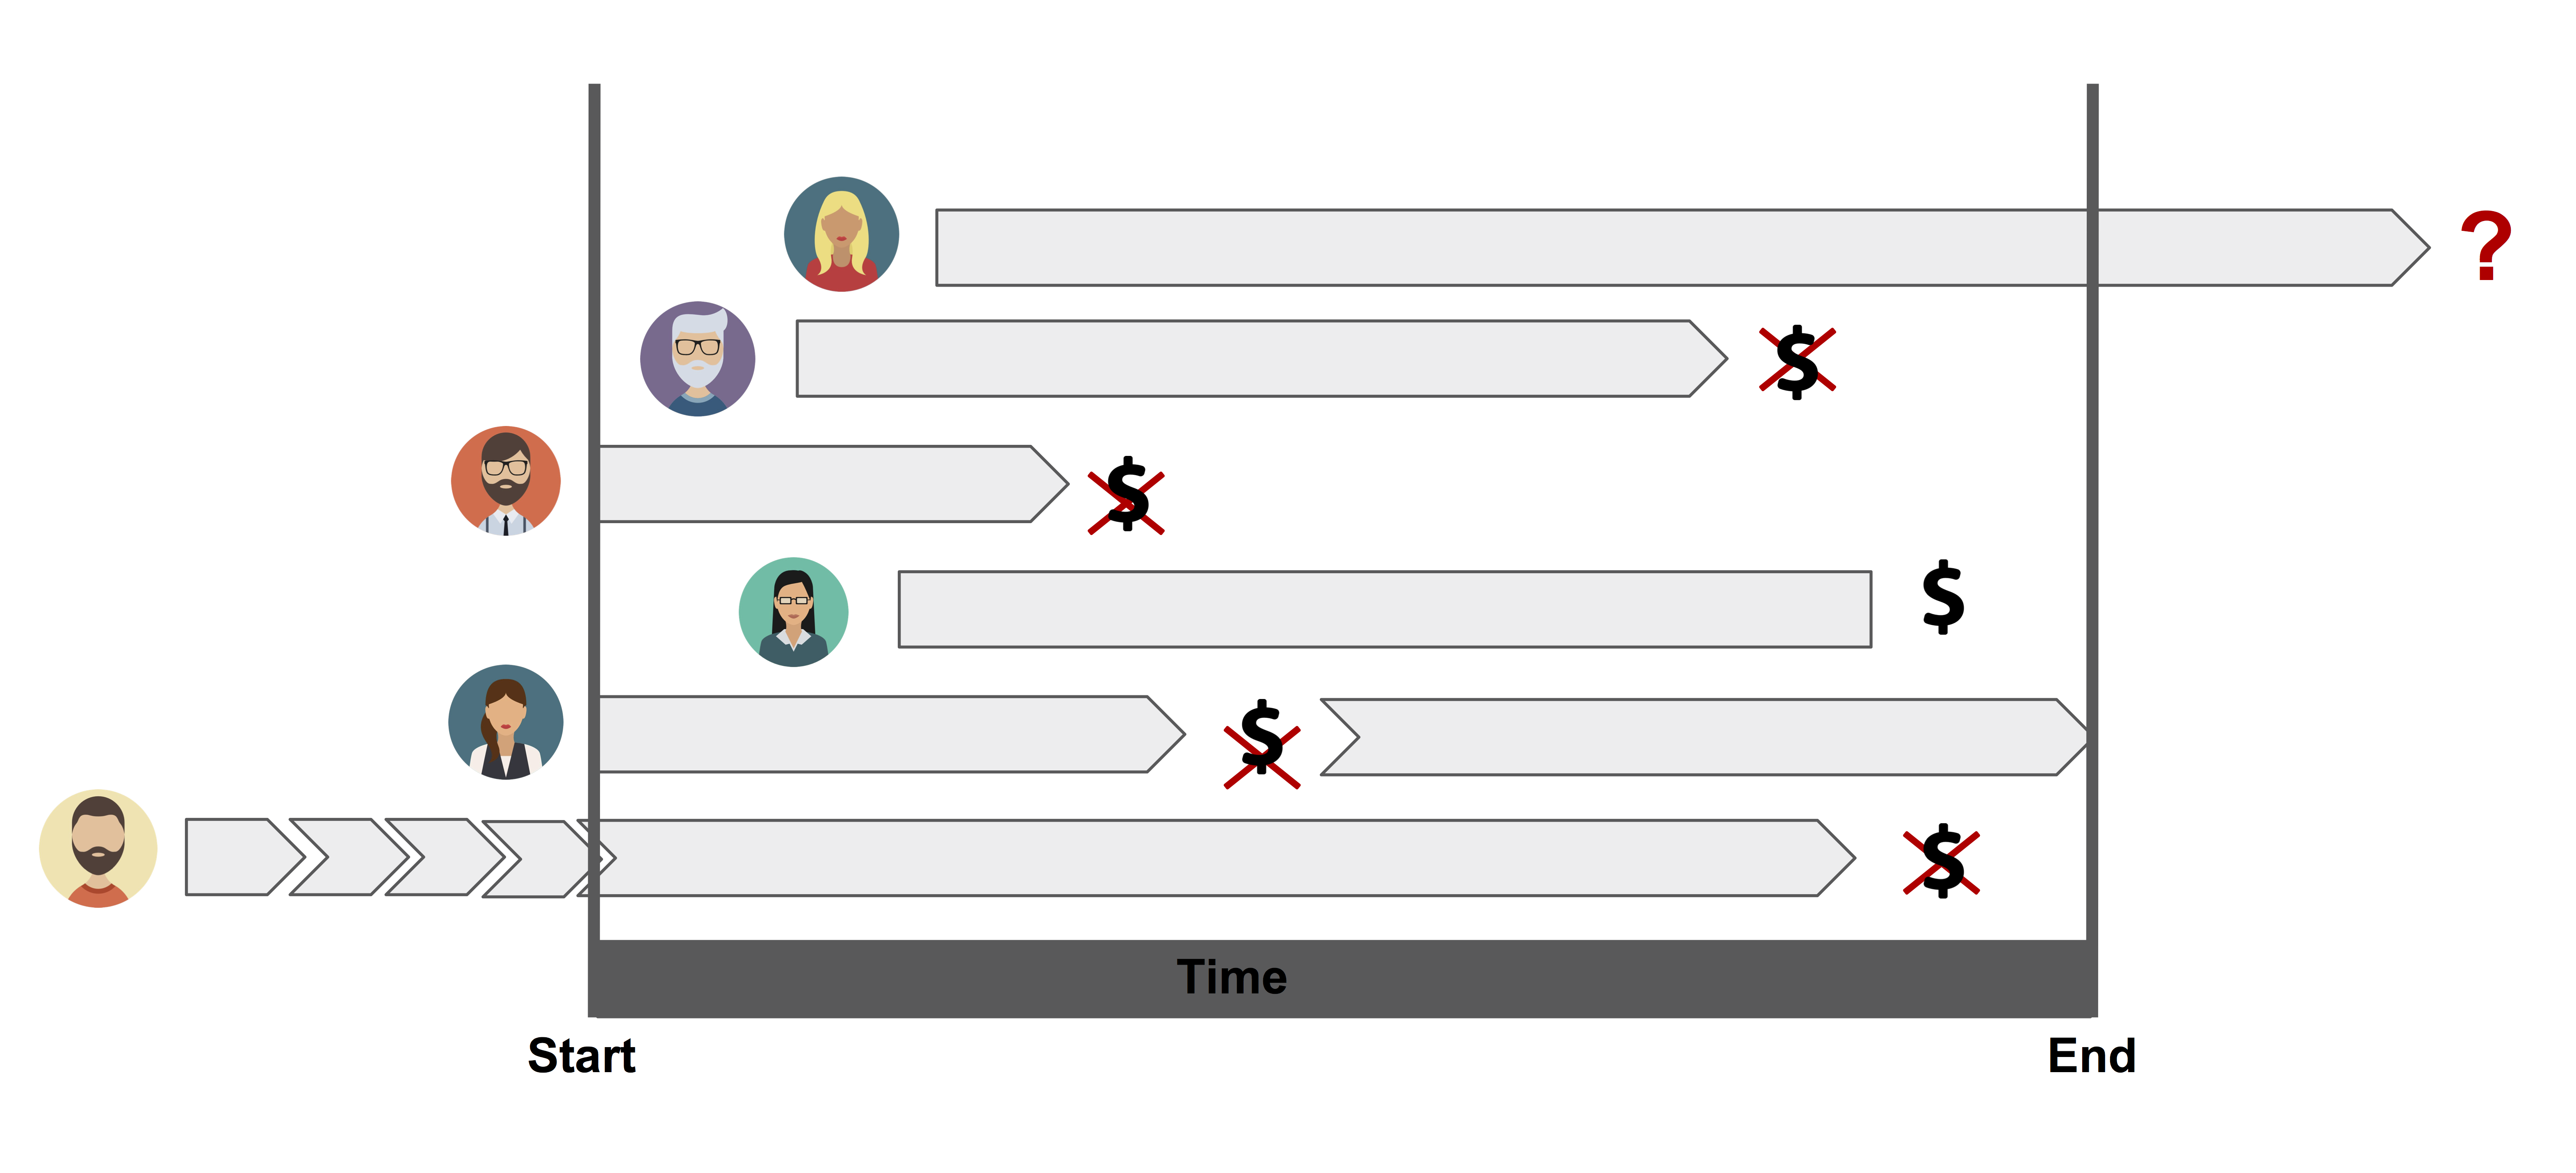
\includegraphics{images/saBBVA_censoring} 

}

\caption{Illustration of censoring.}\label{fig:censoring}
\end{figure}

\BeginKnitrBlock{rmdhint_sestelo}
It is important to highlight in this context (\textbf{time-to-default})
which situations we are going to considered as censoring. The bank has
special characteristics that are not seen in other applications.
\textbf{Censored cases} are considered to be loans that did \textbf{not
experience default} by the moment of data gathering. Additionally, early
\textbf{repayment} and \textbf{mature} cases (or complete, those ones
who reach their predefined end date before the moment of data gathering)
are also marked censored.
\EndKnitrBlock{rmdhint_sestelo}

Another classification:

\begin{itemize}
\item
  \textbf{Random type I censoring}: Also known as \emph{Generalized Type
  I Censoring}. When individuals enter the study at different times and
  the terminal point of the study is predetermined by the investigator,
  so that the censoring times are known when an individual is entered
  into the study.
\item
  \textbf{Type II censoring}: The study continues until the failure of
  the first \(r\) individuals, where \(r\) is some predetermined integer
  (\(r<n\)). All subjects are put on test at the same time, and the test
  is terminated when \(r\) of the \(n\) subjects have ``failed''.
\end{itemize}

\section{Some notation}\label{intro-notation}

We are now ready to introduce \textbf{basic mathematical terminology}
and \textbf{notation} for survival analysis.

Let \(T\) the random variable that denotes the survival time, i.e., the
time to an event. Since \(T\) denotes time, its possible values include
all nonnegative numbers; that is, \(T\) can be any number equal to or
greater than zero. Furthermore, \(t\) will be any specific value of
interest for the random variable \(T\).

Additionally, when each subject has a random right censoring time
\(C_i\) that is independent of their failure time \(T_i\), the data is
represented by \((Y_i, \Delta_i)\) where \(Y_i = \min(T_i, C_i)\) and
\(\Delta_i = I(T_i \le C_i)\), this \(\Delta\) define a \((0,1)\) random
variable indicating either failure or censorship. That is,
\(\Delta = 1\) for failure if the event occurs during the study period,
or \(\Delta = 0\) if the survival time is censored by the end of the
study period.

\section{Survival/hazard functions}\label{intro-functions}

Assuming that \(T\) is a continuous non-negative random variable which
denote the time-to-event. There is a certain probability that an
individual will have an event at exactly time \(t\). For example, about
human longevity, human beings have a certain probability of dying at
ages \(2\), \(20\), \(80\), and \(140\), that could be: \(P(T=2)\),
\(P(T=20)\), \(P(T=80)\) and \(P(T=140)\).

Similarly, human beings have a certain probability of being alive at
those same ages: \(P(T>2)\), \(P(T>20)\), \(P(T>80)\), and \(P(T>140)\).

Here an example with same real data \footnote{Data from \emph{The Human
  Mortality Database} at \url{http://www.mortality.org}.}:

\begin{Shaded}
\begin{Highlighting}[]
\NormalTok{data <-}\StringTok{ }\KeywordTok{read.table}\NormalTok{(}\StringTok{"data/deaths_esp.txt"}\NormalTok{, }\DataTypeTok{header =} \OtherTok{TRUE}\NormalTok{, }\DataTypeTok{sep =} \StringTok{""}\NormalTok{)}
\NormalTok{data <-}\StringTok{ }\NormalTok{data[}\OperatorTok{!}\NormalTok{data}\OperatorTok{$}\NormalTok{Age }\OperatorTok{==}\StringTok{ "110+"}\NormalTok{, ] }\CommentTok{# to avoid errors}
\NormalTok{data}\OperatorTok{$}\NormalTok{Age_cut <-}\StringTok{ }\KeywordTok{cut}\NormalTok{(}\KeywordTok{as.numeric}\NormalTok{(}\KeywordTok{as.character}\NormalTok{(data}\OperatorTok{$}\NormalTok{Age)), }
                 \DataTypeTok{breaks =}  \KeywordTok{seq}\NormalTok{(}\DecValTok{0}\NormalTok{,}\DecValTok{110}\NormalTok{, }\DecValTok{10}\NormalTok{), }\DataTypeTok{right =} \OtherTok{FALSE}\NormalTok{)}

\NormalTok{by_age <-}\StringTok{ }\NormalTok{data }\OperatorTok
\StringTok{  }\KeywordTok{group_by}\NormalTok{(Age_cut)  }\OperatorTok
\StringTok{  }\KeywordTok{summarise}\NormalTok{ (}\DataTypeTok{sum_deaths =} \KeywordTok{sum}\NormalTok{(Total, }\DataTypeTok{na.rm =} \OtherTok{TRUE}\NormalTok{))}

\KeywordTok{barplot}\NormalTok{(by_age}\OperatorTok{$}\NormalTok{sum_deaths}\OperatorTok{/}\KeywordTok{sum}\NormalTok{(data}\OperatorTok{$}\NormalTok{Total), }\DataTypeTok{names.arg =}\NormalTok{ by_age}\OperatorTok{$}\NormalTok{Age_cut, }\DataTypeTok{ylab=} \StringTok{"Relative frequency"}\NormalTok{) }
\end{Highlighting}
\end{Shaded}

\begin{figure}
\centering
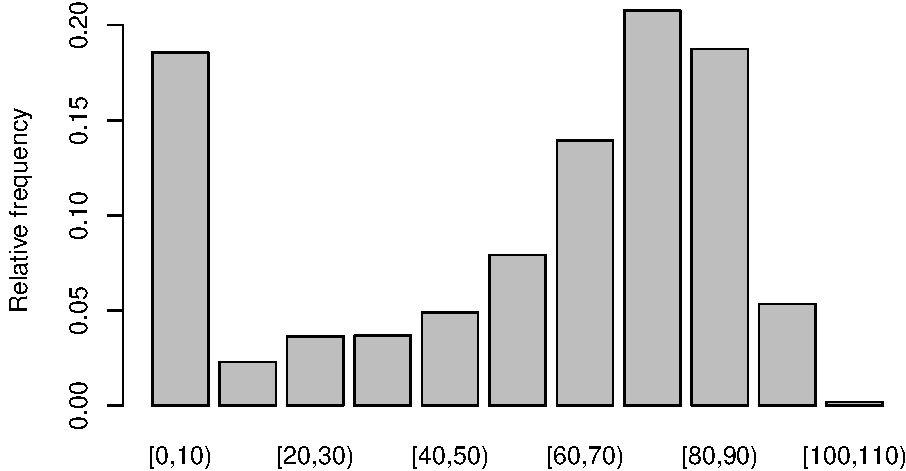
\includegraphics{bookdown_files/figure-latex/unnamed-chunk-6-1.pdf}
\caption{\label{fig:unnamed-chunk-6}Relative frequiencies for grouped ages.}
\end{figure}

In the case of human longevity, the probability of death is higher at
the beginning and end of life (in Spain). Therefore, \(T\) is unlikely
to follow a normal distribution. We can see a higher chance of dying
(the event of interest) in their 70's and 80's and smaller chance of
dying in their 100's and 110's, because few people make it long enough
to die at these age.

The function that gives the probability of the failure time occurring at
exactly time \(t\) is the \textbf{density function \(f(t)\)} \footnote{The
  probability mass function is a function that gives the probability
  that a discrete random variable is exactly equal to some value.}

\[
f(t) = \displaystyle{lim_{\Delta_t \to 0}} \frac{P(t \le T < t + \Delta t)}{\Delta t}
\] and the function that gives the probability of the failure time occur
before or exactly at time \(t\) is the \textbf{cumulative distribution
function \(F(t)\)}

\[
F(t) = P(T \le t) = \int_{0}^{t} f(u) du.
\]

Note that \(F(t)\) is more interesting than \(f(t)\)\ldots{} And why?
Well, as we said, the main goal of survival analysis is to estimate and
compare survival experiences of different groups and the survival
experience is described by the \textbf{survival function \(S(t)\)}

\[
S(t) = P(T > t) = 1 - F(t)
\]

The survival function gives the probability that a person survives
longer than some specified time \(t\): that is, \(S(t)\) gives the
probability that the random variable \(T\) exceeds the specified time
\(t\). And here, some important characteristics:

\begin{itemize}
\item
  It is nonincreasing; that is, it heads downward as \(t\) increases.
\item
  At time \(t = 0\), \(S(t) = S(0)= 1\); that is, at the start of the
  study, since no one has gotten the event yet, the probability of
  surviving past time zero is one.
\item
  At time \(t = \inf\), \(S(t) = S(\inf) = 0\); that is, theoretically,
  if the study period increased without limit, eventually nobody would
  survive, so the survival curve must eventually fall to zero.
\end{itemize}

\begin{Shaded}
\begin{Highlighting}[]
\NormalTok{t <-}\StringTok{ }\KeywordTok{seq}\NormalTok{(}\DecValTok{0}\NormalTok{, }\DecValTok{110}\NormalTok{, }\DecValTok{1}\NormalTok{)}
\NormalTok{tdf <-}\StringTok{ }\KeywordTok{pweibull}\NormalTok{(t, }\DataTypeTok{scale =} \DecValTok{80}\NormalTok{, }\DataTypeTok{shape =} \DecValTok{5}\NormalTok{) }\CommentTok{# weibull dist}

\NormalTok{d <-}\StringTok{ }\NormalTok{reshape2}\OperatorTok{::}\KeywordTok{melt}\NormalTok{(}\KeywordTok{data.frame}\NormalTok{(}\DataTypeTok{x =}\NormalTok{ t, }\DataTypeTok{dist =}\NormalTok{ tdf, }\DataTypeTok{surv =} \DecValTok{1} \OperatorTok{-}\StringTok{ }\NormalTok{tdf), }\DataTypeTok{id =} \StringTok{"x"}\NormalTok{)}
\KeywordTok{qplot}\NormalTok{(}\DataTypeTok{x =}\NormalTok{ x, }\DataTypeTok{y =}\NormalTok{ value, }\DataTypeTok{col =}\NormalTok{ variable, }\DataTypeTok{data =}\NormalTok{ d, }\DataTypeTok{geom =} \StringTok{"line"}\NormalTok{, }
      \DataTypeTok{ylab =} \StringTok{"probability"}\NormalTok{, }\DataTypeTok{xlab =} \StringTok{"t"}\NormalTok{) }\OperatorTok{+}\StringTok{ }
\StringTok{  }\KeywordTok{scale_colour_discrete}\NormalTok{(}\DataTypeTok{labels=} \KeywordTok{c}\NormalTok{(}\StringTok{"F(t)"}\NormalTok{, }\StringTok{"S(t)"}\NormalTok{), }\DataTypeTok{name =} \StringTok{""}\NormalTok{) }
\end{Highlighting}
\end{Shaded}

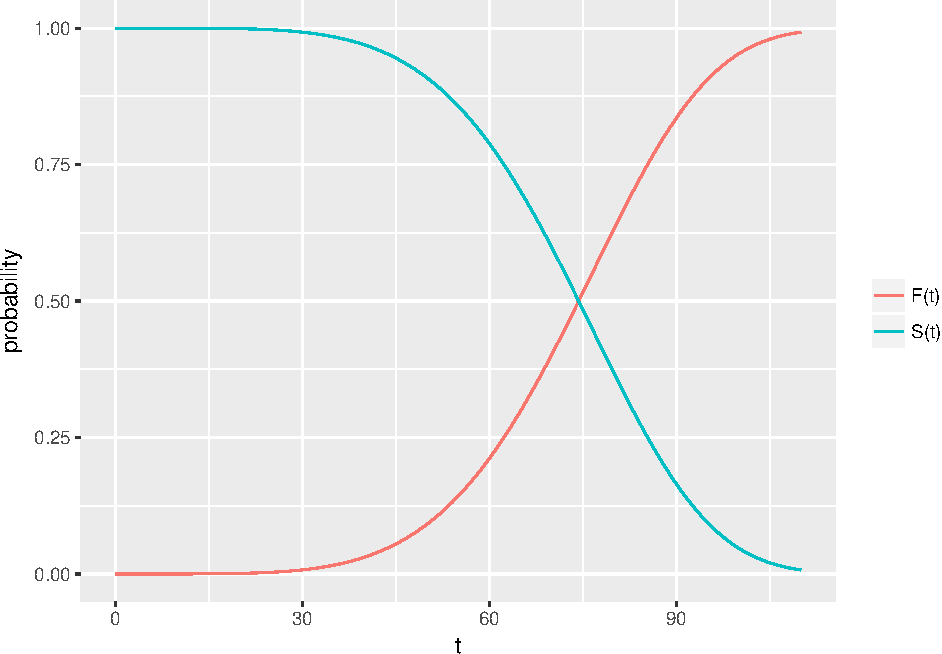
\includegraphics{bookdown_files/figure-latex/unnamed-chunk-7-1.pdf}

Note that these are theoretical properties of survival curves. In
practice, when using actual data, we usually obtain graphs that are step
functions, rather than smooth curves. Moreover, because the study period
is never infinite in length and there may be competing risks for
failure, it is possible that not everyone studied gets the event. The
estimated survival function, \(\hat{S}(t)\) thus may not go all the way
down to zero at the end of the study.

\begin{Shaded}
\begin{Highlighting}[]
\NormalTok{by_age <-}\StringTok{ }\NormalTok{data }\OperatorTok
\StringTok{  }\KeywordTok{group_by}\NormalTok{(Age)  }\OperatorTok
\StringTok{  }\KeywordTok{summarise}\NormalTok{ (}\DataTypeTok{sum_deaths =} \KeywordTok{sum}\NormalTok{(Total, }\DataTypeTok{na.rm =}\NormalTok{ T))}
\NormalTok{t <-}\StringTok{ }\KeywordTok{rep}\NormalTok{(}\KeywordTok{as.numeric}\NormalTok{(}\KeywordTok{as.character}\NormalTok{(by_age}\OperatorTok{$}\NormalTok{Age)), by_age}\OperatorTok{$}\NormalTok{sum_deaths) }\CommentTok{# real times}

\NormalTok{aux <-}\StringTok{ }\KeywordTok{ecdf}\NormalTok{(t)}
\NormalTok{x <-}\StringTok{ }\KeywordTok{seq}\NormalTok{(}\DecValTok{0}\NormalTok{, }\DecValTok{110}\NormalTok{, }\DecValTok{1}\NormalTok{)}
\NormalTok{edf <-}\StringTok{ }\KeywordTok{aux}\NormalTok{(x) }\CommentTok{# evaluating the ecdf in some points}
\NormalTok{esf <-}\StringTok{ }\DecValTok{1}\OperatorTok{-}\StringTok{ }\NormalTok{edf}

\NormalTok{d <-}\StringTok{ }\NormalTok{reshape2}\OperatorTok{::}\KeywordTok{melt}\NormalTok{(}\KeywordTok{data.frame}\NormalTok{(}\DataTypeTok{x =}\NormalTok{ x, }\DataTypeTok{dist =}\NormalTok{ edf, }\DataTypeTok{surv =}\NormalTok{ esf), }\DataTypeTok{id =} \StringTok{"x"}\NormalTok{)}
\KeywordTok{qplot}\NormalTok{(}\DataTypeTok{x =}\NormalTok{ x, }\DataTypeTok{y =}\NormalTok{ value, }\DataTypeTok{col =}\NormalTok{ variable, }\DataTypeTok{data =}\NormalTok{ d, }\DataTypeTok{geom =} \StringTok{"step"}\NormalTok{, }
      \DataTypeTok{ylab =} \StringTok{"Probability"}\NormalTok{, }\DataTypeTok{xlab =} \StringTok{"t"}\NormalTok{) }\OperatorTok{+}\StringTok{ }\KeywordTok{scale_colour_discrete}\NormalTok{(}\DataTypeTok{labels =} \KeywordTok{c}\NormalTok{(}\StringTok{"F(t)"}\NormalTok{, }\StringTok{"S(t)"}\NormalTok{), }\DataTypeTok{name =} \StringTok{""}\NormalTok{)}
\end{Highlighting}
\end{Shaded}

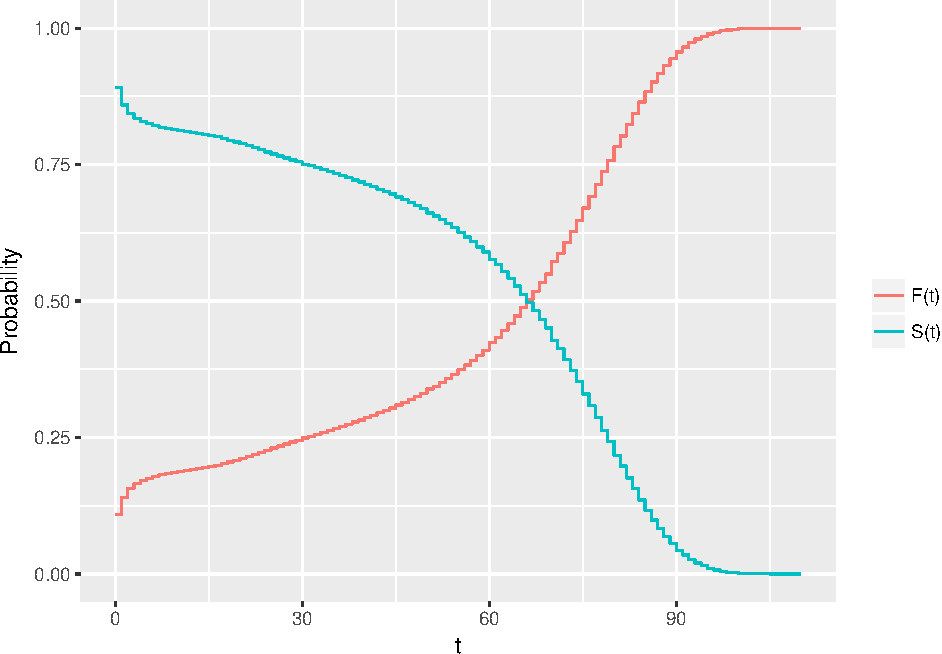
\includegraphics{bookdown_files/figure-latex/unnamed-chunk-8-1.pdf}

The \textbf{hazard function \(h(t)\)}, is given by the formula:

\[
h(t) = \displaystyle{lim_{\Delta_t \to 0}} \frac{P(t \le T < t + \Delta t | T \ge t)}{\Delta t}
\] This mathematical formula is difficult to explain in practical terms.
We could say that the hazard function is the probability that if you
survive to time \(t\), you will experience the event in the next
instant, or in other words, the hazard function gives the instantaneous
potential per unit time for the event to occur, given that the
individual has survived up to time \(t\). Because of the given sign
here, the hazard function is sometimes called a \textbf{conditional
failure rate}.

Note that, in contrast to the \textbf{survival function}, which focuses
on \textbf{not failing}, the \textbf{hazard function} focuses on
\textbf{failing}, that is, on the event occurring. Thus, in some sense,
the hazard function can be considered as giving the opposite side of the
information given by the survivor function.

Additionally, in contrast to a survival function, the graph of \(h(t)\)
does not have to start at one and go down to zero, but rather can start
anywhere and go up and down in any direction over time. In particular,
for a specified value of \(t\), the hazard function \(h(t)\) has the
following characteristics:

\begin{itemize}
\item
  It is always nonnegative, that is, equal to or greater than zero.
\item
  It has no upper bound.
\end{itemize}

Finally note that the hazard function can be expressed as the
probability density function divided by the survival function,
\(h(t) = \frac{f(t)}{S(t)}\):

\[
P(t \le T \lt t + dt | T \ge t) = \frac{P(t \le T \lt t + dt, T \ge t)}{P(T \ge t)} = \frac{P(t \le T \lt t + dt)}{P(T \ge t)}
\]

\begin{Shaded}
\begin{Highlighting}[]
\NormalTok{h <-}\StringTok{ }\KeywordTok{hist}\NormalTok{(t, }\DataTypeTok{plot =} \OtherTok{FALSE}\NormalTok{)}
\NormalTok{x <-}\StringTok{ }\NormalTok{h}\OperatorTok{$}\NormalTok{mids}
\NormalTok{dens <-}\StringTok{ }\NormalTok{h}\OperatorTok{$}\NormalTok{density}
\NormalTok{surv <-}\StringTok{ }\DecValTok{1} \OperatorTok{-}\StringTok{ }\KeywordTok{aux}\NormalTok{(x)}
\NormalTok{hazard <-}\StringTok{ }\NormalTok{dens}\OperatorTok{/}\NormalTok{surv}
\KeywordTok{qplot}\NormalTok{(}\DataTypeTok{x =}\NormalTok{ x, }\DataTypeTok{y =}\NormalTok{ hazard, }\DataTypeTok{geom =} \StringTok{"line"}\NormalTok{, }\DataTypeTok{ylab =} \StringTok{"Conditional probability of death"}\NormalTok{,}
      \DataTypeTok{xlab =} \StringTok{"Age"}\NormalTok{)}
\end{Highlighting}
\end{Shaded}

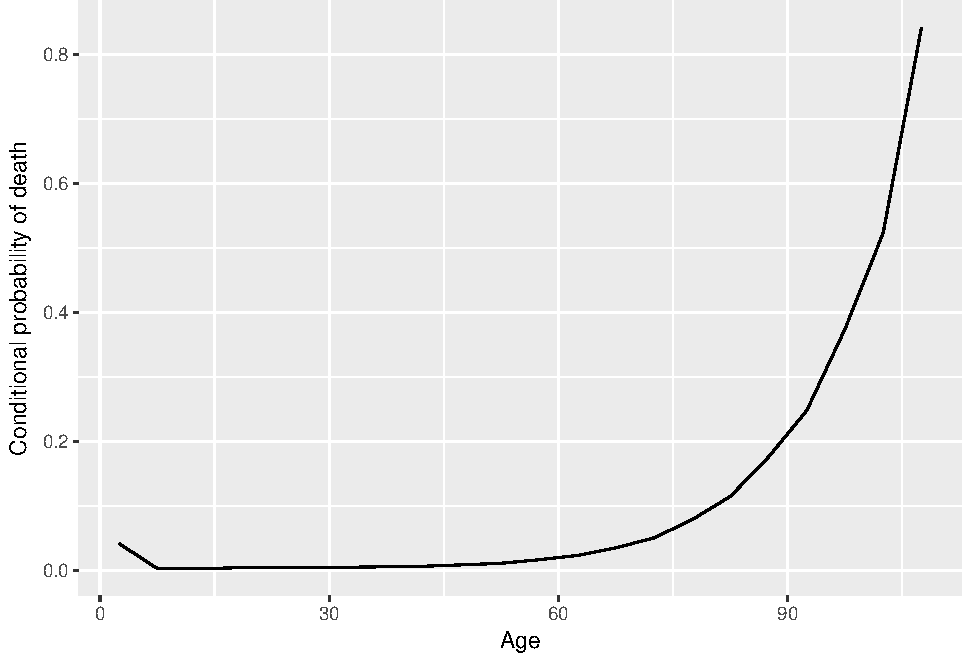
\includegraphics{bookdown_files/figure-latex/unnamed-chunk-9-1.pdf}

In some cases it can be more interesting to present the cumulative
hazard. It will be \(H(t) = \int_{0}^{t} h(u) du\).

\BeginKnitrBlock{rmdhint_sestelo}
\textbf{Hazard vs.~density function}

According to the human longevity study, note that when you are born, you
have a certain probability of dying at any age, that will be
\(P(T = t)\), i.e.~the density function. A woman born today has, say, a
1\% chance of dying at 80 years. However, as you survive for a while,
your probabilities keep changing, and these new conditional
probabilities are given by the hazard function. In such case, we have a
woman who is 79 today and has, say, a 7\% chance of dying at 80 years.
\EndKnitrBlock{rmdhint_sestelo}

\section{Relation between functions}\label{relation-between-functions}

For \textbf{parametric} survival models, time is assumed to follow some
well-known distribution whose probability density function \(f(t)\) can
be expressed in terms of unknown parameters. Once a probability density
function is specified for survival time, the corresponding survival and
hazard functions can be determined.

For example, the \textbf{survival function} can be ascertained from the
\textbf{probability density function} by integrating over the
probability density function from time \(t\) to infinity, or by
calculating the difference between one and the \textbf{cumulative
distribution function} \(F(t)\). The \textbf{hazard} can then be found
by dividing the negative derivative of the survival function by the
survival function. Note that the functions \(f(t)\), \(F(t)\), \(h(t)\),
and \(H(t)\) are all related.

\begin{enumerate}
\item
  Assume that \(T\) is \textbf{non-negative and continuos}:

  \begin{itemize}
  \item
    Probability density function:

    \begin{itemize}
    \tightlist
    \item
      \(f(t) = F'(t) = \frac{dF(t)}{dt}\)
    \end{itemize}
  \item
    Cumulative distribution function:

    \begin{itemize}
    \tightlist
    \item
      \(F(t) = P(T \le t) = \int_0^t{f(u)}{du}\)
    \end{itemize}
  \item
    Survival function

    \begin{itemize}
    \item
      \(S(t) = 1 - F(t)\)
    \item
      \(S(t) = P(T > t) = \int_t^{+\infty}{f(u)}{du}\)
    \item
      \(S(t) = exp \left( - \int_0^t h(u) du \right)\)
    \item
      \(S(t) = \exp(-H(t))\)
    \end{itemize}
  \item
    Hazard function

    \begin{itemize}
    \tightlist
    \item
      \(h(t) = \frac{ f(t)}{S(t)}= \frac{ -d[S(t)]/dt}{S(t)}\)
    \end{itemize}
  \item
    Cumulative hazard function

    \begin{itemize}
    \tightlist
    \item
      \(H(t) = \int_0^t h(u) du\)
    \end{itemize}
  \end{itemize}
\end{enumerate}

\begin{enumerate}
\item
  Assume that \(T\) is \textbf{non-negative and discrete},

  \begin{itemize}
  \tightlist
  \item
    Probability mass function:

    \begin{itemize}
    \tightlist
    \item
      \(p(t_i) = P(T = t_i)\)
    \item
      \(p(t_i) = S(t_{i-1}) - S(t_i)\)
    \item
      \(p(t_i) = F(t_i) - F(t_{i-1})\)
    \end{itemize}
  \item
    Cumulative distribution function:

    \begin{itemize}
    \tightlist
    \item
      \(F(t) = P(T \le t) = \sum_{t_i \le t}{p(t_i)}\)
    \end{itemize}
  \item
    Survival function

    \begin{itemize}
    \tightlist
    \item
      \(S(t) = \prod_{t_i \le t} \left( 1 - h(t_i) \right)\)
    \end{itemize}
  \item
    Hazard function

    \begin{itemize}
    \tightlist
    \item
      \(h(t) = \frac{ p(t_i)}{S(t_{i-1})}= \frac{ -d[S(t)]/dt}{S(t)}\)
    \item
      \(h(t) = 1- \frac{ S(t_i)}{S(t_{i-1})}\)
    \end{itemize}
  \item
    Cumulative hazard function

    \begin{itemize}
    \tightlist
    \item
      \(H(t) = \sum_{t_i \le t} h(t_i)\)
    \end{itemize}
  \end{itemize}
\end{enumerate}

\section{Some common distributions}\label{intro-distri}

\begin{longtable}[]{@{}lll@{}}
\toprule
\begin{minipage}[b]{0.24\columnwidth}\raggedright\strut
Definition\strut
\end{minipage} & \begin{minipage}[b]{0.28\columnwidth}\raggedright\strut
Functions\strut
\end{minipage} & \begin{minipage}[b]{0.39\columnwidth}\raggedright\strut
Measures\strut
\end{minipage}\tabularnewline
\midrule
\endhead
\begin{minipage}[t]{0.32\columnwidth}\raggedright\strut
\textbf{Exponential}

\(T\sim Exp(  \lambda)\)\strut
\end{minipage} & \begin{minipage}[t]{0.32\columnwidth}\raggedright\strut
\begin{itemize}
\item
  \(f(t)=\lambda  exp(-\lambda t)\) where \(t \ge 0 and  \lambda > 0\)
\item
  \(F(t)=1-exp(-\lambda  t)\)
\item
  \(S(t)=exp(-\lambda  t)\)
\item
  \(h(t) = \lambda\)
\item
  \(H(t) = \lambda t\)
\end{itemize}\strut
\end{minipage} & \begin{minipage}[t]{0.32\columnwidth}\raggedright\strut
\(E(T)=\int_0^{+\infty}uf(u) du= \frac{1}{\lambda}\)

\(Var(T)=E(T^2)-E(T)^2 =  \ldots = \frac{1}{\lambda^2}\)\strut
\end{minipage}\tabularnewline
\begin{minipage}[t]{0.32\columnwidth}\raggedright\strut
\textbf{Weibull}

\(T\sim Weib(a,b)\) with \(a\) shape and \(b\) scale\strut
\end{minipage} & \begin{minipage}[t]{0.32\columnwidth}\raggedright\strut
\begin{itemize}
\item
  \(f(t)=\frac{a}{b}  (\frac{t}{b})^{a-1}  exp^{-\left(\frac{t}  {b} \right)^a}\)
  where \(t\ge 0\) and \(a,b> 0\)
\item
  \(F(t)= 1-exp^{-  \left(\frac{t}{b}  \right)^a}\)
\item
  \(S(t)=exp^{-\left( \frac{t}{b}  \right)^a}\)
\item
  \(h(t)=ab^{-a}t^{a-1}\)
\item
  \(H(t)=(\frac{t}  {b})^a\)
\end{itemize}\strut
\end{minipage} & \begin{minipage}[t]{0.32\columnwidth}\raggedright\strut
\(E(T)=b\Gamma \left(1+  \frac{1}{a}\right)\)

\(Var(T) = b^2 \Gamma \left(1+  \frac{2}{a}\right) - b^2  \left [ \Gamma \left(1+  \frac{1}{a}\right)\right]^2\)

where, \(\Gamma(k)\) is the gamma function.

\(\Gamma (k) = \int_0^{+\infty} u^{k-1} exp^{-u}du\)\strut
\end{minipage}\tabularnewline
\bottomrule
\end{longtable}

There are other distributions such as Log-Normal, Log-Logistic, Pareto,
Rayleigh, Gomptertz, or even more. For more details see
\url{http://data.princeton.edu/pop509/ParametricSurvival.pdf}.

\chapter{Kaplan Meier estimator}\label{km}

Once we have explained what is the survival curve and other introductory
questions, we move on the estimation. Note that we can estimate the
survival (or hazard) function in two ways:

\begin{itemize}
\item
  by specifying a \textbf{parametric} model for \(\lambda(t)\) based on
  a particular density function \(f(t)\) (parametric estimation)
\item
  by developing an \textbf{empirical} estimate of the survival function
  (i.e., \textbf{nonparametric} estimation)
\end{itemize}

This Chapter describes how to plot and interpret survival data using the
Kaplan-Meier (KM) estimator (nonparametric) and how to test whether or
not two or more KM curves are equivalent using the log--rank test.
Alternative tests to the log--rank test are also described. Furthermore,
methods for computing \((1-\alpha)\)\% confidence intervals for a KM
curve are afforded.

\section{Estimating survival by means of the Kaplan Meier
estimator}\label{estimating-survival-by-means-of-the-kaplan-meier-estimator}

If there are no censored observations in a sample of dimension \(n\),
the most natural estimator for survival is the \textbf{empirical
estimator}, given by

\[
\hat S(t) = P(T \gt t) = \frac{1}{n} \sum_{i=1}^{n} I(t_i \gt t)
\] that is, the proportion of observations with failure times greater
than \(t\).

\begin{Shaded}
\begin{Highlighting}[]
\NormalTok{x <-}\StringTok{ }\KeywordTok{c}\NormalTok{(}\DecValTok{1}\NormalTok{, }\DecValTok{1}\NormalTok{, }\DecValTok{2}\NormalTok{, }\DecValTok{2}\NormalTok{, }\DecValTok{3}\NormalTok{, }\DecValTok{4}\NormalTok{, }\DecValTok{4}\NormalTok{, }\DecValTok{5}\NormalTok{, }\DecValTok{5}\NormalTok{, }\DecValTok{8}\NormalTok{, }\DecValTok{8}\NormalTok{, }\DecValTok{8}\NormalTok{, }\DecValTok{8}\NormalTok{, }\DecValTok{11}\NormalTok{, }\DecValTok{11}\NormalTok{, }\DecValTok{12}\NormalTok{, }\DecValTok{12}\NormalTok{, }\DecValTok{15}\NormalTok{, }\DecValTok{17}\NormalTok{, }\DecValTok{22}\NormalTok{, }\DecValTok{23}\NormalTok{)}
\KeywordTok{sum}\NormalTok{(x }\OperatorTok{>}\StringTok{ }\DecValTok{8}\OperatorTok{/}\KeywordTok{length}\NormalTok{(n)) }\CommentTok{# hat S(8) }
\NormalTok{## [1] 8}
\KeywordTok{sum}\NormalTok{(x }\OperatorTok{>}\StringTok{ }\DecValTok{12}\OperatorTok{/}\KeywordTok{length}\NormalTok{(n)) }\CommentTok{# hat S(12) }
\NormalTok{## [1] 4}
\end{Highlighting}
\end{Shaded}

Another option for estimating survival could be to use the hazard:

\[
\hat S(t) = \prod_{k = 1}^{t-1} \bigg [ 1- \hat \lambda(k)\bigg] \quad {\text{where}} \quad  \hat \lambda(t) = \frac{\sum_{i=1}^{n} I(Y_i = t)}{\sum_{i=1}^{n} I (Y_i \ge t)} 
\]

Note that \(\hat \lambda(t)\) is obtained as the number of individuals
that die at time \(t\) divided by the number of individuals that survive
to \(t\), the number of individuals at risk at time \(t\) (using the
death as event).

However, alternative methods are necessary to incorporate censoring
(censored times are different than event times).

\begin{Shaded}
\begin{Highlighting}[]
\CommentTok{#  preprocesing data}

\KeywordTok{head}\NormalTok{(loan)[, }\KeywordTok{c}\NormalTok{(}\DecValTok{51}\NormalTok{, }\DecValTok{65}\NormalTok{, }\DecValTok{6}\NormalTok{, }\DecValTok{7}\NormalTok{, }\DecValTok{19}\NormalTok{, }\DecValTok{18}\NormalTok{, }\DecValTok{50}\NormalTok{)]}
\NormalTok{##                   LoanKey LoanOriginationDate LoanStatus}
\NormalTok{## 1 E33A3400205839220442E84 2007-09-12 00:00:00  Completed}
\NormalTok{## 2 9E3B37071505919926B1D82 2014-03-03 00:00:00    Current}
\NormalTok{## 3 6954337960046817851BCB2 2007-01-17 00:00:00  Completed}
\NormalTok{## 4 A0393664465886295619C51 2012-11-01 00:00:00    Current}
\NormalTok{## 5 A180369302188889200689E 2013-09-20 00:00:00    Current}
\NormalTok{## 6 C3D63702273952547E79520 2013-12-24 00:00:00    Current}
\NormalTok{##            ClosedDate    Occupation BorrowerState StatedMonthlyIncome}
\NormalTok{## 1 2009-08-14 00:00:00         Other            CO            3083.333}
\NormalTok{## 2                      Professional            CO            6125.000}
\NormalTok{## 3 2009-12-17 00:00:00         Other            GA            2083.333}
\NormalTok{## 4                     Skilled Labor            GA            2875.000}
\NormalTok{## 5                         Executive            MN            9583.333}
\NormalTok{## 6                      Professional            NM            8333.333}
\KeywordTok{table}\NormalTok{(loan}\OperatorTok{$}\NormalTok{LoanStatus)}
\NormalTok{## }
\NormalTok{##              Cancelled             Chargedoff              Completed }
\NormalTok{##                      5                  11992                  38074 }
\NormalTok{##                Current              Defaulted FinalPaymentInProgress }
\NormalTok{##                  56576                   5018                    205 }
\NormalTok{##   Past Due (>120 days)   Past Due (1-15 days)  Past Due (16-30 days) }
\NormalTok{##                     16                    806                    265 }
\NormalTok{##  Past Due (31-60 days)  Past Due (61-90 days) Past Due (91-120 days) }
\NormalTok{##                    363                    313                    304}

\CommentTok{# removing duplicates}
\NormalTok{loan_nd <-}\StringTok{ }\NormalTok{loan[}\KeywordTok{unique}\NormalTok{(loan}\OperatorTok{$}\NormalTok{LoanKey), ] }

\CommentTok{# removing LoanStatus no needed }
\NormalTok{sel_status  <-}\StringTok{ }\NormalTok{loan_nd}\OperatorTok{$}\NormalTok{LoanStatus }\OperatorTok\StringTok{ }\KeywordTok{c}\NormalTok{(}\StringTok{"Completed"}\NormalTok{, }\StringTok{"Current"}\NormalTok{, }
                                          \StringTok{"ChargedOff"}\NormalTok{, }\StringTok{"Defaulted"}\NormalTok{, }
                                          \StringTok{"Cancelled"}\NormalTok{)}
\NormalTok{loan_filtered <-}\StringTok{ }\NormalTok{loan_nd[sel_status, ]}

\CommentTok{# creating status variable for censoring}
\NormalTok{loan_filtered}\OperatorTok{$}\NormalTok{status <-}\StringTok{ }\KeywordTok{ifelse}\NormalTok{(}
\NormalTok{  loan_filtered}\OperatorTok{$}\NormalTok{LoanStatus }\OperatorTok{==}\StringTok{ "Defaulted"} \OperatorTok{|}
\StringTok{    }\NormalTok{loan_filtered}\OperatorTok{$}\NormalTok{LoanStatus }\OperatorTok{==}\StringTok{ "Chargedoff"}\NormalTok{,  }\DecValTok{1}\NormalTok{, }\DecValTok{0}\NormalTok{)}

\CommentTok{# adding the final date to "current" status}
\KeywordTok{head}\NormalTok{(}\KeywordTok{levels}\NormalTok{(loan_filtered}\OperatorTok{$}\NormalTok{ClosedDate))}
\NormalTok{## [1] ""                    "2005-11-25 00:00:00" "2005-11-29 00:00:00"}
\NormalTok{## [4] "2005-11-30 00:00:00" "2005-12-08 00:00:00" "2005-12-28 00:00:00"}
\KeywordTok{levels}\NormalTok{(loan_filtered}\OperatorTok{$}\NormalTok{ClosedDate)[}\DecValTok{1}\NormalTok{] <-}\StringTok{ "2014-11-03 00:00:00"}

\CommentTok{# creating the time-to-event variable}
\NormalTok{loan_filtered}\OperatorTok{$}\NormalTok{start <-}\StringTok{ }\KeywordTok{as.Date}\NormalTok{(loan_filtered}\OperatorTok{$}\NormalTok{LoanOriginationDate)}
\NormalTok{loan_filtered}\OperatorTok{$}\NormalTok{end <-}\StringTok{ }\KeywordTok{as.Date}\NormalTok{(loan_filtered}\OperatorTok{$}\NormalTok{ClosedDate)}
\NormalTok{loan_filtered}\OperatorTok{$}\NormalTok{time <-}\StringTok{ }\KeywordTok{as.numeric}\NormalTok{(}\KeywordTok{difftime}\NormalTok{(loan_filtered}\OperatorTok{$}\NormalTok{end, loan_filtered}\OperatorTok{$}\NormalTok{start, }\DataTypeTok{units =} \StringTok{"days"}\NormalTok{))}

\CommentTok{# there is an error in the data (time to event less than 0)}
\NormalTok{loan_filtered <-}\StringTok{ }\NormalTok{loan_filtered[}\OperatorTok{-}\NormalTok{loan_filtered}\OperatorTok{$}\NormalTok{time }\OperatorTok{<}\StringTok{ }\DecValTok{0}\NormalTok{, ]}

\CommentTok{# just considering a year of loans creation}
\NormalTok{ii <-}\StringTok{ }\KeywordTok{format}\NormalTok{(}\KeywordTok{as.Date}\NormalTok{(loan_filtered}\OperatorTok{$}\NormalTok{LoanOriginationDate),}\StringTok{'%Y'}\NormalTok{) }\OperatorTok\StringTok{ }
\StringTok{  }\KeywordTok{c}\NormalTok{(}\StringTok{"2006"}\NormalTok{)}
\NormalTok{loan_filtered <-}\StringTok{ }\NormalTok{loan_filtered[ii, ] }


\KeywordTok{dim}\NormalTok{(loan_filtered)}
\NormalTok{## [1] 4923   85}
\KeywordTok{head}\NormalTok{(loan_filtered)[, }\KeywordTok{c}\NormalTok{(}\DecValTok{51}\NormalTok{, }\DecValTok{65}\NormalTok{, }\DecValTok{6}\NormalTok{, }\DecValTok{7}\NormalTok{, }\DecValTok{19}\NormalTok{, }\DecValTok{18}\NormalTok{, }\DecValTok{50}\NormalTok{, }\DecValTok{83}\NormalTok{, }\DecValTok{84}\NormalTok{, }\DecValTok{85}\NormalTok{)]}
\NormalTok{##                       LoanKey LoanOriginationDate LoanStatus}
\NormalTok{## 55706 569F3376160094112B0CCBC 2006-12-07 00:00:00  Completed}
\NormalTok{## 5258  E3C433749566192177F6A25 2006-11-21 00:00:00  Completed}
\NormalTok{## 64330 3E5A33783711441966A924A 2006-12-29 00:00:00  Completed}
\NormalTok{## 1485  AC4533744391314602B8E3A 2006-12-07 00:00:00  Completed}
\NormalTok{## 22540 08B63364821540522E94FD2 2006-06-13 00:00:00  Completed}
\NormalTok{## 50637 31C9337247671326054DF29 2006-11-03 00:00:00  Completed}
\NormalTok{##                ClosedDate   Occupation BorrowerState StatedMonthlyIncome}
\NormalTok{## 55706 2009-07-27 00:00:00 Professional                          4534.250}
\NormalTok{## 5258  2008-07-03 00:00:00        Other                          3833.333}
\NormalTok{## 64330 2009-12-29 00:00:00       Doctor                         18083.333}
\NormalTok{## 1485  2008-11-21 00:00:00        Other            IN            4576.000}
\NormalTok{## 22540 2007-09-05 00:00:00                                       3458.333}
\NormalTok{## 50637 2009-11-03 00:00:00 Professional            IN           15666.667}
\NormalTok{##            start        end time}
\NormalTok{## 55706 2006-12-07 2009-07-27  963}
\NormalTok{## 5258  2006-11-21 2008-07-03  590}
\NormalTok{## 64330 2006-12-29 2009-12-29 1096}
\NormalTok{## 1485  2006-12-07 2008-11-21  715}
\NormalTok{## 22540 2006-06-13 2007-09-05  449}
\NormalTok{## 50637 2006-11-03 2009-11-03 1096}

\CommentTok{#------}



\CommentTok{# censoring status 0 = censored, 1 = no censored (default)}
\KeywordTok{table}\NormalTok{(loan_filtered}\OperatorTok{$}\NormalTok{status)}
\NormalTok{## }
\NormalTok{##    0    1 }
\NormalTok{## 3560 1363}
\KeywordTok{prop.table}\NormalTok{(}\KeywordTok{table}\NormalTok{(loan_filtered}\OperatorTok{$}\NormalTok{status))}
\NormalTok{## }
\NormalTok{##         0         1 }
\NormalTok{## 0.7231363 0.2768637}


\CommentTok{# median time until default (taking into account just no cendored data)}
\KeywordTok{median}\NormalTok{(loan_filtered}\OperatorTok{$}\NormalTok{time[loan_filtered}\OperatorTok{$}\NormalTok{status}\OperatorTok{==}\DecValTok{1}\NormalTok{])  }\CommentTok{# I'm underestimating}
\NormalTok{## [1] 333}


\CommentTok{# median time until default (with all data)}
\KeywordTok{mean}\NormalTok{(loan_filtered}\OperatorTok{$}\NormalTok{time)  }\CommentTok{# I'm underestimating the median survival too }
\NormalTok{## [1] 633.4331}
\CommentTok{# (in censored times, the real time is bigger)}
\end{Highlighting}
\end{Shaded}

\citet{KM58} obtained a nonparametric estimate of the survival function,
called product-limit, which is the generalization of the empirical
estimator for censored data

\[
\hat S(t) = P(T \gt t) = \prod_{i:t_i \le t} \bigg[1-\frac{d_i}{n_i} \bigg]
\] where \(t_1, t_2, \ldots,t_n\) are the observed event times, \(d_i\)
is the number of events at time \(t_i\), and \(n_i\) is the number of
individuals at risk at time \(t_i\) (i.e, the original sample minus all
those who had the event before \(t_j\).)

Note that \(d_i/n_i\) is the proportion that failed at the event time
\(t_i\) and \(1 - d_i/n_i\) is the proportion surviving the event time
\(t_j\).

The Kaplan-Meier estimate is a step function with jumps at event times.
The size of the steps depend on the number of events and the number of
individuals at risk at the corresponding time. Note that if the last
data is censored, the estimator will not reach the zero value.

Without censoring, the estimator is equivalent to the empirical survival
function \(\hat S(t) = \frac{1}{n} \sum_{i=1}^{n} I(t_i \gt t)\) or to
the one using the risk estimates
\(\hat S(t) = \prod_{k = 1}^{t-1} \bigg [ 1- \hat \lambda(k)\bigg]\).

\begin{Shaded}
\begin{Highlighting}[]
\NormalTok{km <-}\StringTok{ }\KeywordTok{survfit}\NormalTok{(}\KeywordTok{Surv}\NormalTok{(time, status) }\OperatorTok{~}\StringTok{ }\DecValTok{1}\NormalTok{, }\DataTypeTok{data =}\NormalTok{ loan_filtered)}
\NormalTok{km  }\CommentTok{# we can see the correct estimated median}
\NormalTok{## Call: survfit(formula = Surv(time, status) ~ 1, data = loan_filtered)}
\NormalTok{## }
\NormalTok{##       n  events  median 0.95LCL 0.95UCL }
\NormalTok{##    4923    1363    1189    1158    1217}
\KeywordTok{print}\NormalTok{(km, }\DataTypeTok{print.rmean =} \OtherTok{TRUE}\NormalTok{)}
\NormalTok{## Call: survfit(formula = Surv(time, status) ~ 1, data = loan_filtered)}
\NormalTok{## }
\NormalTok{##          n     events     *rmean *se(rmean)     median    0.95LCL }
\NormalTok{##    4923.00    1363.00     926.53       6.85    1189.00    1158.00 }
\NormalTok{##    0.95UCL }
\NormalTok{##    1217.00 }
\NormalTok{##     * restricted mean with upper limit =  1224}
\end{Highlighting}
\end{Shaded}

\BeginKnitrBlock{rmdexercise_sestelo}
Take a look at \texttt{?Surv} of the survival package.
\EndKnitrBlock{rmdexercise_sestelo}

\subsection{Other representation}\label{other-representation}

Assume that \(\widetilde T_i = min (T_i, C_i)\) and
\(\Delta_i = I (T_i \le C_i)\), we introduce a weighted average
representation of the Kaplan-Meier estimator which will be used later to
introduce estimators for the conditional survival function

\begin{equation*}
\widehat S(y)=1-\sum_{i=1}^{n}W_{i}I(\widetilde T_{(i)}\leq y),
\end{equation*}

where
\(\widetilde T_{\left( 1\right) }\leq ...\leq \widetilde T_{\left( n\right) }\)
denotes the ordered \(\widetilde T\)-sample and

\begin{equation*}
W_{i}=\frac{\Delta_{\left[ i\right] }}{n-i+1}\prod_{j=1}^{i-1}\left[ 1-\frac{%
\Delta _{\left[ j\right] }}{n-j+1}\right]
\end{equation*}

\noindent is the Kaplan-Meier weight attached to
\(\widetilde T_{\left( i\right) }\). In the expression of \(W_{i}\)
notation \(\Delta_{\left[ i\right] }\) is used for the \(i\)-th
concomitant value of the censoring indicator (that is,
\(\Delta_{\left[ i \right] }=\Delta _{j}\) if
\(\widetilde T_{\left( i\right) }=\widetilde T_{j}\)).

\section{\texorpdfstring{Pointwise confidence interval for
\(S(t)\)}{Pointwise confidence interval for S(t)}}\label{pointwise-confidence-interval-for-st}

For the contruction of the confidence interval for the estimated
survival we can use a well-know estimator of the variance, the
\textbf{Greenwood estimator}\citep{greenwood}. The Greenwood variance
estimate for a Kaplan-Meier curve is defined as

\[
\hat \sigma^2[\hat S(t)] = \widehat var[\hat S(t)] = \hat S(t)^2 \sum_{i:t_i \le t} \frac{d_i}{n_i(n_i-d_i)}
\]

In case of no censoring, this estimator reduces to

\(\hat \sigma^2[\hat S(t)] = \frac{\hat S(t) [1- \hat S(t)]}{n}\).

It is possible to use this estimator to derive a confidence interval for
all time points \(t\). Assuming asintotic normality
(\(\hat S(t) \simeq N(\hat S(t), \sigma(t)/\sqrt(n))\)) and let
\(\sigma\) denotes the Greenwood's standard deviation. Then confidence
intervals for the survival function are then computed as follows (plain)

\[
\bigg(\hat S(t) \pm z_{1-\alpha/2}  \cdot \hat \sigma/\sqrt(n) \bigg), 
\] where \(\hat \sigma = se(\hat S(t))\) is calculated using Greenwood's
formula.

It is important to hightlight here that this confidence interval may be
out of the (0,1) interval! For solve this, the approximation to the
normal distribution is improved by using the \textbf{log-minus-log}
transformation

\[
\bigg(\hat S(t) \pm e^{z_{1-\alpha/2}  \cdot  \frac{\hat\sigma}{\hat S(t) ln \hat S(t)}} \bigg). 
\]

Other options include the \textbf{log} transformation \[
 \exp \bigg( \ln(\hat S(t)) \pm z_{1-\alpha/2}  \cdot \hat\sigma/ \hat S(t)  \bigg). 
\]

In \texttt{R} we can select these options as: \texttt{log}(default),
\texttt{log-log} and \texttt{plain}.

\begin{Shaded}
\begin{Highlighting}[]
\NormalTok{km1 <-}\StringTok{ }\KeywordTok{survfit}\NormalTok{(}\KeywordTok{Surv}\NormalTok{(time, status) }\OperatorTok{~}\StringTok{ }\DecValTok{1}\NormalTok{, }\DataTypeTok{data =}\NormalTok{ loan_filtered) }\CommentTok{# conf.type = "log" (default) }
\KeywordTok{summary}\NormalTok{(km1, }\DataTypeTok{times =} \KeywordTok{c}\NormalTok{(}\DecValTok{200}\NormalTok{, }\DecValTok{1100}\NormalTok{))}
\NormalTok{## Call: survfit(formula = Surv(time, status) ~ 1, data = loan_filtered)}
\NormalTok{## }
\NormalTok{##  time n.risk n.event survival std.err lower 95% CI upper 95% CI}
\NormalTok{##   200   4207     201    0.955 0.00309        0.949        0.961}
\NormalTok{##  1100    143    1130    0.626 0.01369        0.600        0.653}

\NormalTok{km2 <-}\StringTok{ }\KeywordTok{survfit}\NormalTok{(}\KeywordTok{Surv}\NormalTok{(time, status) }\OperatorTok{~}\StringTok{ }\DecValTok{1}\NormalTok{, }\DataTypeTok{data =}\NormalTok{ loan_filtered, }\DataTypeTok{conf.type =} \StringTok{"plain"}\NormalTok{) }
\KeywordTok{summary}\NormalTok{(km2, }\DataTypeTok{times =} \KeywordTok{c}\NormalTok{(}\DecValTok{200}\NormalTok{, }\DecValTok{1100}\NormalTok{))}
\NormalTok{## Call: survfit(formula = Surv(time, status) ~ 1, data = loan_filtered, }
\NormalTok{##     conf.type = "plain")}
\NormalTok{## }
\NormalTok{##  time n.risk n.event survival std.err lower 95% CI upper 95% CI}
\NormalTok{##   200   4207     201    0.955 0.00309        0.949        0.961}
\NormalTok{##  1100    143    1130    0.626 0.01369        0.599        0.653}

\NormalTok{km3 <-}\StringTok{ }\KeywordTok{survfit}\NormalTok{(}\KeywordTok{Surv}\NormalTok{(time, status) }\OperatorTok{~}\StringTok{ }\DecValTok{1}\NormalTok{, }\DataTypeTok{data =}\NormalTok{ loan_filtered, }\DataTypeTok{conf.type =} \StringTok{"log-log"}\NormalTok{) }
\KeywordTok{summary}\NormalTok{(km3, }\DataTypeTok{times =} \KeywordTok{c}\NormalTok{(}\DecValTok{200}\NormalTok{, }\DecValTok{1100}\NormalTok{))}
\NormalTok{## Call: survfit(formula = Surv(time, status) ~ 1, data = loan_filtered, }
\NormalTok{##     conf.type = "log-log")}
\NormalTok{## }
\NormalTok{##  time n.risk n.event survival std.err lower 95% CI upper 95% CI}
\NormalTok{##   200   4207     201    0.955 0.00309        0.949        0.961}
\NormalTok{##  1100    143    1130    0.626 0.01369        0.598        0.652}
\end{Highlighting}
\end{Shaded}

\BeginKnitrBlock{rmdexercise_sestelo}
See arguments \texttt{times} and \texttt{censored} of the function
\texttt{summary.survfit}.
\EndKnitrBlock{rmdexercise_sestelo}

And now\ldots{} what about the \textbf{empirical distribution} (without
taking into account the censored data)? We can compare both!

\BeginKnitrBlock{rmdexercise_sestelo}
With the Prosper dataset, try to compare in a graphical manner the
survival function based on empirical distribution function of the time
to default and based on the Kaplan-Meier estimator.
\EndKnitrBlock{rmdexercise_sestelo}

\section{Comparing survival curves}\label{comparing-survival-curves}

As we have seen before, we can use the \texttt{survfit} function to
estimate the survival using the Kaplan-Meier estimator taking into
account the censored data. Additionally, it is possible to include a
\textbf{factor} in the model and to obtain the estimated survival for
each of the levels of the factor.

\begin{Shaded}
\begin{Highlighting}[]
\NormalTok{model <-}\StringTok{ }\KeywordTok{survfit}\NormalTok{(}\KeywordTok{Surv}\NormalTok{(time, status) }\OperatorTok{~}\StringTok{ }\NormalTok{IsBorrowerHomeowner, }\DataTypeTok{data =}\NormalTok{ loan_filtered)}
\KeywordTok{plot}\NormalTok{(model, }\DataTypeTok{ylab =} \StringTok{"Survival"}\NormalTok{, }\DataTypeTok{xlab =} \StringTok{"Time (in days)"}\NormalTok{, }\DataTypeTok{col =} \DecValTok{1}\OperatorTok{:}\DecValTok{2}\NormalTok{, }\DataTypeTok{mark.time =} \OtherTok{TRUE}\NormalTok{)}
\KeywordTok{legend}\NormalTok{(}\StringTok{"topright"}\NormalTok{, }\DataTypeTok{col =} \DecValTok{1}\OperatorTok{:}\DecValTok{2}\NormalTok{, }\DataTypeTok{legend =}
         \KeywordTok{levels}\NormalTok{(}\KeywordTok{factor}\NormalTok{(lung}\OperatorTok{$}\NormalTok{sex)), }
       \DataTypeTok{bty =} \StringTok{"n"}\NormalTok{, }\DataTypeTok{pch =} \DecValTok{19}\NormalTok{)}
\end{Highlighting}
\end{Shaded}

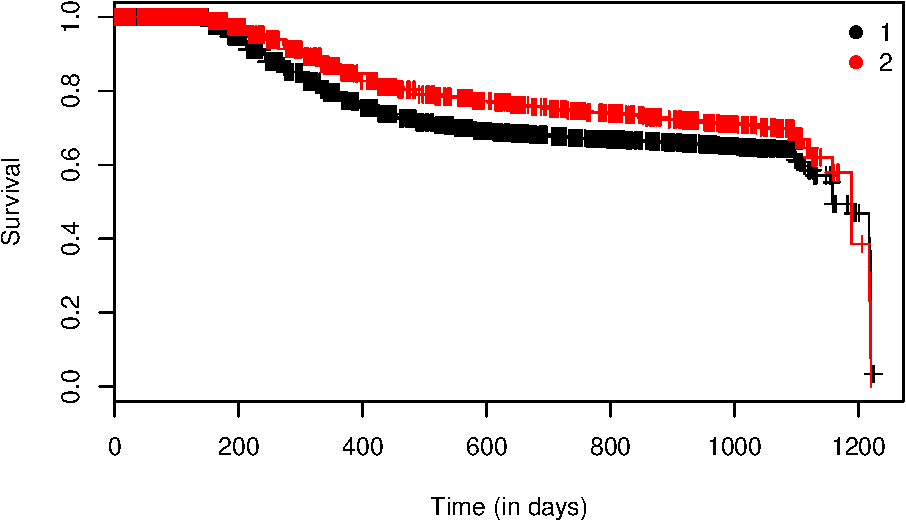
\includegraphics{bookdown_files/figure-latex/unnamed-chunk-18-1.pdf}

Now, the questions that arises is if \textbf{these two curves are
statistivally equivalent}. For answering it, we can use the
\textbf{log-rank test} \citep{mantel, CIS-11103}. This is the most
well-known and widely used method to test the null hypothesis of no
difference in survival between two or more independent groups. It is a
large-sample chi-square test that is obtained by constructing a two by
two contingency table at each distinct event time, and comparing the
failure rates between the two groups, conditional on the number at risk
in each group. The test compares the entire survival experience between
groups and can be thought of as a test of whether the survival curves
are identical or not.

\BeginKnitrBlock{rmdhint_sestelo}
When we state that two KM curves are \emph{statistically equivalent}, we
mean that, based on a testing procedure that compares the two curves in
some \emph{overall sense}, we do not have evidence to indicate that the
true (population) survival curves are different.
\EndKnitrBlock{rmdhint_sestelo}

The null hypothesis (\(H_0\)) of the testing procedure is that
\textbf{there is no overall difference between the two (or \(k\))
survival curves}. Under this \(H_0\), the log--rank statistic is
approximately a chi-square with \(k-1\) degree of freedom. Thus, tables
of the chi-square distribution are used to determine the pvalue.

This test is the one with most power to test differences that fit the
proportional hazards model - so works well as a set-up for subsequent
Cox regression. It gives equal weight to early and late failures.

An alternative test that is often used is the \textbf{Peto \& Peto}
\citep{CIS-11103} modification of the Gehan-Wilcoxon test
\citep{10.2307/2333825}. This last one is a variation of the log-rank
test statistic and is derived by applying different weights at the
\(f-\)th failure time. This approach is most sensitive to early
differences (or earlier time points) between survival.

This type of weighting may be used to assess whether the effect of a
treatment/marketing campaing on survival is strongest in the earlier
phases of administration/contacto and tends to be less effective over
time.

In the \textbf{absence of censoring}, these methods reduce to the
Wilcoxon-Mann-Whitney rank-sum test \citep{mann1947} for two samples and
to the Kruskal-Wallis test \citep{doi:10.1080/01621459.1952.10483441}
for more than two groups of survival times.

Of course, several other variations of the log-rank test statistic using
weights on each event time have been proposed in the literature
{[}\citet{CIS-23788}; \url{doi:10.1093/biomet/69.3.553};
10.2307/2289169{]}.

The log-rank test and the Peto \& Peto modification of the log-rank test
are both implemented in the \texttt{survdiff} function in library
\texttt{survival}.

\begin{Shaded}
\begin{Highlighting}[]
\KeywordTok{survdiff}\NormalTok{(}\KeywordTok{Surv}\NormalTok{(time, status) }\OperatorTok{~}\StringTok{ }\NormalTok{IsBorrowerHomeowner, }\DataTypeTok{data =}\NormalTok{ loan_filtered, }\DataTypeTok{rho =} \DecValTok{0}\NormalTok{) }\CommentTok{# log-rank}
\NormalTok{## Call:}
\NormalTok{## survdiff(formula = Surv(time, status) ~ IsBorrowerHomeowner, }
\NormalTok{##     data = loan_filtered, rho = 0)}
\NormalTok{## }
\NormalTok{##                              N Observed Expected (O-E)^2/E (O-E)^2/V}
\NormalTok{## IsBorrowerHomeowner=False 3342     1001      926      6.13      19.4}
\NormalTok{## IsBorrowerHomeowner=True  1581      362      437     12.98      19.4}
\NormalTok{## }
\NormalTok{##  Chisq= 19.4  on 1 degrees of freedom, p= 1.04e-05}

\KeywordTok{survdiff}\NormalTok{(}\KeywordTok{Surv}\NormalTok{(time, status) }\OperatorTok{~}\StringTok{ }\NormalTok{IsBorrowerHomeowner, }\DataTypeTok{data =}\NormalTok{ loan_filtered, }\DataTypeTok{rho =} \DecValTok{1}\NormalTok{)}\CommentTok{# peto & peto}
\NormalTok{## Call:}
\NormalTok{## survdiff(formula = Surv(time, status) ~ IsBorrowerHomeowner, }
\NormalTok{##     data = loan_filtered, rho = 1)}
\NormalTok{## }
\NormalTok{##                              N Observed Expected (O-E)^2/E (O-E)^2/V}
\NormalTok{## IsBorrowerHomeowner=False 3342      846      774      6.71      24.8}
\NormalTok{## IsBorrowerHomeowner=True  1581      294      366     14.18      24.8}
\NormalTok{## }
\NormalTok{##  Chisq= 24.8  on 1 degrees of freedom, p= 6.37e-07}

\CommentTok{# with more than 2 groups}
\KeywordTok{survdiff}\NormalTok{(}\KeywordTok{Surv}\NormalTok{(time, status) }\OperatorTok{~}\StringTok{ }\NormalTok{CreditGrade, }\DataTypeTok{data =}\NormalTok{ loan_filtered)}
\NormalTok{## Call:}
\NormalTok{## survdiff(formula = Surv(time, status) ~ CreditGrade, data = loan_filtered)}
\NormalTok{## }
\NormalTok{##                  N Observed Expected (O-E)^2/E (O-E)^2/V}
\NormalTok{## CreditGrade=A  428       42    115.5     46.77      51.8}
\NormalTok{## CreditGrade=AA 481       21    115.0     76.81      85.1}
\NormalTok{## CreditGrade=B  535       88    156.1     29.74      34.0}
\NormalTok{## CreditGrade=C  749      141    237.3     39.05      48.9}
\NormalTok{## CreditGrade=D  808      195    240.6      8.63      10.6}
\NormalTok{## CreditGrade=E  929      339    254.6     27.99      35.0}
\NormalTok{## CreditGrade=HR 915      487    223.8    309.49     378.5}
\NormalTok{## CreditGrade=NC  78       50     20.2     44.09      47.7}
\NormalTok{## }
\NormalTok{##  Chisq= 597  on 7 degrees of freedom, p= 0}
\end{Highlighting}
\end{Shaded}

If the null hyphotesis is rejected, we can apply a post-hoc analysis.
One approach would be to perform pairwise comparisons. This can be
achieved with the \texttt{pairwise\_survdiff} function of the package
\texttt{survminer} which calculates pairwise comparisons between group
levels with corrections for multiple testing.

\BeginKnitrBlock{rmdexercise_sestelo}
Use the function \texttt{pairwise\_survdiff} of the library
\texttt{survminer} in order to perform pairwise comparisons.
\EndKnitrBlock{rmdexercise_sestelo}

More beaitiful plots\ldots{}

\begin{Shaded}
\begin{Highlighting}[]
\KeywordTok{autoplot}\NormalTok{(model) }\CommentTok{#using ggplot2}
\end{Highlighting}
\end{Shaded}

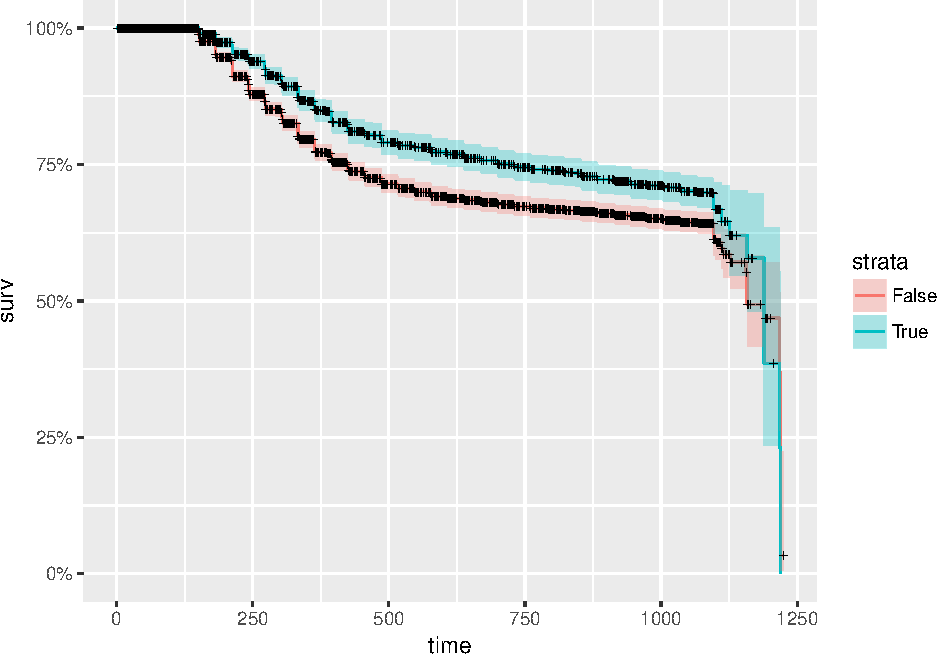
\includegraphics{bookdown_files/figure-latex/unnamed-chunk-22-1.pdf}

\begin{Shaded}
\begin{Highlighting}[]
\NormalTok{survminer}\OperatorTok{::}\KeywordTok{ggsurvplot}\NormalTok{(model)}
\end{Highlighting}
\end{Shaded}

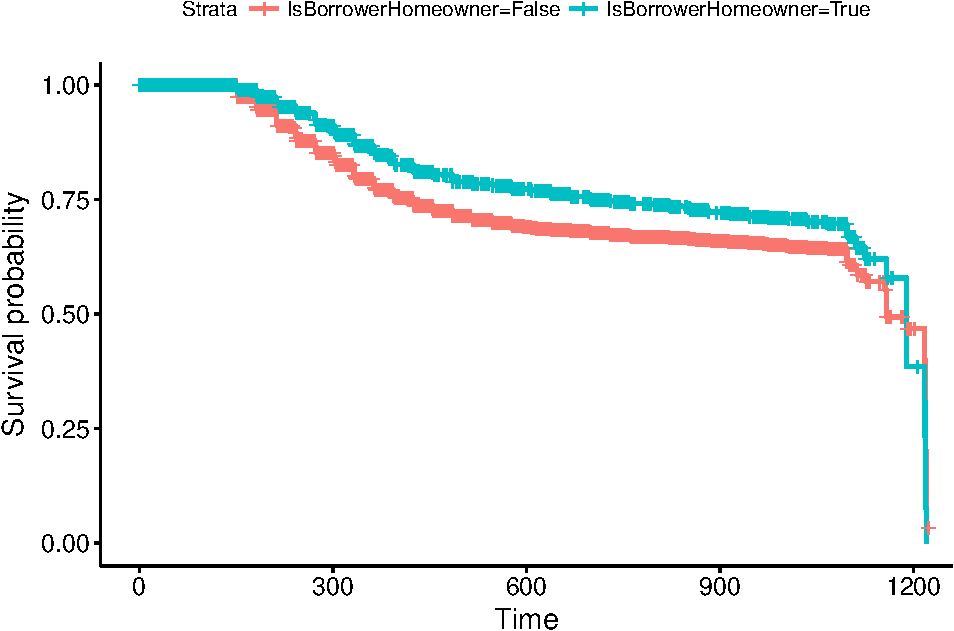
\includegraphics{bookdown_files/figure-latex/unnamed-chunk-22-2.pdf}

\begin{Shaded}
\begin{Highlighting}[]
\NormalTok{survminer}\OperatorTok{::}\KeywordTok{ggsurvplot}\NormalTok{(model, }\DataTypeTok{conf.int =} \OtherTok{TRUE}\NormalTok{)}
\end{Highlighting}
\end{Shaded}

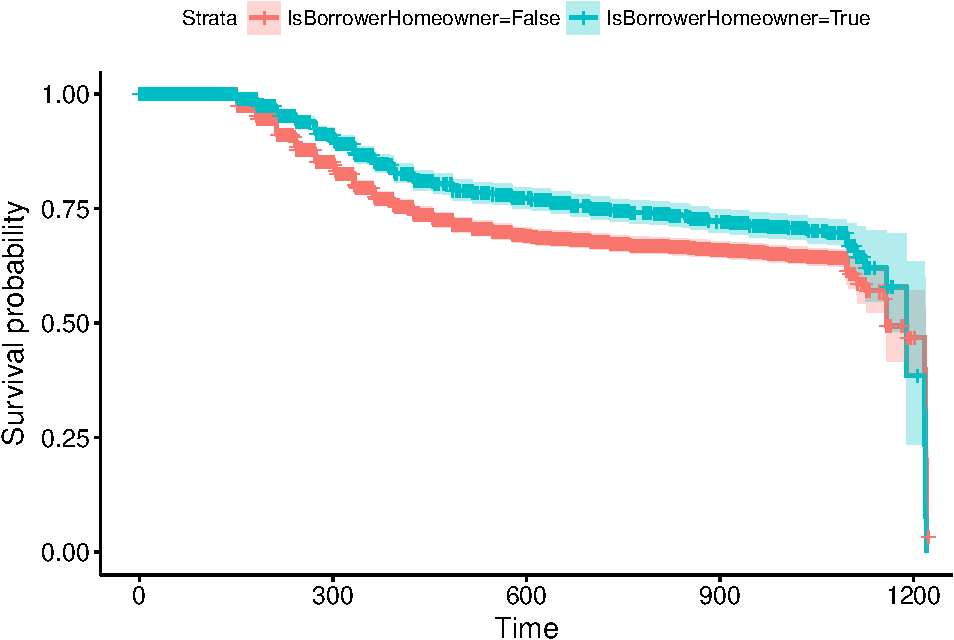
\includegraphics{bookdown_files/figure-latex/unnamed-chunk-22-3.pdf}

\section{Pros and Cons of the Kaplan-Meirs
estimator}\label{pros-and-cons-of-the-kaplan-meirs-estimator}

Pros:

\begin{itemize}
\tightlist
\item
  It is commonly used to describe survivor.
\item
  It is commonly used to compare two study populations.
\item
  It is intuitive graphical presentation.
\end{itemize}

Cons:

\begin{itemize}
\tightlist
\item
  It is mainly descriptive.
\item
  It does not control for covariates.
\item
  It can not accommodate time-dependent variables.
\end{itemize}

\BeginKnitrBlock{rmdexercise_sestelo}
With your dataset, obtain the estimated survival curve with the
Kaplan-Meier estimator for the time-to-event ``bring the payroll to the
BBVA''. Try to find some differences between type of client.
\EndKnitrBlock{rmdexercise_sestelo}

\chapter{The Cox Proportional Hazards Model}\label{cox}

This Chapter describes the Cox Proportional Hazards model, a very
popular statistical model used for analyzing survival data.

As we seen before, the survival function is the probability that the
time-to-event will be greater than some specified time and this
probability depends on:

\begin{itemize}
\item
  the \textbf{underlying hazard function} (how the risk of occurs the
  event per unit time changes over time at baseline covariates)
\item
  the \textbf{effect parameters} (how the hazard varies in response to
  the covariates)
\end{itemize}

We are going to use the Cox proportional hazards model to determine the
effect of the covariates on survival.

\section{The semiparametric model}\label{the-semiparametric-model}

A parametric survival model is one in which survival time (the outcome)
is assumed to follow a known distribution. Examples of distributions
that are commonly used for survival time are: the \textbf{Weibull}, the
\textbf{exponential} (a special case of the Weibull), the
\textbf{log-logistic}, the \textbf{log-normal}, etc.

The Cox proportional hazards model, by contrast, is not a fully
parametric model. Rather it is a \textbf{semi-parametric model} because
even if the regression parameters (the betas) are known, the
distribution of the outcome remains unknown. The baseline survival (or
hazard) function is not specified in a Cox model (we do not assume any
shape or form).

As before, let \(T\) denote the time to some event. Our data, based on a
sample of size \(n\), consists of the triple
\((\widetilde{T}_i, \Delta_i, \textbf{X}_i\), \(i = 1,...,n\) where
\(\widetilde{T}_i\) is the time on study for the \(i\)-th patient,
\(\Delta_i\) is the event indicator for the \(i\)-th patient
(\(\Delta_i=1\) if the event has occurred and \(\Delta_i=0\) if the
lifetime is right-censored) and
\(\textbf{X}_i= (X_{i1},\ldots, X_{ip})^t\) is the vector of covariates
or risk factors for the \(i\)-th individual which may affect the
survival distribution of \(T\).

\BeginKnitrBlock{rmdhint_sestelo}
Note that the covariates \(X_{ij}\), with \(j = 1, \ldots, p\), may be
time-dependent as \(\textbf X_i(t)=(X_{i1},\ldots,X_{ip})^t\) whose
value changes over time. This situation must be analyzed using the
\textbf{Extended Cox PH model}. However, for ease of presentation, we
shall consider the fixed-covariate case.
\EndKnitrBlock{rmdhint_sestelo}

The Cox PH regression model \citep{CIS-11133} is usually written in
terms of the hazard model formula as follows

\[
h(t, \textbf X) = h_0(t)  e^{\sum_{j=1}^p \beta_j X_j}.
\]

This model gives an expression for the hazard at time \(t\) for an
individual with a given specification of a set of explanatory variables
denoted by the bold \(\textbf X\).

Based on this model we can say that the hazard at time \(t\) is the
product of two quantities:

\begin{itemize}
\item
  The first of these, \(h_0(t)\), is called the \textbf{baseline hazard
  function} or the hazard for a reference individual with covariate
  values 0.
\item
  The second quantity is a \textbf{parametric component} which is a
  linear function of a set of \(p\) explanatory \(X\) variables that is
  exponentiated (it will be the \emph{relative risk} associated with
  covariate values \(X\)).
\end{itemize}

Note that an important feature of this model, which concerns the
\textbf{proportional hazards (PH) assumption}, is that the baseline
hazard is a function of \(t\), but does not involve the covariates. By
contrast, the exponential expresion involves the \(X\)'s but not the
time. The covariates here have a multiplicative effect and are called
\textbf{time-independent}.\footnote{It is possible, nevertheless, to
  consider covariates which do involve time. Such covariates are called
  \textbf{time-dependent} variables. When we consider these
  time-dependent covariates, the model is called the \textbf{extended
  Cox model} and in this case it no longer satisfies the proportional
  hazards assumption.}

Note that \textbf{the model is assuming proportional hazards} (the
hazard for any individual \(i\) is a fixed proportion of the hazard for
any other individual \(j\)), that is:

\[
\frac{h_i(t|\textbf X_i)}{h_j(t|\textbf X_j)} = exp(\boldsymbol \beta(\textbf X_i - \textbf X_j))
\]

or

\[
h_i(t|\textbf X_i) = \exp( \boldsymbol \beta(\textbf X_i - \textbf X_j)) h_j(t|\textbf X_j)
\] so hazard functions for each individual should be strictly parallel
and the hazard ratio is constant over time.

\section{Estimation}\label{estimation}

The estimation of the model is obtained by \textbf{Maximun Likelihood},
particularly maximazing the \textbf{``partial'' likelihood function}
rather than a (complete) likelihood function. The term ``partial''
likelihood is used because the likelihood formula considers
probabilities only for those subjects who fail, and does not explicitly
consider probabilities for those subjects who are censored. The
``partial'' likekihood is given by:

\[
L(\boldsymbol \beta) = \prod_{i:\Delta_i = 1} \frac{\exp\bigg[ \sum_{j=1}^{p}\beta_j X_{(i)j} \bigg]}{\sum_{k \in R(t_i)} \exp \bigg[ \sum_{j=1}^{p}\beta_j X_{(k)j} \bigg]}
\] being \(t_1 < t_2 < \ldots < t_D\) the ordered event times,
\(Z_{(i)j}\) the \(j\)-th covariate associated with the individual whose
failure time is \(t_i\) and \(R(t_i)\) the risk set at time \(t_i\),
that is, the the set of all individuals who are still under study at a
time just prior to \(t_i\).

Note that the numerator of the likelihood depends only on information
from the individual who experiences the event, whereas the denominator
uses information about all individuals who have not yet experienced the
event (including some individuals who will be censored later).

The \textbf{(partial) maximum likelihood} estimates are found by
maximizing the \(ln (L(\boldsymbol \beta))\) particularly, by taking
partial derivatives of \(ln (L(\boldsymbol \beta))\) with respect to
each parameter in the model, and then solving a system of equations. For
this algorithm such as Newton--Raphson \citep{doi:10.1137/1037125} or
Expectation-Maximitazion \citep{10.2307/2984875} are used.\footnote{In
  the presence of ties, the \citet{10.2307/1402659} or
  \citet{doi:10.1080/01621459.1977.10480613} approximations to the
  log-likelihood can be used.}

In \texttt{R}, we can estimate this model using the \texttt{coxph}
function of the \texttt{survival} package.

\begin{Shaded}
\begin{Highlighting}[]
\NormalTok{loan_filtered}\OperatorTok{$}\NormalTok{LoanOriginalAmount2 <-}\StringTok{  }\NormalTok{loan_filtered}\OperatorTok{$}\NormalTok{LoanOriginalAmount}\OperatorTok{/}\DecValTok{10000}

\NormalTok{model <-}\StringTok{ }\KeywordTok{coxph}\NormalTok{(}\KeywordTok{Surv}\NormalTok{(time, status) }\OperatorTok{~}\StringTok{ }\NormalTok{LoanOriginalAmount2 }\OperatorTok{+}\StringTok{ }\NormalTok{IsBorrowerHomeowner }\OperatorTok{+}
\StringTok{                 }\NormalTok{IncomeVerifiable, }\DataTypeTok{data =}\NormalTok{ loan_filtered) }
\end{Highlighting}
\end{Shaded}

For taking the \textbf{ties} into account we can use the \texttt{method}
argument

\begin{Shaded}
\begin{Highlighting}[]
\KeywordTok{coxph}\NormalTok{(}\KeywordTok{Surv}\NormalTok{(time, status) }\OperatorTok{~}\StringTok{ }\NormalTok{LoanOriginalAmount2 }\OperatorTok{+}\StringTok{ }\NormalTok{IsBorrowerHomeowner }\OperatorTok{+}
\StringTok{        }\NormalTok{IncomeVerifiable, }\DataTypeTok{data =}\NormalTok{ loan_filtered, }\DataTypeTok{method =} \StringTok{"efron"}\NormalTok{) }

\KeywordTok{coxph}\NormalTok{(}\KeywordTok{Surv}\NormalTok{(time, status) }\OperatorTok{~}\StringTok{ }\NormalTok{LoanOriginalAmount2 }\OperatorTok{+}\StringTok{ }\NormalTok{IsBorrowerHomeowner }\OperatorTok{+}
\StringTok{        }\NormalTok{IncomeVerifiable, }\DataTypeTok{data =}\NormalTok{ loan_filtered, }\DataTypeTok{method =} \StringTok{"breslow"}\NormalTok{) }

\KeywordTok{coxph}\NormalTok{(}\KeywordTok{Surv}\NormalTok{(time, status) }\OperatorTok{~}\StringTok{ }\NormalTok{LoanOriginalAmount2 }\OperatorTok{+}\StringTok{ }\NormalTok{IsBorrowerHomeowner }\OperatorTok{+}
\StringTok{        }\NormalTok{IncomeVerifiable, }\DataTypeTok{data =}\NormalTok{ loan_filtered, }\DataTypeTok{method =} \StringTok{"exact"}\NormalTok{) }
\end{Highlighting}
\end{Shaded}

\section{Computing the Hazard Ratio}\label{computing-the-hazard-ratio}

One of the main goals of the Cox PH model is to \textbf{compare the
hazard rates} of individuals who have different values for the
covariates. The idea is that we care more about comparing groups than
about estimating absolute survival. To this end, we are going to use the
\textbf{Hazard Ratio} (HR).

A hazard ratio is defined as the hazard for one individual divided by
the hazard for a different individual. The two individuals being
compared can be distinguished by their values for the set of predictors,
that is, the \(X\)'s. We can write the hazard ratio as the estimate of

\[
\widehat{HR} = \frac{\hat h_i(t|\textbf X_i)}{h_j(t|\textbf X_j)} = \frac{\hat h_0(t) \exp (\boldsymbol{\hat \beta} \textbf X_i)}{\hat h_0(t) \exp (\boldsymbol{\hat \beta}\textbf X_j)}=exp(\boldsymbol{\hat \beta}(\textbf X_i - \textbf X_j)).
\]

Additionally, we can construct a \((1-\alpha)\)\% confidence interval
for the hazard ratio as \[
\exp( \boldsymbol{\hat \beta}(\textbf X_i - \textbf X_j) \pm z_{1-\alpha/2} \hspace{0.2cm} \widehat{se}(\boldsymbol{\hat \beta}(\textbf X_i - \textbf X_j)), 
\] where
\(\widehat{se}(\boldsymbol{\hat \beta}(\textbf X_i - \textbf X_j))\) is
equal to
\(\sqrt{ \widehat{Var}(\boldsymbol{\hat \beta}(\textbf X_i - \textbf X_j))}\).

In order to understand what this hazard ratio means, we are going to see
same examples.

In the first one we are using \textbf{a discrete predictor}
(\texttt{smoking}) and we will see the hazard ratio for smoking versus
not smoking adjusted by the age. So, let
\(\textbf X_i:(smoking=1, age = 60)\) and
\(\textbf X_j:(smoking=0, age = 60)\), the hazard ratio is

\[
HR= \frac{h_i(t|\textbf X_i)}{h_j(t|\textbf X_j)} = \frac{h_0(t) e^{\beta_{smoking} \cdot 1 + \beta_{age} \cdot 60}}{h_0(t) e^{\beta_{age} \cdot 60}} = e^ {\beta_{smoking}}
\]

For example, if \(\beta_{smoking}= 0.5\), the hazard ratio for smoking
adjusted for age will be \(exp(0.5)= 1.65\). That is, the hazard of
death increases 65\% for smokers.

In the second example we use a \textbf{continuous predictor},
\texttt{age} of the individuals. Let
\(\textbf X_i:(smoking=0, age = 70)\) and
\(\textbf X_j:(smoking=0, age = 60)\), the hazard ratio for a ten years
increase in age adjusted by smoking is

\[
HR= \frac{h_i(t|\textbf X_i)}{h_j(t|\textbf X_j)} = \frac{h_0(t) e^{\beta_{smoking} \cdot 0 + \beta_{age} \cdot 70}}{h_0(t) e^{\beta_{smoking} \cdot 0+ \beta_{age} \cdot 60}} = e^{\beta_{age}(70-60)} = e^{\beta_{age}\cdot 10 = (e^{\beta_{age}})^{10} }
\]

Note that \(e^{\beta_{age}}\) is the hazard ratio for a 1-unit increase
in the predictor.

\BeginKnitrBlock{rmdhint_sestelo}
\textbf{Interpretation of the hazard ratio (like Odds Ratio in Logistic
Models)}

\begin{itemize}
\tightlist
\item
  HR = 1: no effect
\item
  HR \textgreater{} 1: increase in the hazard\\
\item
  HR \textless{} 1/10: reduction in the hazard

  \EndKnitrBlock{rmdhint_sestelo}
\end{itemize}

Moving again on the \texttt{R} code, we can see (by means of the
\texttt{summary} function) the hazard ratios for the covariates included
in the model

\begin{Shaded}
\begin{Highlighting}[]
\NormalTok{m1 <-}\StringTok{ }\KeywordTok{coxph}\NormalTok{(}\KeywordTok{Surv}\NormalTok{(time, status) }\OperatorTok{~}\StringTok{ }\NormalTok{LoanOriginalAmount2 }\OperatorTok{+}\StringTok{ }\NormalTok{IsBorrowerHomeowner }\OperatorTok{+}
\StringTok{              }\NormalTok{IncomeVerifiable, }\DataTypeTok{data =}\NormalTok{ loan_filtered) }
\KeywordTok{summary}\NormalTok{(m1)}
\NormalTok{## Call:}
\NormalTok{## coxph(formula = Surv(time, status) ~ LoanOriginalAmount2 + IsBorrowerHomeowner + }
\NormalTok{##     IncomeVerifiable, data = loan_filtered)}
\NormalTok{## }
\NormalTok{##   n= 4923, number of events= 1363 }
\NormalTok{## }
\NormalTok{##                             coef exp(coef) se(coef)      z Pr(>|z|)    }
\NormalTok{## LoanOriginalAmount2     -0.12177   0.88535  0.06661 -1.828   0.0675 .  }
\NormalTok{## IsBorrowerHomeownerTrue -0.24815   0.78025  0.06231 -3.982 6.82e-05 ***}
\NormalTok{## IncomeVerifiableTrue     0.29263   1.33995  0.30286  0.966   0.3339    }
\NormalTok{## ---}
\NormalTok{## Signif. codes:  0 '***' 0.001 '**' 0.01 '*' 0.05 '.' 0.1 ' ' 1}
\NormalTok{## }
\NormalTok{##                         exp(coef) exp(-coef) lower .95 upper .95}
\NormalTok{## LoanOriginalAmount2        0.8854     1.1295    0.7770    1.0088}
\NormalTok{## IsBorrowerHomeownerTrue    0.7802     1.2816    0.6905    0.8816}
\NormalTok{## IncomeVerifiableTrue       1.3399     0.7463    0.7401    2.4260}
\NormalTok{## }
\NormalTok{## Concordance= 0.558  (se = 0.008 )}
\NormalTok{## Rsquare= 0.005   (max possible= 0.988 )}
\NormalTok{## Likelihood ratio test= 24.46  on 3 df,   p=1.999e-05}
\NormalTok{## Wald test            = 23.33  on 3 df,   p=3.44e-05}
\NormalTok{## Score (logrank) test = 23.46  on 3 df,   p=3.238e-05}
\KeywordTok{termplot}\NormalTok{(m1, }\DataTypeTok{terms =} \StringTok{"IsBorrowerHomeowner"}\NormalTok{)}
\end{Highlighting}
\end{Shaded}

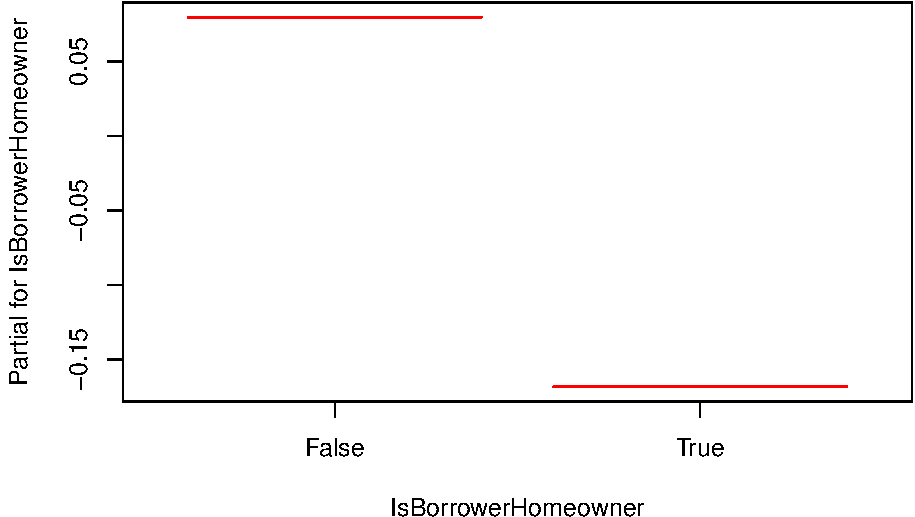
\includegraphics{bookdown_files/figure-latex/unnamed-chunk-28-1.pdf}

The estimated hazard ratio for \texttt{IsBorrowerHomeowner\ ==\ True} vs
\texttt{IsBorrowerHomeowner\ ==\ False} is 0.78 with a 95\% CI of (0.69,
0.88), that is, \texttt{IsBorrowerHomeowner\ ==\ True} has 0.78 times
the hazard of \texttt{IsBorrowerHomeowner\ ==\ False}, a 22\% lower
hazard rate. The estimated hazard ratio for
\texttt{IsBorrowerHomeowner\ ==\ False} vs
\texttt{IsBorrowerHomeowner\ ==\ True} is 1.28. Note that the procedure
is the same for the other covariates.

\section{Hypothesis testing}\label{hypothesis-testing}

In order to test the significance of a variable or a interaction term in
the model we can use two procedures:

\begin{itemize}
\item
  the \textbf{Wald test} (typically used with Maximun Likelihood
  estimates)
\item
  the \textbf{Likelihood Ratio test (LRT)} (it uses the log likelihood
  to compare two nested models)
\end{itemize}

The null hypothesis of the \textbf{Wald test} states that the coeficient
\(\beta_j\) is equal to 0. The test statistics is

\[
Z = \frac{\hat \beta_j - 0}{Std. Err (\hat \beta_j)} \sim N(0,1)
\]

\begin{Shaded}
\begin{Highlighting}[]
\KeywordTok{summary}\NormalTok{(m1)}\OperatorTok{$}\NormalTok{coef}
\NormalTok{##                               coef exp(coef)   se(coef)         z}
\NormalTok{## LoanOriginalAmount2     -0.1217675 0.8853542 0.06661063 -1.828049}
\NormalTok{## IsBorrowerHomeownerTrue -0.2481456 0.7802463 0.06231124 -3.982357}
\NormalTok{## IncomeVerifiableTrue     0.2926323 1.3399500 0.30286111  0.966226}
\NormalTok{##                             Pr(>|z|)}
\NormalTok{## LoanOriginalAmount2     6.754227e-02}
\NormalTok{## IsBorrowerHomeownerTrue 6.823526e-05}
\NormalTok{## IncomeVerifiableTrue    3.339311e-01}

\CommentTok{# by hand... for IncomeVerifiable}
\NormalTok{z <-}\StringTok{ }\KeywordTok{summary}\NormalTok{(m1)}\OperatorTok{$}\NormalTok{coef[}\DecValTok{3}\NormalTok{, }\DecValTok{1}\NormalTok{]}\OperatorTok{/}\KeywordTok{summary}\NormalTok{(m1)}\OperatorTok{$}\NormalTok{coef[}\DecValTok{3}\NormalTok{, }\DecValTok{3}\NormalTok{]  }
\NormalTok{pvalue <-}\StringTok{ }\DecValTok{2} \OperatorTok{*}\StringTok{ }\KeywordTok{pnorm}\NormalTok{(z, }\DataTypeTok{lower.tail =} \OtherTok{FALSE}\NormalTok{)}
\NormalTok{pvalue}
\NormalTok{## [1] 0.3339311}
\end{Highlighting}
\end{Shaded}

According to the pvalue of the test, the null hypothesis is accepted
(for the \texttt{IncomeVerifiable} variable). Thus, the model must not
include this variable.

The other approach is to use the \textbf{Likelihood Ratio test}. In this
case, we need to compute the difference between the log likelihood
statistic of the \emph{reduced model} which does not contain the
variable that we want to test and the log likelihood statistic of the
\emph{full model} containing the variable. In general, the LRT statistic
can be written in the form of

\[
LRT = -2 ln \frac{L_R}{L_F}= 2 ln(L_F) - 2 ln(L_R) \sim \chi^2_p
\] where \(L_R\) denotes the log likelihood of the reduced model with
\(k\) parameter and \(L_F\) is the log likelihood of the full model with
\(k + p\) parameters. \(\chi^2_p\) is a Chi-square with \(p\) degrees of
freedom, where \(p\) denotes the number of predictors being assessed.

\BeginKnitrBlock{rmdhint_sestelo}
In general, the Likelihood Ratio test and Wald statistics may not give
exactly the same answer. It has been shown that of the two test
procedures, the LR statistic has better statistical properties, so when
in doubt, you should use the \textbf{LRT}.
\EndKnitrBlock{rmdhint_sestelo}

\begin{Shaded}
\begin{Highlighting}[]

\NormalTok{m_red <-}\StringTok{ }\KeywordTok{coxph}\NormalTok{(}\KeywordTok{Surv}\NormalTok{(time, status) }\OperatorTok{~}\StringTok{ }\NormalTok{LoanOriginalAmount2 }\OperatorTok{+}\StringTok{ }\NormalTok{IsBorrowerHomeowner,}
               \DataTypeTok{data =}\NormalTok{ loan_filtered) }
\KeywordTok{anova}\NormalTok{(m_red, m1) }\CommentTok{#fist the reduced, second the full}
\NormalTok{## Analysis of Deviance Table}
\NormalTok{##  Cox model: response is  Surv(time, status)}
\NormalTok{##  Model 1: ~ LoanOriginalAmount2 + IsBorrowerHomeowner}
\NormalTok{##  Model 2: ~ LoanOriginalAmount2 + IsBorrowerHomeowner + IncomeVerifiable}
\NormalTok{##   loglik  Chisq Df P(>|Chi|)}
\NormalTok{## 1 -10837                    }
\NormalTok{## 2 -10836 1.0297  1    0.3102}

\CommentTok{# by hand... for IncomeVerifiable variable}
\NormalTok{m1}\OperatorTok{$}\NormalTok{loglik  }\CommentTok{# the first is the log likelihood of a model that contains}
\NormalTok{## [1] -10848.75 -10836.52}
           \CommentTok{#      none of the predictors, so we need the second one}

\NormalTok{chi <-}\StringTok{ }\DecValTok{2} \OperatorTok{*}\StringTok{ }\NormalTok{m1}\OperatorTok{$}\NormalTok{loglik[}\DecValTok{2}\NormalTok{] }\OperatorTok{-}\StringTok{ }\DecValTok{2} \OperatorTok{*}\StringTok{ }\NormalTok{m_red}\OperatorTok{$}\NormalTok{loglik[}\DecValTok{2}\NormalTok{]}
\NormalTok{pvalue <-}\StringTok{ }\DecValTok{1} \OperatorTok{-}\StringTok{ }\KeywordTok{pchisq}\NormalTok{(chi, }\DataTypeTok{df =} \DecValTok{1}\NormalTok{) }\CommentTok{# df = 3 - 2}
\NormalTok{pvalue}
\NormalTok{## [1] 0.310227}
\end{Highlighting}
\end{Shaded}

In this case, using an \(\alpha = 0.05\) and testing the significance of
the \texttt{IncomeVerifiable} variable, we must remove it from the
model.

\section{Adjusting Survival Curves}\label{adjusting-survival-curves}

From a survival analysis point of view, we want to obtain also estimates
for the survival curve. Remember that if we do not use a model, we can
apply the Kaplan-Meier estimator. However, when a Cox model is used to
fit survival data, survival curves can be obtained adjusted for the
explanatory variables used as predictors. These are called
\textbf{adjusted survival curves} and, like Kaplan-Meier curves, these
are also plotted as step functions.

The hazard formula seen before can be converted to a survival function
as

\[
S(t|\textbf X) = \bigg[ S_0(t) \bigg]^{e^{\sum_{j=1}^p \beta_j X_j}}.
\]

This survival function formula is the basis for determining adjusted
survival curves. The estimates of \(\hat S_0(t)\) and \(\hat b_j\) are
provided by the computer program that fits the Cox model. The \(X\)'s,
however, must first be specified by the investigator before the computer
program can compute the estimated survival curve.

\BeginKnitrBlock{rmdhint_sestelo}
Typically, when computing adjusted survival curves, the value chosen for
a covariate being adjusted is an average value like an arithmetic mean
or a median.
\EndKnitrBlock{rmdhint_sestelo}

The \texttt{survfit} function estimates \(S(t)\), by default at the mean
values of the covariates:

\begin{Shaded}
\begin{Highlighting}[]
\NormalTok{m2 <-}\StringTok{ }\NormalTok{m_red}
\NormalTok{newdf <-}\StringTok{ }\KeywordTok{data.frame}\NormalTok{(}\DataTypeTok{IsBorrowerHomeowner =} \KeywordTok{levels}\NormalTok{(loan_filtered}\OperatorTok{$}\NormalTok{IsBorrowerHomeowner), }
                    \DataTypeTok{LoanOriginalAmount2 =} \KeywordTok{rep}\NormalTok{(}\KeywordTok{mean}\NormalTok{(loan_filtered}\OperatorTok{$}\NormalTok{LoanOriginalAmount2), }\DecValTok{2}\NormalTok{))}
\NormalTok{fit <-}\StringTok{ }\KeywordTok{survfit}\NormalTok{(m2, }\DataTypeTok{newdata =}\NormalTok{ newdf)}
\CommentTok{#summary(fit) # to see the estimated values}
\KeywordTok{plot}\NormalTok{(fit, }\DataTypeTok{conf.int =} \OtherTok{TRUE}\NormalTok{, }\DataTypeTok{col =} \KeywordTok{c}\NormalTok{(}\DecValTok{1}\NormalTok{,}\DecValTok{2}\NormalTok{))}
\KeywordTok{legend}\NormalTok{(}\StringTok{"bottomleft"}\NormalTok{, }\KeywordTok{levels}\NormalTok{(newdf[,}\DecValTok{1}\NormalTok{]), }\DataTypeTok{col =} \KeywordTok{c}\NormalTok{(}\DecValTok{1}\NormalTok{, }\DecValTok{2}\NormalTok{), }\DataTypeTok{lty =} \KeywordTok{c}\NormalTok{(}\DecValTok{1}\NormalTok{,}\DecValTok{1}\NormalTok{))}
\end{Highlighting}
\end{Shaded}

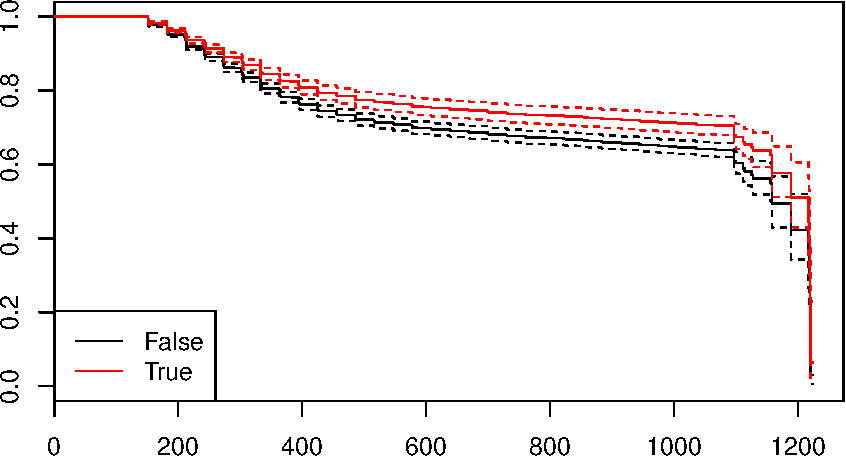
\includegraphics{bookdown_files/figure-latex/unnamed-chunk-33-1.pdf}

\begin{Shaded}
\begin{Highlighting}[]
\CommentTok{# another option using the survminer package}
\NormalTok{survminer}\OperatorTok{::}\KeywordTok{ggsurvplot}\NormalTok{(fit)}
\end{Highlighting}
\end{Shaded}

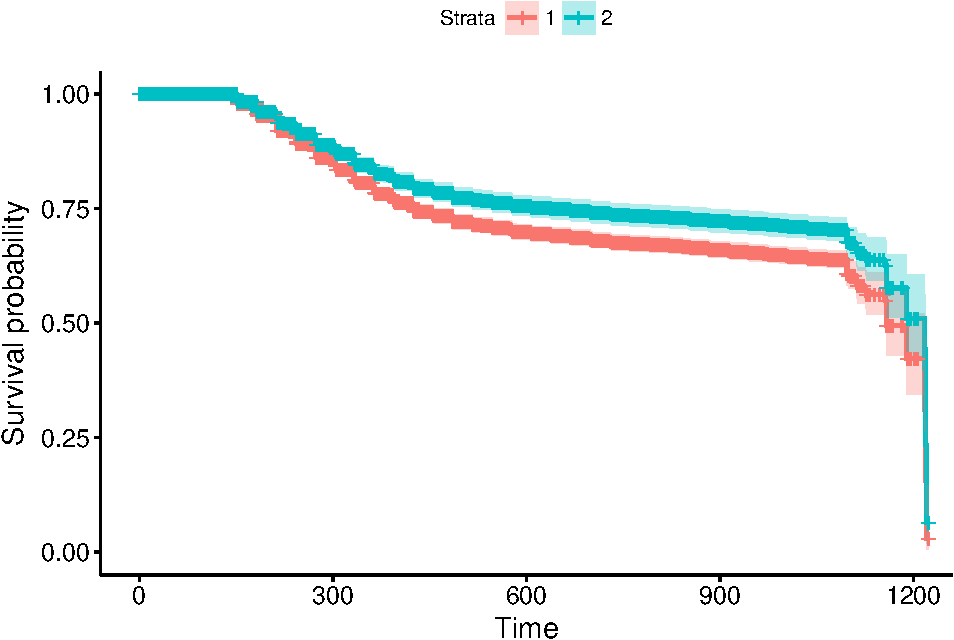
\includegraphics{bookdown_files/figure-latex/unnamed-chunk-34-1.pdf}

\begin{Shaded}
\begin{Highlighting}[]
\CommentTok{# easier... without refitting}
\KeywordTok{ggcoxadjustedcurves}\NormalTok{(m2, }\DataTypeTok{data =}\NormalTok{ loan_filtered, }
                    \DataTypeTok{variable =}\NormalTok{ loan_filtered}\OperatorTok{$}\NormalTok{IsBorrowerHomeowner)}
\end{Highlighting}
\end{Shaded}

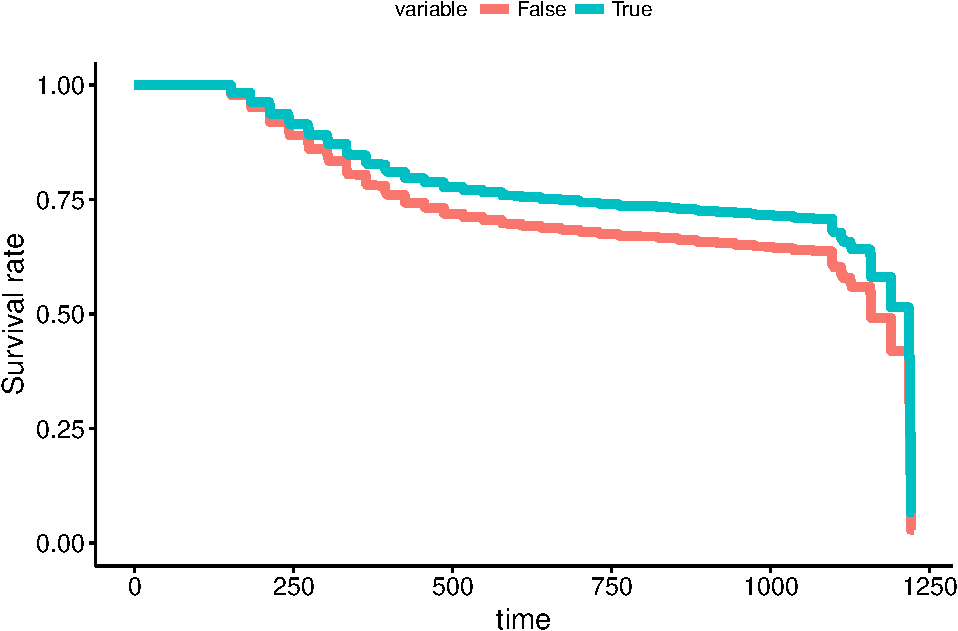
\includegraphics{bookdown_files/figure-latex/unnamed-chunk-35-1.pdf}

\BeginKnitrBlock{rmdhint_sestelo}
For some help with the \texttt{survminer} package\ldots{} Download the
cheatsheet
\href{http://www.sthda.com/english/rpkgs/survminer/survminer_cheatsheet.pdf}{here}.
\EndKnitrBlock{rmdhint_sestelo}

\BeginKnitrBlock{rmdexercise_sestelo}
Try to estimate a Cox PH model using your dataset.
\EndKnitrBlock{rmdexercise_sestelo}

\section{How to evaluate the PH
assumption?}\label{how-to-evaluate-the-ph-assumption}

Now we are going to illustrate two methods to evaluate the proportional
hazards assumptions: one \textbf{graphical approach} and one
\textbf{goodness-of-fit test}. Recall that the Hazard Ratio that
compares two specifications of the covariates (defined as
\(\textbf{X}^*\) and \(\textbf{X}\)) can be expressed as

\[
HR = \exp(\sum_{j=1}^p \beta_j (X_j^* - X_j)) 
\] where \(\textbf{X}^*=(X_1^*, X_2^*, \ldots, X_j^*)\) and
\(\textbf{X}=(X_1, X_2, \ldots, X_j)\), and proportionally of hazards
assumption indicates that this quantity is constant over time.
Equivalently, this means that the hazard for one individual is
proportional to the hazard for any other individual, where the
proportionality constant is independent of time.

\BeginKnitrBlock{rmdhint_sestelo}
\textbf{Think about this\ldots{}}

It is important to note that if the graph of the \textbf{hazards cross}
for two or more categories of a predictor of interest, the \textbf{PH
assumption is not met}. However, althought the hazard functions do not
cross, it is possible that the PH assumption is not met. Thus, rather
than checking for crossing hazards, we need to use other apporaches.
\EndKnitrBlock{rmdhint_sestelo}

\subsection{Graphical approach}\label{graphical-approach}

The most popular graphical techniques for evaluating the PH assumption
involves comparing estimated \textbf{--ln(--ln) survival curves} over
different (combinations of) categories of variables being investigated.

A log--log survival curve is simply a transformation of an estimated
survival curve that results from taking the natural log of an estimated
survival probability twice.\footnote{Note that the scale of the y-axis
  of an estimated survival curve ranges between 0 and 1, whereas the
  corresponding scale for a -ln(-ln) curve ranges between \(-\infty\)
  and \(+\infty\).}

As we said, the hazard function can be rewritten as \[
S(t|\textbf X) = \bigg[ S_0(t) \bigg]^{e^{\sum_{j=1}^p \beta_j X_j}}
\] and once we applied the -ln(-ln), the expression can be rewritten as
\[
-\ln \bigg[-\ln S(t|\textbf X) \bigg] =  - \sum_{j=1}^p \beta_j X_j - \ln  \bigg[-\ln S_0(t|\textbf X) \bigg].  
\]

Now, considering two different specifications of the covariates,
corresponding to two different individuals, \(\textbf X_1\) and
\(\textbf X_2\), and subtracting the second log--log curve from the
first yields the expression

\[
-\ln \bigg[-\ln S(t|\textbf X_1) \bigg] = -\ln \bigg[-\ln S(t|\textbf X_2) \bigg] + \sum_{j=1}^p \beta_j (X_{1j} - X_{2j}) 
\]

This expression indicates that if we use a Cox model (well-used) and
plot the estimated log-log survival curves for individuals on the same
graph, the two plots would be approximately parallel. The distance
between the two curves is the linear expression involving the
differences in predictor values, which does not involve time.

Note that there is an \textbf{important problem} associated with this
approach, that is, \textbf{how to decide} ``how parallel is parallel?''.
This fact can be subjective, thus the proposal is to be conservative for
this decision by assuming the PH assumption is satisfied unless there is
strong evidence of nonparallelism of the log--log curves.

Now we are going to check the proportinal hazards assumption for the
variable \texttt{IsBorrowerHomeowner}. This can be done by plotting
\textbf{log-log Kaplan Meier survival estimates} against time (or
against the log of time) and evaluating whether the curves are
reasonably parallel.

\begin{Shaded}
\begin{Highlighting}[]
\NormalTok{km_home <-}\StringTok{ }\KeywordTok{survfit}\NormalTok{(}\KeywordTok{Surv}\NormalTok{(time, status) }\OperatorTok{~}\StringTok{ }\NormalTok{IsBorrowerHomeowner, }\DataTypeTok{data =}\NormalTok{ loan_filtered)}
\CommentTok{#autoplot(km_home) # just to see the km curves}

\KeywordTok{plot}\NormalTok{(km_home, }\DataTypeTok{fun =} \StringTok{"cloglog"}\NormalTok{, }\DataTypeTok{xlab =} \StringTok{"Time (in days) using log"}\NormalTok{,}
     \DataTypeTok{ylab =} \StringTok{"log-log survival"}\NormalTok{, }\DataTypeTok{main =} \StringTok{"log-log curves by clinic"}\NormalTok{) }
\end{Highlighting}
\end{Shaded}

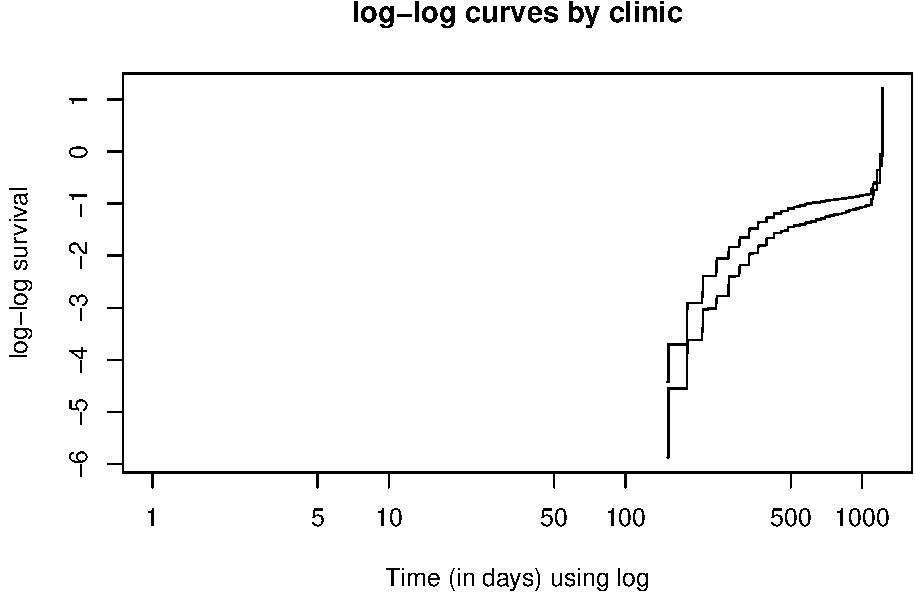
\includegraphics{bookdown_files/figure-latex/unnamed-chunk-39-1.pdf}

\begin{Shaded}
\begin{Highlighting}[]
\CommentTok{# another option}
\KeywordTok{ggsurvplot}\NormalTok{(km_home, }\DataTypeTok{fun =} \StringTok{"cloglog"}\NormalTok{)}
\end{Highlighting}
\end{Shaded}

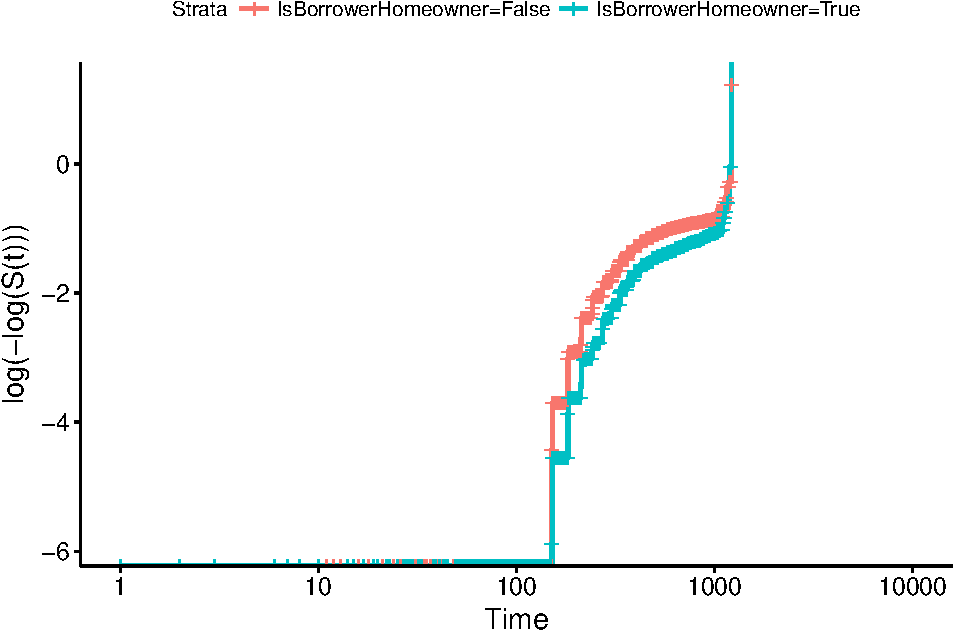
\includegraphics{bookdown_files/figure-latex/unnamed-chunk-40-1.pdf}

It seems that \textbf{the proportional hazards assumption is violated}
as the log-log survival curves are not parallel.

Another graphical option could be to use the \textbf{Schoenfeld
residuals} to examine model fit and detect outlying covariate values.
Shoenfeld residuals represent the difference between the observed
covariate and the expected given the risk set at that time. They should
be flat, centered about zero.

\begin{Shaded}
\begin{Highlighting}[]
\KeywordTok{ggcoxdiagnostics}\NormalTok{(m2, }\DataTypeTok{type =} \StringTok{"schoenfeld"}\NormalTok{)}
\end{Highlighting}
\end{Shaded}

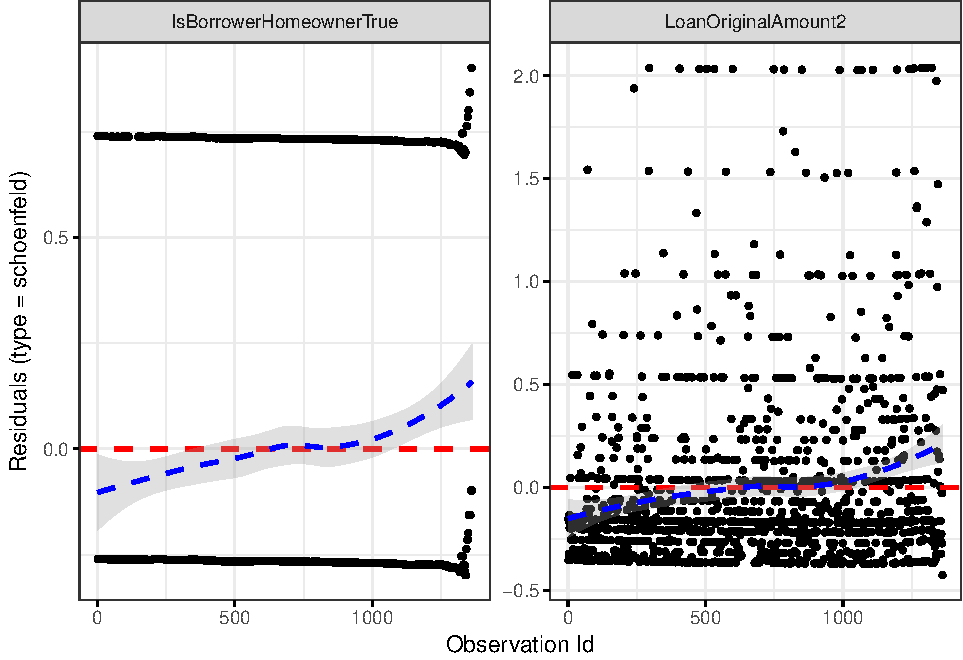
\includegraphics{bookdown_files/figure-latex/unnamed-chunk-41-1.pdf}

\begin{Shaded}
\begin{Highlighting}[]
\CommentTok{# another option}
\NormalTok{zph <-}\StringTok{ }\KeywordTok{cox.zph}\NormalTok{(m2)}
\KeywordTok{par}\NormalTok{(}\DataTypeTok{mfrow =} \KeywordTok{c}\NormalTok{(}\DecValTok{1}\NormalTok{, }\DecValTok{2}\NormalTok{))}
\KeywordTok{plot}\NormalTok{(zph, }\DataTypeTok{var =} \DecValTok{1}\NormalTok{)}
\KeywordTok{plot}\NormalTok{(zph, }\DataTypeTok{var =} \DecValTok{2}\NormalTok{)}
\end{Highlighting}
\end{Shaded}

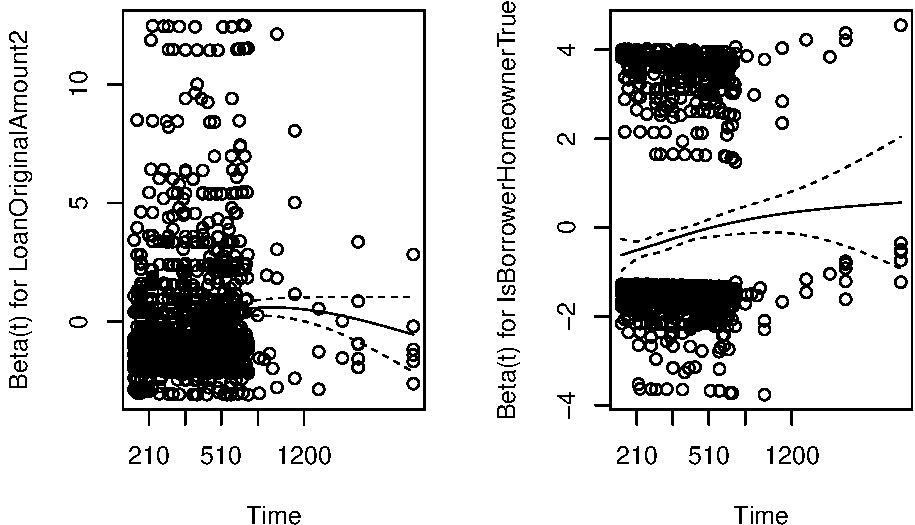
\includegraphics{bookdown_files/figure-latex/unnamed-chunk-42-1.pdf}

\subsection{Goodness-of-fit test}\label{goodness-of-fit-test}

A second approach for assessing the PH assumption involves
\textbf{goodness-of-fit (GOF) tests}. To this end, different test have
been proposed in the literature
\citep{1568a5d7e9974c31be97c0ff34c233a7}. We focuss in the
\citet{Harrell86}, a variation of a test originally proposed by
\citet{doi:10.1093/biomet/69.1.239}. This is a test of
\textbf{correlation between the Schoenfeld residuals and survival time}.
A correlation of zero indicates that the model met the proportional
hazards assumption (the null hypothesis).

This can be applied by means of the \texttt{cox.zph} function of the
\texttt{survival} package.

\begin{Shaded}
\begin{Highlighting}[]
\KeywordTok{cox.zph}\NormalTok{(m2)}
\NormalTok{##                           rho chisq        p}
\NormalTok{## LoanOriginalAmount2     0.130  27.1 1.96e-07}
\NormalTok{## IsBorrowerHomeownerTrue 0.103  14.0 1.81e-04}
\NormalTok{## GLOBAL                     NA  49.3 1.96e-11}
\end{Highlighting}
\end{Shaded}

It seems again that the proportional hazards assumption is not satisfied
(as we saw with the log-log survival curves).

\section{Non-Proportional Hazards\ldots{} and now
what?}\label{non-proportional-hazards-and-now-what}

A insignificant nonproportionality may make no difference to the
interpretation of a dataset, particularly for large sample sizes. What
if the nonproportionality is large and real? Possible approaches are
possible in the context of the Cox model itself:

\begin{itemize}
\item
  \textbf{Stratify}. Covariates with nonproportional effects may be
  incorporated into the model as stratification factors rather than
  predictors (but\ldots{} be careful, stratification works naturally for
  categorical variables, however for quantitative variables you would
  have to discretize).
\item
  \textbf{Partition of the time axis}, if the proportional hazards
  assumption holds for short time periods but not for the entire study.
\item
  \textbf{Nonlinear effect}. Continuous covariates with nonlinear effect
  may lead to nonproportional effects.
\end{itemize}

\subsection{An example\ldots{} Stratified Proportional Hazards
Models}\label{an-example-stratified-proportional-hazards-models}

Sometimes the proportional hazard assumption is violated for some
covariate. In such cases, it is possible to stratify taking this
variable into account and use the proportional hazards model in each
stratum for the other covariates. We include in the model predictors
that satify the proportional hazard assumption and remove from it the
predictor that is stratified.

Now, the subjects in the \(z\)-th stratum have an arbitrary baseline
hazard function \(h_{0z}(t)\) and the effect of other explanatory
variables on the hazard function can be represented by a proportional
hazards model in that stratum.

In the Stratified Proportional Hazards Model the regression coefficients
are assumed to be the same for each stratum although the baseline hazard
functions may be different and completely unrelated.

\begin{Shaded}
\begin{Highlighting}[]
\NormalTok{m3 <-}\StringTok{ }\KeywordTok{coxph}\NormalTok{(}\KeywordTok{Surv}\NormalTok{(time, status) }\OperatorTok{~}\StringTok{ }\NormalTok{LoanOriginalAmount2  }\OperatorTok{+}
\StringTok{              }\KeywordTok{strata}\NormalTok{(IsBorrowerHomeowner), }\DataTypeTok{data =}\NormalTok{ loan_filtered) }
\KeywordTok{summary}\NormalTok{(m3)}
\NormalTok{## Call:}
\NormalTok{## coxph(formula = Surv(time, status) ~ LoanOriginalAmount2 + strata(IsBorrowerHomeowner), }
\NormalTok{##     data = loan_filtered)}
\NormalTok{## }
\NormalTok{##   n= 4923, number of events= 1363 }
\NormalTok{## }
\NormalTok{##                         coef exp(coef) se(coef)      z Pr(>|z|)  }
\NormalTok{## LoanOriginalAmount2 -0.11967   0.88721  0.06667 -1.795   0.0726 .}
\NormalTok{## ---}
\NormalTok{## Signif. codes:  0 '***' 0.001 '**' 0.01 '*' 0.05 '.' 0.1 ' ' 1}
\NormalTok{## }
\NormalTok{##                     exp(coef) exp(-coef) lower .95 upper .95}
\NormalTok{## LoanOriginalAmount2    0.8872      1.127    0.7785     1.011}
\NormalTok{## }
\NormalTok{## Concordance= 0.54  (se = 0.01 )}
\NormalTok{## Rsquare= 0.001   (max possible= 0.983 )}
\NormalTok{## Likelihood ratio test= 3.35  on 1 df,   p=0.06731}
\NormalTok{## Wald test            = 3.22  on 1 df,   p=0.07264}
\NormalTok{## Score (logrank) test = 3.22  on 1 df,   p=0.07255}
\end{Highlighting}
\end{Shaded}

You can see that the output is similar to previous model without
stratification however, in this case, we do not have information about
the hazard ratio of the stratification variable,
\texttt{IsBorrowerHomeowner}. This variable is not really in the model.
In any case, you can plot it\ldots{}

\begin{Shaded}
\begin{Highlighting}[]
\KeywordTok{ggsurvplot}\NormalTok{(}\KeywordTok{survfit}\NormalTok{(m3), }\DataTypeTok{data =}\NormalTok{ loan_filtered, }\DataTypeTok{conf.int =} \OtherTok{TRUE}\NormalTok{)}
\end{Highlighting}
\end{Shaded}

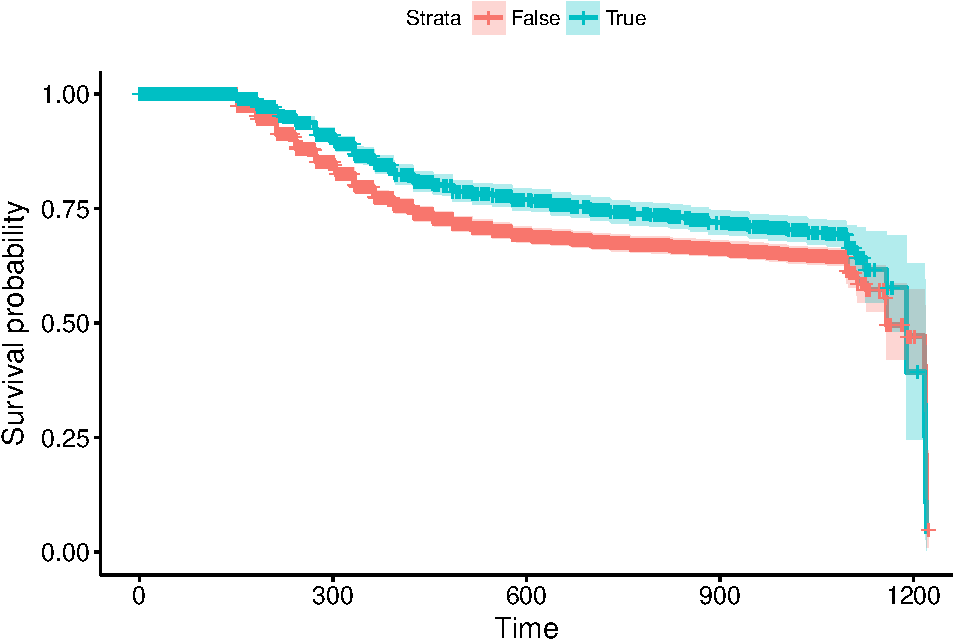
\includegraphics{bookdown_files/figure-latex/unnamed-chunk-45-1.pdf}

\BeginKnitrBlock{rmdexercise_sestelo}
Check the proportional hazard assumption of the Cox PH model estimated
in your dataset.
\EndKnitrBlock{rmdexercise_sestelo}

\section{Why Cox PH model is so popular? (pros of the
model)}\label{why-cox-ph-model-is-so-popular-pros-of-the-model}

\begin{itemize}
\item
  It is a ``robust'' model, so that the results from using the Cox model
  will closely approximate the results for the correct parametric model
  (even though the baseline hazard is not specified).
\item
  The specific form of the model - which gives the hazard function as a
  product of a baseline hazard involving \(t\) and an exponential
  expression involving the \(X\)'s without \(t\) - is very interesting.
  The exponential part of this product is appealing because it ensures
  that the fitted model will always give estimated hazards that are
  non-negative (this is perfect, because by definition, the value of the
  hazard function must range between zero and plus infinity).
\item
  Although the baseline hazard part of the model is unspecified, we can
  estimate the betas in the exponential part of the model (as we have
  seen). Then, the hazard function \(h(t,\textbf X)\) and its
  corresponding survival curves \(S(t, \textbf X\)) can also be
  estimated.
\item
  Finally, it is preferred over the logistic model when survival time
  information is available and there is censoring. Because you can
  obtain more information!
\end{itemize}

\section{Bonus track 1: Additive Cox
model}\label{bonus-track-1-additive-cox-model}

The Cox PH model assumes a linear effect of the predictors. If the true
effect is highly nonlinear this can lead to a nonproportinal hazards or
misleading statistical conclusions.

One alternative approach is to use an Additive Cox model
\citep{NoRefworks:5} of the form

\[
h(t, \textbf X) = h_0(t) e^{\sum_{j=1}^p f_j(\textbf X_j)}
\] with \(f_j\) being an unknown and smooth function.

In order to estimate this model one could use the
\href{https://cran.r-project.org/web/packages/mgcv/index.html}{\texttt{mgcv}}
package as follows

\begin{Shaded}
\begin{Highlighting}[]
\NormalTok{m4 <-}\StringTok{ }\NormalTok{mgcv}\OperatorTok{::}\KeywordTok{gam}\NormalTok{(time }\OperatorTok{~}\StringTok{ }\KeywordTok{s}\NormalTok{(LoanOriginalAmount2) }\OperatorTok{+}\StringTok{ }\NormalTok{IsBorrowerHomeowner, }
                \DataTypeTok{data =}\NormalTok{ loan_filtered, }\DataTypeTok{family =} \StringTok{"cox.ph"}\NormalTok{, }\DataTypeTok{weights =}\NormalTok{ status)}
\KeywordTok{summary}\NormalTok{(m4)}
\NormalTok{## }
\NormalTok{## Family: Cox PH }
\NormalTok{## Link function: identity }
\NormalTok{## }
\NormalTok{## Formula:}
\NormalTok{## time ~ s(LoanOriginalAmount2) + IsBorrowerHomeowner}
\NormalTok{## }
\NormalTok{## Parametric coefficients:}
\NormalTok{##                         Estimate Std. Error z value Pr(>|z|)    }
\NormalTok{## IsBorrowerHomeownerTrue -0.23344    0.06248  -3.736 0.000187 ***}
\NormalTok{## ---}
\NormalTok{## Signif. codes:  0 '***' 0.001 '**' 0.01 '*' 0.05 '.' 0.1 ' ' 1}
\NormalTok{## }
\NormalTok{## Approximate significance of smooth terms:}
\NormalTok{##                          edf Ref.df Chi.sq  p-value    }
\NormalTok{## s(LoanOriginalAmount2) 4.853  5.857  26.91 0.000206 ***}
\NormalTok{## ---}
\NormalTok{## Signif. codes:  0 '***' 0.001 '**' 0.01 '*' 0.05 '.' 0.1 ' ' 1}
\NormalTok{## }
\NormalTok{## Deviance explained = 0.818%}
\NormalTok{## -REML =  10848  Scale est. = 1         n = 4923}
\KeywordTok{plot}\NormalTok{(m4, }\DataTypeTok{pages =} \DecValTok{1}\NormalTok{, }\DataTypeTok{all.terms =} \OtherTok{TRUE}\NormalTok{)}
\end{Highlighting}
\end{Shaded}

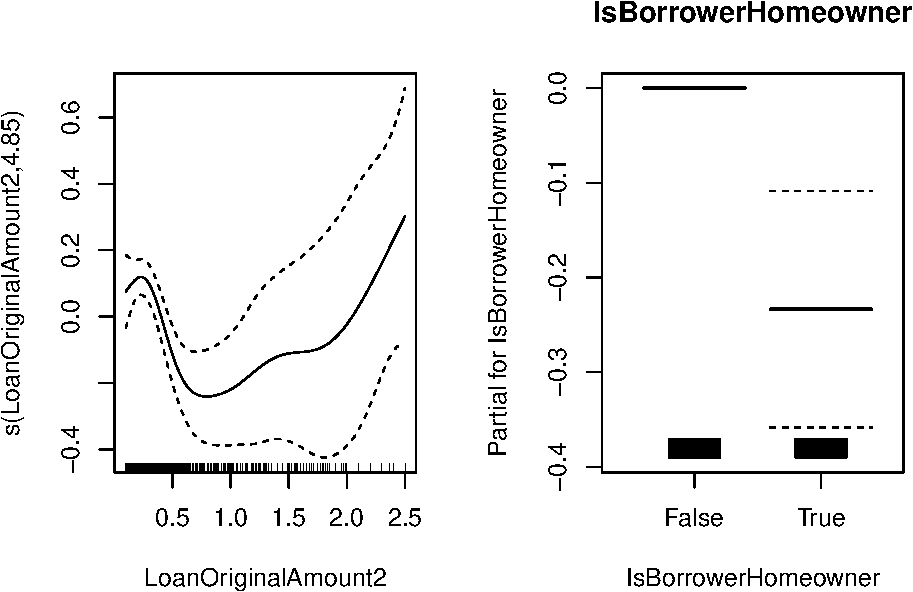
\includegraphics{bookdown_files/figure-latex/unnamed-chunk-47-1.pdf}

\BeginKnitrBlock{rmdhint_sestelo}
Note the change in the sintaxis compared with the previous examples. The
status indicator in used in the \texttt{weights} argument.
\EndKnitrBlock{rmdhint_sestelo}

\section{Bonus track 2: Machine Learning for estimating the Cox PM
model}\label{bonus-track-2-machine-learning-for-estimating-the-cox-pm-model}

The
\href{https://cran.r-project.org/web/packages/rpart/index.html}{\texttt{rpart}}
package builds R's basic tree models of survival data. For an overview
you can consult the section 8.4 of the rpart
\href{https://cran.r-project.org/web/packages/rpart/vignettes/longintro.pdf}{vignette}.

Additionally, the new package
\href{https://cran.r-project.org/web/packages/ranger/index.html}{\texttt{ranger}}
\citep{Wright:2017aa} is a fast implementation of the Random Forests
algorithm for building ensembles of classification and regression trees,
working also with survival data. Since \texttt{ranger()} uses standard
`Surv survival objects, it's an ideal tool for getting acquainted with
survival analysis in this machine-learning age.

Under construction!

\chapter{Joint Models for Longitudinal and Time-to-Event
Data}\label{joint-models-for-longitudinal-and-time-to-event-data}

In this Chapter we will see a joint modelling approach in order to
analyze \textbf{two types of outcomes} produced usually in longitudinal
studies, particularly, a set of \textbf{longitudinal response
measurements} and the \textbf{time to an event of interest}, such as
default, death, etc.

These two outcomes are usually analyzed separately, using a
\textbf{mixed effects model} ((CITAS)) for the longitudinal response and
a \textbf{survival model} for the time-to-event. Here, we are going to
see how we can analyze them jointly.

\subsubsection*{Why should I use these type of
models?}\label{why-should-i-use-these-type-of-models}
\addcontentsline{toc}{subsubsection}{Why should I use these type of
models?}

As we mentioned in Chapter \ref{cox}, the Cox PH hazard model can be
extended in order to incorporate time-dependent variables. However, when
we focus our interest in the time-to-event and we wish to take into
account the effect of the longitudinal variable as a time-dependent
covariate, \textbf{traditional approaches} for analyzing time-to-event
data (such as the partial likelihood for the Cox proportional hazards
models) \textbf{are not applicable in all situations}. In particular,
\textbf{standard time-to-event models require that time-dependent
covariates are external}; that is, the value of this covariate at time
point \(t\) is not affected by the occurrence of an event at time point
\(u\), with \(t > u\) \citep[Section 6.3]{kalbfleisch1980statistical}.
However, the type of time-dependent covariates that we have in
longitudinal studies do not met this condition, this is due to the fact
that they are the output of a stochastic process generated by the
subject, which is directly related to the failure mechanism. Based on
this, in order to produce correct inferences, we need to apply a joint
model that takes into account the joint distribution of the longitudinal
and survival outcomes.

\textbf{Another advantage} of these models is that they allow to deal
with the \textbf{error measurements} in the time dependent variables
(longitudinal variable in this case). In a Cox model with time dependent
covariates we assume that the variables are measured without error.

\BeginKnitrBlock{rmdhint_sestelo}
When we think in time-dependent covariates, we should first distinguish
between two different categories, namely, \textbf{internal or
endogenous} covariates or \textbf{external or exogenous} covariates.
Internal covariates are generated from the patient herself and therefore
require the existence of the patient, for example \emph{CD4 cell count}
and the hazard for death by HIV are stochastic processes generated by
the patient herself. On the other hand, \emph{air pollution} is an
external covariate to asthma attacks, since the patient has no influence
on air pollution.
\EndKnitrBlock{rmdhint_sestelo}

\section{Linear Mixed Models}\label{linear-mixed-models}

As we mentioned, \textbf{Joint Models} take two outcomes into account,
the \textbf{longitudinal response} and the \textbf{survival time}. In
order to estimate these type of models, we need first to fit a model for
the longitudinal response (usually a \textbf{linear mixed model}) and
then for the survival time. I am assuming here that you have understood
entirely the Chapter \ref{cox} and you do not have any problem with the
estimation of the Cox model by means of the \texttt{coxph} function.
Regarding the linear mixed model you can see an brief introduction with
examples below using the
\href{https://cran.r-project.org/web/packages/nlme/index.html}{\texttt{nlme}}
package. For a good overview you can consult the Chapter 2 of
\citet{book:1606416}.

So, our focus in this part is on longitudinal data. This data can be
defined as the data resulting from the \textbf{observations of subjects}
(e.g., human beings, animals, etc.) that are \textbf{measured repeatedly
over time}. From this descriptions, it is evident that in a longitudinal
setting we expect repeated measurements taken on the same subject to
exhibit positive correlation. This feature implies that standard
statistical tools, such as the t-test and simple linear regression that
assume independent observations, are not appropriate for longitudinal
data analysis (they may produce invalid standard errors). In order to
solve this situation and obtain valid inference, one possible approach
is to use a \textbf{mixed model}, a regression method for continuous
outcomes that models longitudinal data by assuming, for example,
\textbf{random errors within a subject} and \textbf{random variation in
the trajectory among subjects}.

We are going to explain briefly this approach. Figure \ref{fig:mixed}
shows an example with hypothetical longitudinal data for two subjects.
In this figure, monthly observations are recorded for up to one year.
Note that each subject appears to have their own linear trajectory but
with small fluctuations about the line. This fluctuations are referred
to as the \textbf{within-subject variation} in the outcomes. Note that
if we only have data from one person these will be the typical error
term in regression. The dashed line in the center of the figure shows
the average of individual linear-time trajectories. This line
characterizes the \textbf{average for the population} as a function of
time. For example, the value of the dashed line at month 2 is the mean
response if the observation (at two months) for all subjects was
averaged. Thus, this line represents both the typical trajectory and the
population average as a function of time.

The main idea of \textbf{Linear Mixed Model} is that they make specific
assumptions about the variation in observations attributable to
\textbf{variation within a subject} and to \textbf{variation among
subjects}. To formally introduce this representation of longitudinal
data, we let \(Y_{ij}\) denote the response of subject
\(i, i = 1, \ldots, n\) at time \(X_{ij}, j = 1,...,n_i\) and
\(\beta_{i0} + \beta_{i1} X_{ij}\) denote the line that characterizes
the observation path for \(i\). Note that each subject has an
individual-specific intercept and slope. Note that

\begin{itemize}
\item
  The \textbf{within-subject variation} is seen as the deviation between
  individual observations, \(Y_{ij}\), and the individual linear
  trajectory, that is \(Y_{ij} - (\beta_{i0} + \beta_{i1} X_{ij})\).
\item
  The \textbf{between-subject variation} is represented by the variation
  among the intercepts, \(var(\beta_{i0})\) and the variation among
  subject in the slopes \(var(\beta_{i1})\).
\end{itemize}

\begin{figure}

{\centering 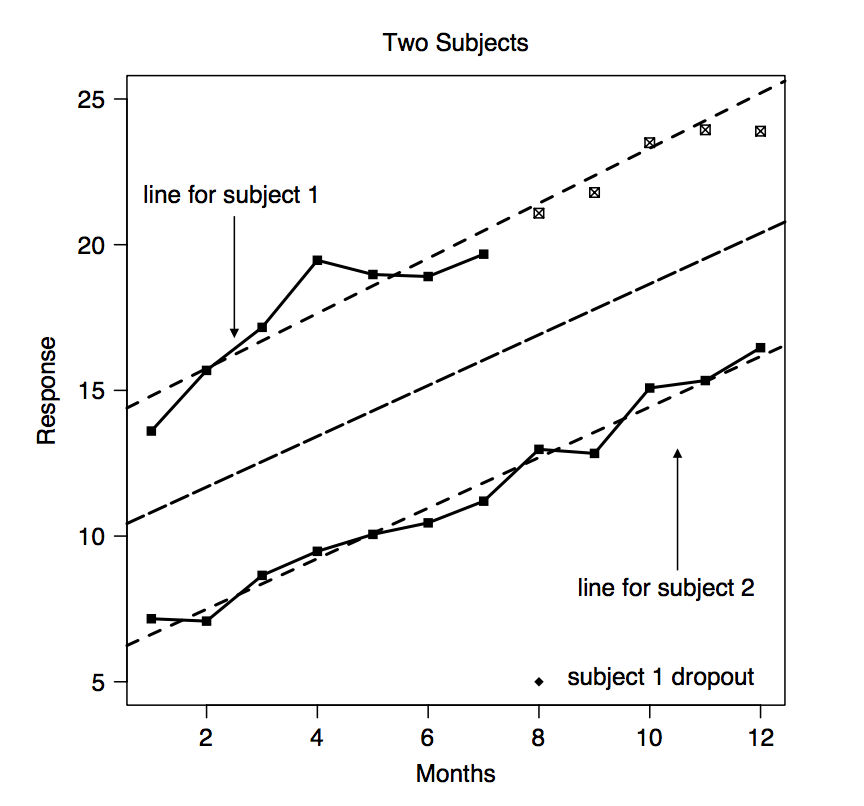
\includegraphics[width=12in]{images//mixed_image} 

}

\caption{Hypothetical longitudinal data for two subjects.}\label{fig:mixed}
\end{figure}

Figure \ref{fig:mixed} taken from \citet{bio}.

If parametric assumptions are made regarding the within- and
between-subject components of variation, it is possibel to use
\emph{maximum likelihood methods} for estimating the regression
parameters (which characterize the population average), and the variance
components (which characterize the magnitude of within- and
between-subject heterogeneity). For continuous outcomes it is a good
idea to assume that within-subject errors are normally distributed and
to assume that intercepts and slopes are normally distributed among
subjects. This will be

\begin{itemize}
\tightlist
\item
  within-subjects: \[
  E(Y_{ij}|\beta_i) = \beta_{i,0} + \beta_{i, 1} X_{ij}
  \]
\end{itemize}

\[
Y_{ij} = \beta_{i,0} + \beta_{i, 1} X_{ij} + \varepsilon_{ij}
\]

\[
 \varepsilon_{ij} \sim N(0, \sigma^2)
\]

\begin{itemize}
\tightlist
\item
  between-subjects:
\end{itemize}

{[} \bigg(

\begin{array}{c} \beta_{i,0}\\ \beta_{i,1}\\ \end{array}

\bigg) \sim

N
\bigg[ \bigg(\begin{array}{c} \beta_{0}\\ \beta_{1}\\ \end{array} \bigg),  \bigg(\begin{array}{c} D_{00} & D_{01}\\ D_{10} & D_{11}\\ \end{array} \bigg)   \bigg]
{]} where \(D\) is the variance-covariance matrix of the random effects,
with \(D_00= var(b_{i,0})\) and \(D_11= var(b_{i,1})\).

If we think in \(b_{i,0}= (\beta_{i,0} - \beta_0)\) and
\(b_{i,1}= (\beta_{i,1} - \beta_1)\), the model can be written as

\[
Y_{ij} = \beta_0 + \beta_1 X_{ij} + b_{i,0} + b_{i,1} X_{ij} + \varepsilon_{ij}
\] where \$ b\_\{i,0\}\$ and \(b_{i,1}\) represent deviations from the
population average intercept and slope respectively. In this equation
there is \emph{systematic} variation (given by the two first betas) and
a \textbf{random} variation (the rest).

The random component is partitioned into the observation level and
subject level fluctuations: that is, the between-subject
(\(b_{i,0} + b_{i,1} X_{ij}\)) and within-subject (\(\varepsilon_{ij}\))
variations.

A more general form including \(p\) predictors is

\[
Y_{ij} = \beta_0 + \beta_1 X_{ij,1} +\ldots +  + \beta_p X_{ij,p} + b_{i,0} + b_{i,1} X_{ij,1} + \ldots + b_{i,p} X_{ij,p}+ \varepsilon_{ij}
\]

\[
Y_{ij} = X_{ij}'\beta + Z_{ij}' b_i + \varepsilon_{ij}
\] where \(X_{ij}'=[X_{ij,1}, X_{ij,2}, \ldots, X_{ij,p}]\) and
\(Z_{ij}'=[X_{ij,1}, X_{ij,2}, \ldots, X_{ij,q}]\). In general way, we
assume that the covariates in \(Z_{ij}\) are a subset of the variables
in \(X_{ij}\) and thus \(q < p\).

\BeginKnitrBlock{rmdhint_sestelo}
It is important to highlighted that based on this model the coefficient
of covariate \(k\) for subject \(i\) is given as \((\beta_k + b_{i,k})\)
if \(k \le q\), and is simply \(\beta_k\) if \(q < k \le p\).
Therefore,inalinearmixed model there may be some regression parameters
that vary among subjects while some regression parameters are common to
all subjects.
\EndKnitrBlock{rmdhint_sestelo}

Moving again onto the example, it seems that each subject has their own
intercept, but the subjects may have a common slope. So, a
\textbf{random intercept} model assumes parallel trajectories for any
two subjects and is given as a special case of the general mixed model:

\[
Y_{ij} = \beta_0 + \beta_1 X_{ij,1} + b_{i,0} + \varepsilon_{ij}.
\]

Using the above model, the intercept for subject \(i\) is given by
\(\beta_0 + b_{i,0}\) while the slope for subject \(i\) is simply
\(\beta_1\) since there is no additional random slope, \(b_{i,1}\) in
the random intercept model.

If we assume that the slope for each individual \(i\) can also be
different, we have to use a \textbf{random intercept and slope} model of
the type

\[
Y_{ij} = \beta_0 + \beta_1 X_{ij,1} + b_{i,0} + b_{i,1} X_{ij,1}+ \varepsilon_{ij}.
\] and now the intercept for subject \(i\) is given by
\(\beta_0 + b_{i,0}\) while the slope for subject \(i\) is
\(\beta_1 + b_{i, 1}\).

In order to fit these models, we can use the \texttt{lme} function of
the \texttt{nlme} package.

\begin{Shaded}
\begin{Highlighting}[]
\KeywordTok{head}\NormalTok{(aids) }
\NormalTok{##   patient  Time death       CD4 obstime drug gender prevOI         AZT}
\NormalTok{## 1       1 16.97     0 10.677078       0  ddC   male   AIDS intolerance}
\NormalTok{## 2       1 16.97     0  8.426150       6  ddC   male   AIDS intolerance}
\NormalTok{## 3       1 16.97     0  9.433981      12  ddC   male   AIDS intolerance}
\NormalTok{## 4       2 19.00     0  6.324555       0  ddI   male noAIDS intolerance}
\NormalTok{## 5       2 19.00     0  8.124038       6  ddI   male noAIDS intolerance}
\NormalTok{## 6       2 19.00     0  4.582576      12  ddI   male noAIDS intolerance}
\NormalTok{##   start  stop event}
\NormalTok{## 1     0  6.00     0}
\NormalTok{## 2     6 12.00     0}
\NormalTok{## 3    12 16.97     0}
\NormalTok{## 4     0  6.00     0}
\NormalTok{## 5     6 12.00     0}
\NormalTok{## 6    12 18.00     0}
\CommentTok{# CD4: square root CD4 cell count measurements}
\CommentTok{# obstime: time points at which the corresponding longitudinal response was recorded}
\end{Highlighting}
\end{Shaded}

\begin{Shaded}
\begin{Highlighting}[]
\CommentTok{# random-intercepts model (single random effect term for each patient)}

\NormalTok{fit1 <-}\StringTok{ }\KeywordTok{lme}\NormalTok{(}\DataTypeTok{fixed =}\NormalTok{ CD4 }\OperatorTok{~}\StringTok{ }\NormalTok{obstime, }\DataTypeTok{random =} \OperatorTok{~}\StringTok{ }\DecValTok{1} \OperatorTok{|}\StringTok{ }\NormalTok{patient, }\DataTypeTok{data =}\NormalTok{ aids)}
\KeywordTok{summary}\NormalTok{(fit1)}
\NormalTok{## Linear mixed-effects model fit by REML}
\NormalTok{##  Data: aids }
\NormalTok{##        AIC      BIC    logLik}
\NormalTok{##   7176.633 7197.618 -3584.316}
\NormalTok{## }
\NormalTok{## Random effects:}
\NormalTok{##  Formula: ~1 | patient}
\NormalTok{##         (Intercept) Residual}
\NormalTok{## StdDev:    4.506494 1.961662}
\NormalTok{## }
\NormalTok{## Fixed effects: CD4 ~ obstime }
\NormalTok{##                 Value  Std.Error  DF   t-value p-value}
\NormalTok{## (Intercept)  7.188663 0.22061320 937  32.58492       0}
\NormalTok{## obstime     -0.148500 0.01218699 937 -12.18513       0}
\NormalTok{##  Correlation: }
\NormalTok{##         (Intr)}
\NormalTok{## obstime -0.194}
\NormalTok{## }
\NormalTok{## Standardized Within-Group Residuals:}
\NormalTok{##         Min          Q1         Med          Q3         Max }
\NormalTok{## -3.84004681 -0.44310988 -0.05388055  0.43593364  6.09265321 }
\NormalTok{## }
\NormalTok{## Number of Observations: 1405}
\NormalTok{## Number of Groups: 467}
\end{Highlighting}
\end{Shaded}

Note that the estimation for the variability or the variance components,
that is, the variance of the errors (\(\varepsilon_{ij}\), within
personal errors) and the variance between subject (the variance of the
\(b_{i, 0}\)) are given under \emph{Random effects} heading. Under
\texttt{(Intercept)} we can see the estimated standard desviation for
the \(b_{i,0}\) coefficients and under \texttt{Residual}, the estimated
desviation for \(\varepsilon_{ij}\).

\begin{Shaded}
\begin{Highlighting}[]
\CommentTok{# variance of the beta_i0}
\KeywordTok{getVarCov}\NormalTok{(fit1)}
\NormalTok{## Random effects variance covariance matrix}
\NormalTok{##             (Intercept)}
\NormalTok{## (Intercept)      20.308}
\NormalTok{##   Standard Deviations: 4.5065}

\CommentTok{# standard desviation of e_ij}
\NormalTok{fit1}\OperatorTok{$}\NormalTok{sigma}
\NormalTok{## [1] 1.961662}

\CommentTok{# total variance of the model}
\KeywordTok{getVarCov}\NormalTok{(fit1)[}\DecValTok{1}\NormalTok{] }\OperatorTok{+}\StringTok{ }\NormalTok{fit1}\OperatorTok{$}\NormalTok{sigma}\OperatorTok{**}\DecValTok{2} 
\NormalTok{## [1] 24.15661}

\CommentTok{# % variance within person}
\NormalTok{(fit1}\OperatorTok{$}\NormalTok{sigma}\OperatorTok{**}\DecValTok{2}\OperatorTok{/}\NormalTok{(}\KeywordTok{getVarCov}\NormalTok{(fit1)[}\DecValTok{1}\NormalTok{] }\OperatorTok{+}\StringTok{ }\NormalTok{fit1}\OperatorTok{$}\NormalTok{sigma}\OperatorTok{**}\DecValTok{2}\NormalTok{)) }\OperatorTok{*}\StringTok{ }\DecValTok{100} 
\NormalTok{## [1] 15.92988}

\CommentTok{# % variance between person}
\NormalTok{(}\KeywordTok{getVarCov}\NormalTok{(fit1)[}\DecValTok{1}\NormalTok{]}\OperatorTok{/}\NormalTok{(}\KeywordTok{getVarCov}\NormalTok{(fit1)[}\DecValTok{1}\NormalTok{] }\OperatorTok{+}\StringTok{ }\NormalTok{fit1}\OperatorTok{$}\NormalTok{sigma}\OperatorTok{**}\DecValTok{2}\NormalTok{)) }\OperatorTok{*}\StringTok{ }\DecValTok{100} 
\NormalTok{## [1] 84.07012}
\end{Highlighting}
\end{Shaded}

The total variation in CD4 is estimated as 24.16. So, the proportion of
total variation that is attributed to within-person variability is
15.93\% with 84.07\% of total variation attributable to individual
variation in their general level of CD4 (attributable to random
intercepts).

The estimated regression coefficients \(\beta\) are provided under the
\emph{Fixed effects} heading. As expected, the coefficient for the time
effect has a negative sign indicating that on average the square root
CD4 cell counts declines in time.

Well, this random-intercepts model poses the unrealistic restriction
that the correlation between the repeated measurements remains constant
over time (we are not includiying the random slope yet). So, a natural
extension is a more flexible specification of the covariance structure
with the random-intercepts and random-slopes model. This model
introduces an additional random effects term, and assumes that the rate
of change in the CD4 cell count is different from patient to patient.

\begin{Shaded}
\begin{Highlighting}[]
\CommentTok{# random-intercepts and random-slopes model}
\NormalTok{fit2 <-}\StringTok{ }\KeywordTok{lme}\NormalTok{(CD4 }\OperatorTok{~}\StringTok{ }\NormalTok{obstime, }\DataTypeTok{random =} \OperatorTok{~}\StringTok{ }\NormalTok{obstime }\OperatorTok{|}\StringTok{ }\NormalTok{patient, }\DataTypeTok{data =}\NormalTok{ aids) }\CommentTok{# the intercept is  included by default}
\KeywordTok{summary}\NormalTok{(fit2)}
\NormalTok{## Linear mixed-effects model fit by REML}
\NormalTok{##  Data: aids }
\NormalTok{##        AIC     BIC    logLik}
\NormalTok{##   7141.282 7172.76 -3564.641}
\NormalTok{## }
\NormalTok{## Random effects:}
\NormalTok{##  Formula: ~obstime | patient}
\NormalTok{##  Structure: General positive-definite, Log-Cholesky parametrization}
\NormalTok{##             StdDev    Corr  }
\NormalTok{## (Intercept) 4.5898645 (Intr)}
\NormalTok{## obstime     0.1728724 -0.152}
\NormalTok{## Residual    1.7507904       }
\NormalTok{## }
\NormalTok{## Fixed effects: CD4 ~ obstime }
\NormalTok{##                 Value  Std.Error  DF  t-value p-value}
\NormalTok{## (Intercept)  7.189048 0.22215494 937 32.36051       0}
\NormalTok{## obstime     -0.150059 0.01518146 937 -9.88435       0}
\NormalTok{##  Correlation: }
\NormalTok{##         (Intr)}
\NormalTok{## obstime -0.218}
\NormalTok{## }
\NormalTok{## Standardized Within-Group Residuals:}
\NormalTok{##         Min          Q1         Med          Q3         Max }
\NormalTok{## -4.31679141 -0.41425035 -0.05227632  0.41094183  4.37413201 }
\NormalTok{## }
\NormalTok{## Number of Observations: 1405}
\NormalTok{## Number of Groups: 467}
\end{Highlighting}
\end{Shaded}

We observe very minor differences in the estimated fixed-effect
parameters compared with the previous model.

For the random effects, we can observe that there is greater variability
between patients in the baseline levels of CD4 (given by
\texttt{(Intercept)} variance) than in the evolutions of the marker in
time (\texttt{obstime} variance).

\section{Estimation of the Joint
Model}\label{estimation-of-the-joint-model}

In this section we are going to present the joint modelling framework
motivated by the \textbf{time-to-event point of view}, that is, we want
to add a time-dependent covariate measured with error in a survival
model.

Let \(T_i\) denote the observed failure time for the \(i\)-th subject
\((i = 1,...,n)\), which is taken as the minimum of the true event time
\(T_i\) and the censoring time \(C_i\), i.e.,
\(\widetilde T_i = \min(T_i,C_i)\). Furthermore, we define the event
indicator as \(\Delta_i = I(T_i \le C_i)\), where \(I\) is the indicator
function that takes the value 1 if the condition \(T_i \le C_i\) is
satisfied, and 0 otherwise. So, the observed data for the time-to-event
outcome consist of the pairs
\(\{(\widetilde T_i, \Delta_i), i = 1, . . . , n\}\). For the
longitudinal responses, let \(y_i(t)\) denote the value of the
longitudinal outcome at time point \(t\) for the \(i\)-th subject. Note
that we do not actually observe \(y_i(t)\) at all time points, but only
at the very specific occasions \(t_{ij}\) at which measurements were
taken. Thus, the observed longitudinal data consist of the measurements
\(y_{ij} = \{yi(t_{ij}),j = 1,...,n_i\}\).

The objective is to associate the \textbf{true} and \textbf{unobserved}
value of the longitudinal outcome at time \(t\), denoted by \(m_i(t)\),
with the event outcome \(\widetilde T_i\). Note that \(m_i(t)\) is
different from \(y_i(t)\) because this last is contaminated with
measurement error value of the longitudinal outcome at time \(t\).

In order to quantify the effect of \(m_i(t)\) on the risk of an event,
we can use a relative risk model of the form:

\begin{equation}
h_i(t|\mathcal{M}_i(t),w_i) = h_0(t) \exp \{ \gamma^t w_i + \alpha m_i(t) \}
\label{eq:joint}
\end{equation}

where \(\mathcal{M}_i(t)=\{ m_i(s), 0 \le s < t\}\) denotes the denotes
the history of the true unobserved longitudinal process up to time point
\(t\), \(h_0(\cdot)\) denotes the baseline risk function, and \(w_i\) is
a vector of baseline covariates (such as a treatment indicator, history
of diseases, etc.) with a corresponding vector of regression
coefficients \(\gamma\). Similarly, parameter \(\alpha\) quantifies the
effect of the underlying longitudinal outcome to the risk for an event.

\BeginKnitrBlock{rmdhint_sestelo}
The interpretation of \(\gamma\) and \(\alpha\) is exactly the same as
we have seen in Chapter \ref{cox}. In particular, \(exp(\gamma_j)\)
denotes the ratio of hazards for one unit change in \(w_{ij}\) at any
time \(t\), whereas \(exp(\alpha)\) denotes the relative increase in the
risk for an event at time \(t\) that results from one unit increase in
\(m_i(t)\) at the same time point.
\EndKnitrBlock{rmdhint_sestelo}

To complete the specification of teh above model, we need to think about
the choice for the baseline risk function \(h_0(\cdot)\). In standard
survival analysis it is customary to leave \(h_0(\cdot)\) completely
unspecified in order to avoid the impact of misspecifying the
distribution of survival times. However, within the joint modeling
framework, it turns out that following such a route may lead to an
underestimation of the standard errors of the parameter estimates
\citep{BIOM:BIOM570}. To avoid such problems we will need to explicitly
define \(h_0(\cdot)\), for example with a known parametric distribution
or alternatively, and even more preferably, we can opt for a parametric
but flexible specification of the baseline risk function. Several
approaches are implemented in the \texttt{JM} package under the argument
\texttt{method}.

\subsubsection*{The longitudinal
submodel}\label{the-longitudinal-submodel}
\addcontentsline{toc}{subsubsection}{The longitudinal submodel}

In the model above we use \(m_i(t)\) to denote the true value of the
underlying longitudinal covariate at time point \(t\). However, and as
mentioned earlier, longitudinal information is actually collected
intermittently and with error at a set of a few time points \(t_{ij}\)
for each subject. So, to messure the effect of the longitudinal variable
on the risk dor an event, we need to estimate \(m_i(t)\). To do this, we
are going to use the linear mixed models of the form

\[
y_i(t) = m_i(t) + \varepsilon_i(t),
\]

\[
m_i(t) = x_i^T(t)\beta + z_i^T(t)b_i + \varepsilon_i(t),
\]

\[
b_i \sim N(0, D), \quad \varepsilon_i(t) \sim N(0, \sigma^2),
\] where \(\beta\) denotes the vector of the unknown fixed effects
parameters, \(b_i\) denotes a vector of random effects, \(x_i(t)\) and
\(z_i(t)\) denote row vectors of the design matrices for the fixed and
random effects, respectively, and \(\varepsilon_i(t)\) is the measument
error term, which is assumed independent of \(b_i\).

The main estimation methods for joint models are based on
\textbf{(semiparametric) maximum likelihood} and \textbf{Bayes using
MCMM techniques}. The \texttt{JM} package that we are going to use is
based on maximum likelihood. The idea is the maximization of the
log-likelihood corresponding to the joint distribution of the
time-to-event and longitudinal out-comes
\(\{\widetilde T_i,\Delta_i,y_i\}\). Standard numerical integration
techniques such as Gaussian quadrature and Monte Carlo have been
successfully applied in the joint modelling framework. See Section 4.3
of \citet{book:1606416} for details.

\section{\texorpdfstring{The \texttt{JM}
package}{The JM package}}\label{the-jm-package}

Now it is time to fit these models in \texttt{R}. To this end, we need
first to \textbf{fit separately} the linear mixed effect model and the
Cox model, and then take the returned objects and use them as main
arguments in the \texttt{jointModel} function. The dataset used is the
same that the one seen with the mixed model, \texttt{aids}. The survival
information can be found in \texttt{aids.id}.

\begin{Shaded}
\begin{Highlighting}[]
\KeywordTok{head}\NormalTok{(aids)}
\NormalTok{##   patient  Time death       CD4 obstime drug gender prevOI         AZT}
\NormalTok{## 1       1 16.97     0 10.677078       0  ddC   male   AIDS intolerance}
\NormalTok{## 2       1 16.97     0  8.426150       6  ddC   male   AIDS intolerance}
\NormalTok{## 3       1 16.97     0  9.433981      12  ddC   male   AIDS intolerance}
\NormalTok{## 4       2 19.00     0  6.324555       0  ddI   male noAIDS intolerance}
\NormalTok{## 5       2 19.00     0  8.124038       6  ddI   male noAIDS intolerance}
\NormalTok{## 6       2 19.00     0  4.582576      12  ddI   male noAIDS intolerance}
\NormalTok{##   start  stop event}
\NormalTok{## 1     0  6.00     0}
\NormalTok{## 2     6 12.00     0}
\NormalTok{## 3    12 16.97     0}
\NormalTok{## 4     0  6.00     0}
\NormalTok{## 5     6 12.00     0}
\NormalTok{## 6    12 18.00     0}

\KeywordTok{head}\NormalTok{(aids.id)}
\NormalTok{##   patient  Time death       CD4 obstime drug gender prevOI         AZT}
\NormalTok{## 1       1 16.97     0 10.677078       0  ddC   male   AIDS intolerance}
\NormalTok{## 2       2 19.00     0  6.324555       0  ddI   male noAIDS intolerance}
\NormalTok{## 3       3 18.53     1  3.464102       0  ddI female   AIDS intolerance}
\NormalTok{## 4       4 12.70     0  3.872983       0  ddC   male   AIDS     failure}
\NormalTok{## 5       5 15.13     0  7.280110       0  ddI   male   AIDS     failure}
\NormalTok{## 6       6  1.90     1  4.582576       0  ddC female   AIDS     failure}
\NormalTok{##   start stop event}
\NormalTok{## 1     0  6.0     0}
\NormalTok{## 2     0  6.0     0}
\NormalTok{## 3     0  2.0     0}
\NormalTok{## 4     0  2.0     0}
\NormalTok{## 5     0  2.0     0}
\NormalTok{## 6     0  1.9     1}
\end{Highlighting}
\end{Shaded}

The idea here is to test for a \textbf{treatment effect on survival}
after adjusting for the CD4 cell count.\footnote{The CD4 cell counts are
  known to exhibit right skewed shapes of distribution, and therefore,
  for the remainder of this analysis we will work with the square root
  of the CD4 cell values.}

\begin{Shaded}
\begin{Highlighting}[]
\NormalTok{lattice}\OperatorTok{::}\KeywordTok{xyplot}\NormalTok{(}\KeywordTok{sqrt}\NormalTok{(CD4) }\OperatorTok{~}\StringTok{ }\NormalTok{obstime }\OperatorTok{|}\StringTok{ }\NormalTok{drug, }\DataTypeTok{group =}\NormalTok{ patient, }\DataTypeTok{data =}\NormalTok{ aids, }
    \DataTypeTok{xlab =} \StringTok{"Months"}\NormalTok{, }\DataTypeTok{ylab =} \KeywordTok{expression}\NormalTok{(}\KeywordTok{sqrt}\NormalTok{(}\StringTok{"CD4"}\NormalTok{)), }\DataTypeTok{col =} \DecValTok{1}\NormalTok{, }\DataTypeTok{type =} \StringTok{"l"}\NormalTok{)}
\end{Highlighting}
\end{Shaded}

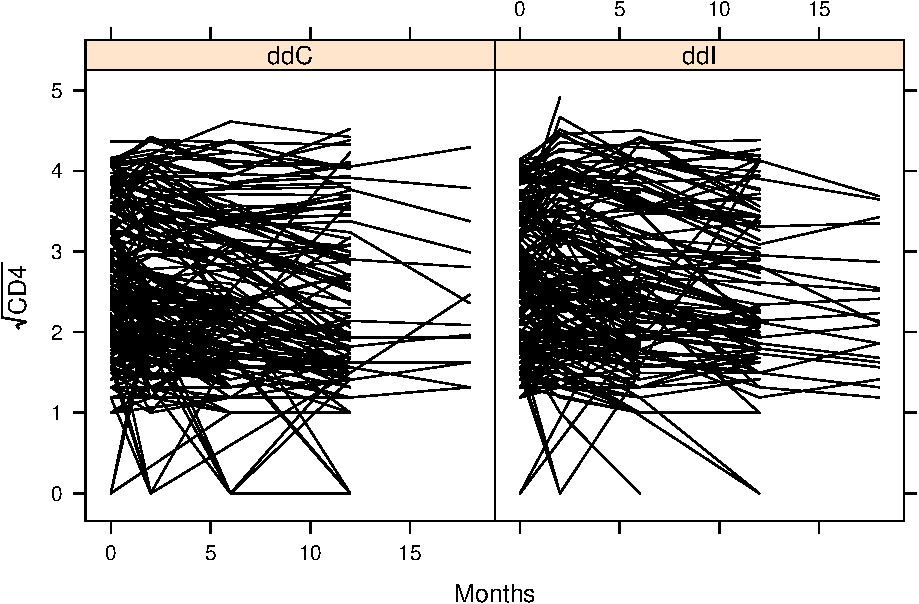
\includegraphics{bookdown_files/figure-latex/unnamed-chunk-57-1.pdf}

\begin{Shaded}
\begin{Highlighting}[]


\NormalTok{lattice}\OperatorTok{::}\KeywordTok{xyplot}\NormalTok{(}\KeywordTok{sqrt}\NormalTok{(CD4) }\OperatorTok{~}\StringTok{ }\NormalTok{obstime }\OperatorTok{|}\StringTok{ }\NormalTok{patient, }\DataTypeTok{group =}\NormalTok{ patient, }
       \DataTypeTok{data =}\NormalTok{ aids[aids}\OperatorTok{$}\NormalTok{patient }\OperatorTok\StringTok{ }\KeywordTok{c}\NormalTok{(}\DecValTok{1}\OperatorTok{:}\DecValTok{10}\NormalTok{),], }
       \DataTypeTok{xlab =} \StringTok{"Months"}\NormalTok{, }\DataTypeTok{ylab =} \KeywordTok{expression}\NormalTok{(}\KeywordTok{sqrt}\NormalTok{(}\StringTok{"CD4"}\NormalTok{)), }\DataTypeTok{col =} \DecValTok{1}\NormalTok{, }\DataTypeTok{type =} \StringTok{"b"}\NormalTok{)}
\end{Highlighting}
\end{Shaded}

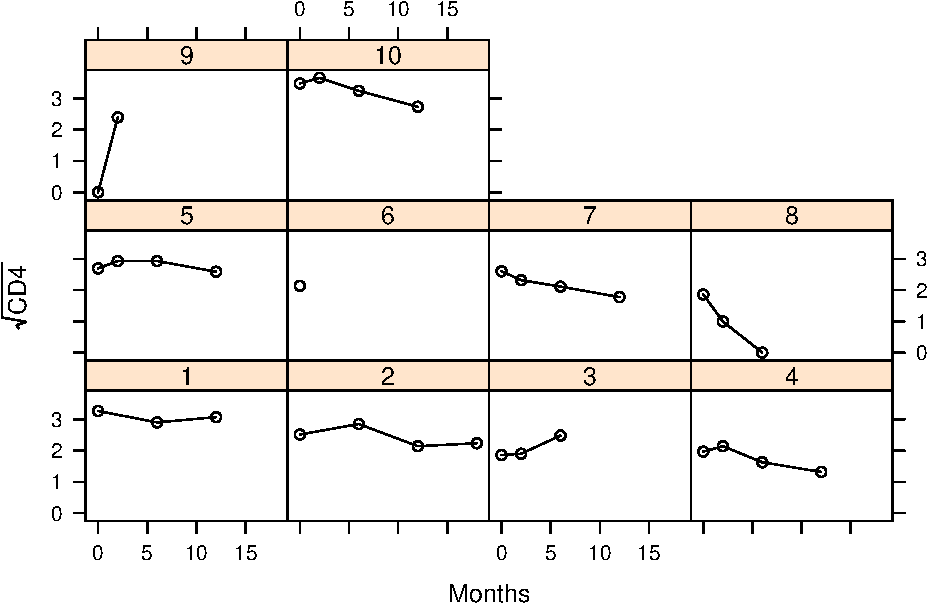
\includegraphics{bookdown_files/figure-latex/unnamed-chunk-57-2.pdf}

Now we are going to specify and fit a joint model. The linear mixed
effects model for the CD4 cell counts include:

\begin{itemize}
\tightlist
\item
  Fixed-effects part: main effect of time and the interaction with the
  treatment.
\item
  random-effects design matrix: an intercept and a time term.
\end{itemize}

The survival submodel include: treatment effect (as a time-independent
covariate) and the true underlying effect of CD4 cell count as estimated
from the longitudinal model (as time-dependent). The baseline risk
function is assumed piecewise constant.

\begin{Shaded}
\begin{Highlighting}[]
\NormalTok{fitLME <-}\StringTok{ }\KeywordTok{lme}\NormalTok{(}\KeywordTok{sqrt}\NormalTok{(CD4) }\OperatorTok{~}\StringTok{ }\NormalTok{obstime }\OperatorTok{:}\StringTok{ }\NormalTok{drug, }\DataTypeTok{random =} \OperatorTok{~}\StringTok{ }\NormalTok{obstime }\OperatorTok{|}\StringTok{ }\NormalTok{patient, }\DataTypeTok{data =}\NormalTok{ aids)}
\NormalTok{fitSURV <-}\StringTok{ }\KeywordTok{coxph}\NormalTok{(}\KeywordTok{Surv}\NormalTok{(Time, death) }\OperatorTok{~}\StringTok{ }\NormalTok{drug, }\DataTypeTok{data =}\NormalTok{ aids.id, }\DataTypeTok{x =} \OtherTok{TRUE}\NormalTok{)}
\NormalTok{fitJM <-}\StringTok{ }\KeywordTok{jointModel}\NormalTok{(fitLME, fitSURV, }\DataTypeTok{timeVar =} \StringTok{"obstime"}\NormalTok{, }\DataTypeTok{method =} \StringTok{"piecewise-PH-GH"}\NormalTok{)}
\KeywordTok{summary}\NormalTok{(fitJM)}
\NormalTok{## }
\NormalTok{## Call:}
\NormalTok{## jointModel(lmeObject = fitLME, survObject = fitSURV, timeVar = "obstime", }
\NormalTok{##     method = "piecewise-PH-GH")}
\NormalTok{## }
\NormalTok{## Data Descriptives:}
\NormalTok{## Longitudinal Process     Event Process}
\NormalTok{## Number of Observations: 1405 Number of Events: 188 (40.3%)}
\NormalTok{## Number of Groups: 467}
\NormalTok{## }
\NormalTok{## Joint Model Summary:}
\NormalTok{## Longitudinal Process: Linear mixed-effects model}
\NormalTok{## Event Process: Relative risk model with piecewise-constant}
\NormalTok{##      baseline risk function}
\NormalTok{## Parameterization: Time-dependent }
\NormalTok{## }
\NormalTok{##    log.Lik      AIC      BIC}
\NormalTok{##  -2107.647 4247.295 4313.636}
\NormalTok{## }
\NormalTok{## Variance Components:}
\NormalTok{##              StdDev    Corr}
\NormalTok{## (Intercept)  0.8660  (Intr)}
\NormalTok{## obstime      0.0388  0.0680}
\NormalTok{## Residual     0.3754        }
\NormalTok{## }
\NormalTok{## Coefficients:}
\NormalTok{## Longitudinal Process}
\NormalTok{##                   Value Std.Err z-value p-value}
\NormalTok{## (Intercept)      2.5558  0.0372 68.7961 <0.0001}
\NormalTok{## obstime:drugddC -0.0423  0.0046 -9.1931 <0.0001}
\NormalTok{## obstime:drugddI -0.0372  0.0050 -7.4577 <0.0001}
\NormalTok{## }
\NormalTok{## Event Process}
\NormalTok{##             Value Std.Err z-value p-value}
\NormalTok{## drugddI    0.3511  0.1537  2.2839  0.0224}
\NormalTok{## Assoct    -1.1016  0.1180 -9.3388 <0.0001}
\NormalTok{## log(xi.1) -1.6489  0.2498 -6.6000        }
\NormalTok{## log(xi.2) -1.3393  0.2394 -5.5940        }
\NormalTok{## log(xi.3) -1.0231  0.2861 -3.5758        }
\NormalTok{## log(xi.4) -1.5802  0.3736 -4.2299        }
\NormalTok{## log(xi.5) -1.4722  0.3500 -4.2069        }
\NormalTok{## log(xi.6) -1.4383  0.4283 -3.3584        }
\NormalTok{## log(xi.7) -1.4780  0.5455 -2.7094        }
\NormalTok{## }
\NormalTok{## Integration:}
\NormalTok{## method: Gauss-Hermite}
\NormalTok{## quadrature points: 15 }
\NormalTok{## }
\NormalTok{## Optimization:}
\NormalTok{## Convergence: 0}
\end{Highlighting}
\end{Shaded}

\BeginKnitrBlock{rmdhint_sestelo}
Remember that, due to the fact that the \texttt{jointModel} function
extracts all the required information from these two objects (e.g.,
response vectors, design matrices, etc.), in the call to the
\texttt{coxph} function we need to specify the argument
\texttt{x\ =\ TRUE}. With this, the design matrix of the Cox model is
included in the returned object.

Additionally, the main argument \texttt{timeVar} of \texttt{jointModel}
function is used to specify the name of the time variable in the linear
mixed effects model, which is required for the computation of
\(m_i(t)\).
\EndKnitrBlock{rmdhint_sestelo}

Note that in the results of the event process the parameter labeled
\texttt{Assoct} is the parameter \(\alpha\) in the equation
\eqref{eq:joint} that measures the effect of \(m_i(t)\) (i.e., in our case
of the true square root CD4 cell count) in the risk for death. The
parameters \(x_i\) are the parameters for the piecewise constant
baseline risk function. As we can see there is a significant effect of
longitudinal outcome on the risk. For obtaining the Hazard Ratio for
this variable we have to exponenciate the value exposed in the table. In
this case the result is 0.33. According to this, one unit increse on the
CD4 count cell decreases the risk 67\%.

If we want to test for a treatment effect, an alternative to the Wald
test with a pvalue around 0.03, is the Likelihood Ratio Test (LRT). To
perform it we need to fit the joint model under the null hypothesis of
no treatment effect in the survival submodel, and then use the
\texttt{anova} function

\begin{Shaded}
\begin{Highlighting}[]
\NormalTok{fitSURV2 <-}\StringTok{ }\KeywordTok{coxph}\NormalTok{(}\KeywordTok{Surv}\NormalTok{(Time, death) }\OperatorTok{~}\StringTok{ }\DecValTok{1}\NormalTok{, }\DataTypeTok{data =}\NormalTok{ aids.id, }\DataTypeTok{x =} \OtherTok{TRUE}\NormalTok{)}
\NormalTok{fitJM2 <-}\StringTok{ }\KeywordTok{jointModel}\NormalTok{(fitLME, fitSURV2, }\DataTypeTok{timeVar =} \StringTok{"obstime"}\NormalTok{, }\DataTypeTok{method =} \StringTok{"piecewise-PH-GH"}\NormalTok{)}
\KeywordTok{anova}\NormalTok{(fitJM2, fitJM) }\CommentTok{# the model under the null is the first one}
\NormalTok{## }
\NormalTok{##            AIC     BIC  log.Lik  LRT df p.value}
\NormalTok{## fitJM2 4250.53 4312.72 -2110.26                }
\NormalTok{## fitJM  4247.29 4313.64 -2107.65 5.23  1  0.0222}
\end{Highlighting}
\end{Shaded}

According to the pvalue (as with the Wald test) we arrive to the same
conclusion, there exist an affect of the treatment on the risk.

Additionally, if we want to obtain \textbf{estimates of the Hazard Ratio
with confidence intervals} for the final model it is possible ti apply
the \texttt{confint} function to the created object

\begin{Shaded}
\begin{Highlighting}[]
\KeywordTok{confint}\NormalTok{(fitJM, }\DataTypeTok{parm =} \StringTok{"Event"}\NormalTok{)}
\NormalTok{##               2.5 %       est.     97.5 %}
\NormalTok{## drugddI  0.04979688  0.3511323  0.6524677}
\NormalTok{## Assoct  -1.33281297 -1.1016129 -0.8704128}
\KeywordTok{exp}\NormalTok{(}\KeywordTok{confint}\NormalTok{(fitJM, }\DataTypeTok{parm =} \StringTok{"Event"}\NormalTok{))}
\NormalTok{##             2.5 %      est.    97.5 %}
\NormalTok{## drugddI 1.0510576 1.4206752 1.9202736}
\NormalTok{## Assoct  0.2637343 0.3323346 0.4187786}
\end{Highlighting}
\end{Shaded}

Finally, we will focus on the calculation of \textbf{expected survival
probabilities}. For this we have to use the \texttt{survfitJM} function
that accepts as main arguments a fitted joint model, and a data frame
that contains the longitudinal and covariate information for the
subjects for which we wish to calculate the predicted survival
probabilities.

Here we compute the expected survival probabilies for two patients in
the data set who \textbf{has not died} by the time of loss to follow-up.
The function assumes that the patient has survived up to the last time
point \(t\) in newdata for which a CD4 measurement was recorded, and
will produce survival probabilities for a set of predefined \(u > t\)
values

\begin{Shaded}
\begin{Highlighting}[]
\KeywordTok{set.seed}\NormalTok{(}\DecValTok{300716}\NormalTok{) }\CommentTok{# it uses Monte Carlo samples}
\NormalTok{preds <-}\StringTok{ }\KeywordTok{survfitJM}\NormalTok{(fitJM, }\DataTypeTok{newdata =}\NormalTok{ aids[aids}\OperatorTok{$}\NormalTok{patient }\OperatorTok\StringTok{ }\KeywordTok{c}\NormalTok{(}\StringTok{"7"}\NormalTok{, }\StringTok{"15"}\NormalTok{), ],}
          \DataTypeTok{idVar =} \StringTok{"patient"}\NormalTok{)  }\CommentTok{# last.time = "Time"}

\KeywordTok{survfitJM}\NormalTok{(fitJM, }\DataTypeTok{newdata =}\NormalTok{ aids[aids}\OperatorTok{$}\NormalTok{patient }\OperatorTok\StringTok{ }\KeywordTok{c}\NormalTok{(}\StringTok{"7"}\NormalTok{, }\StringTok{"15"}\NormalTok{), ], }\DataTypeTok{idVar =} \StringTok{"patient"}\NormalTok{, }
          \DataTypeTok{survTimes =} \KeywordTok{c}\NormalTok{(}\DecValTok{20}\NormalTok{, }\DecValTok{30}\NormalTok{, }\DecValTok{40}\NormalTok{))  }\CommentTok{# you can specify the times}
\NormalTok{## }
\NormalTok{## Prediction of Conditional Probabilities for Event}
\NormalTok{##  based on 200 Monte Carlo samples}
\NormalTok{## }
\NormalTok{## $`7`}
\NormalTok{##   times   Mean Median  Lower  Upper}
\NormalTok{## 1    12 1.0000 1.0000 1.0000 1.0000}
\NormalTok{## 1    20 0.7048 0.7165 0.4336 0.8900}
\NormalTok{## 2    30 0.3810 0.3872 0.0167 0.7936}
\NormalTok{## 3    40 0.1859 0.1173 0.0000 0.6969}
\NormalTok{## }
\NormalTok{## $`15`}
\NormalTok{##   times   Mean Median  Lower  Upper}
\NormalTok{## 1    12 1.0000 1.0000 1.0000 1.0000}
\NormalTok{## 1    20 0.8663 0.8704 0.7360 0.9588}
\NormalTok{## 2    30 0.6826 0.7103 0.2408 0.9320}
\NormalTok{## 3    40 0.5076 0.5271 0.0386 0.9116}
\end{Highlighting}
\end{Shaded}

Note that the first time of the output is the last time observed in the
longitudinal study. This is because for the time points that are earlier
than this time we know that this subject was alive and therefore
survival probability is 1.

\begin{Shaded}
\begin{Highlighting}[]
\KeywordTok{par}\NormalTok{(}\DataTypeTok{mfrow=}\KeywordTok{c}\NormalTok{(}\DecValTok{1}\NormalTok{,}\DecValTok{2}\NormalTok{))}
\KeywordTok{plot}\NormalTok{(preds, }\DataTypeTok{which =} \StringTok{"7"}\NormalTok{, }\DataTypeTok{conf.int =} \OtherTok{TRUE}\NormalTok{)}

\KeywordTok{plot}\NormalTok{(preds, }\DataTypeTok{which =} \StringTok{"7"}\NormalTok{, }\DataTypeTok{conf.int =} \OtherTok{TRUE}\NormalTok{, }
     \DataTypeTok{fun =} \ControlFlowTok{function}\NormalTok{ (x) }\OperatorTok{-}\KeywordTok{log}\NormalTok{(x), }\DataTypeTok{ylab =} \StringTok{"Cumulative Risk"}\NormalTok{)}
\end{Highlighting}
\end{Shaded}

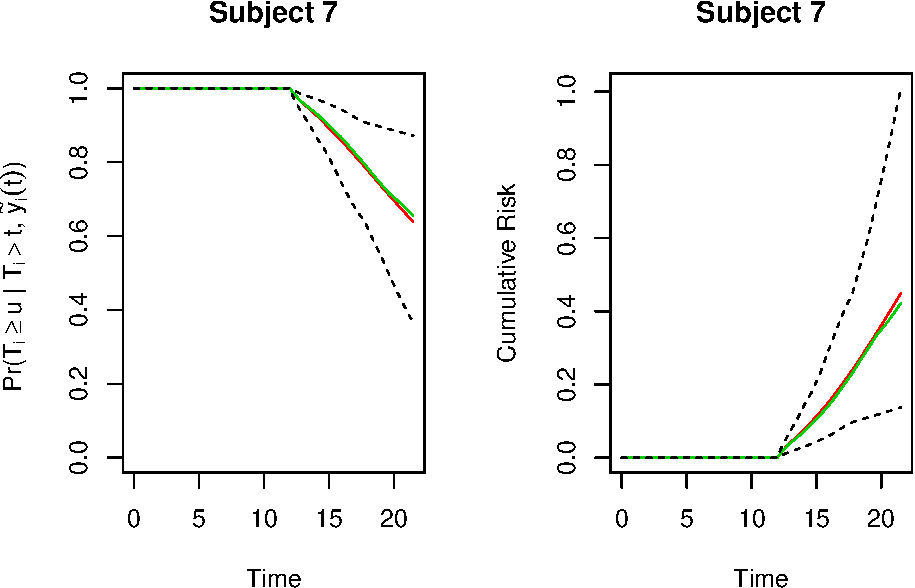
\includegraphics{bookdown_files/figure-latex/unnamed-chunk-63-1.pdf}

\chapter{\texorpdfstring{Conditinal Survival with
\texttt{condSURV}}{Conditinal Survival with condSURV}}\label{condsurv}

In this chapter we will see the estimation of the survival function when
we have ordered multivariate failure time data. This estimation will be
obtained by means of the \texttt{condSURV} package, which provides three
different approaches all based on the Kaplan-Meier estimator.

\section{Introduction}\label{introduction}

As we saw, the \textbf{most popular} method for estimating survival,
when there is censoring, is the well-known product-limit estimator also
known as \textbf{Kaplan-Meier estimator} \citep{KM58}. The popularity of
the product-limit estimator is explained by its simplicity and intuitive
appeal while requiring very week assumptions. It simply takes into
account with the empirical probability of surviving over certain time.

\textbf{The method does not take into account of covariates}, so it is
mainly descriptive. Discrete covariates can be included by splitting the
sample for each level of the covariate and applying the product-limit
estimator for each subsample. This approach is not recommended for
continuous covariates.

To account to this extra difficulty several generalizations to the
Kaplan-Meier estimator have been proposed throughout the last decades.
\citet{Beran81} was the first one who proposed an estimator of the
conditional distribution (survival) function with censored data in a
fully nonparametric way. His estimator was further studied among others
by \citet{Dabrowska87}, \citet{Akritas94}, \citet{Manteiga94} and
\citet{VanKeilegom2001}. All these estimators can be used to estimate
the distribution (or survival) function conditional to a continuous
covariable in a regression model, when data are subject to censoring.
However, \textbf{none of the above} methods can be used to estimate the
conditional survival when \textbf{the covariate is censored}.

In many longitudinal medical studies, patients may experience
\textbf{several events} through a follow-up period. In these studies,
the analysis of sequentially ordered events are often of interest. The
events of concern can be of the same nature (e.g., recurrent disease
episodes in cancer studies) or represent different states in the disease
process (e.g., `alive and disease-free', `alive with recurrence' and
`dead'). If the events are of the same nature, this is usually referred
as \textbf{recurrent events} \citep{Cook}. One example of this scheme
can be see at Figure \ref{fig:image}.

\begin{figure}

{\centering 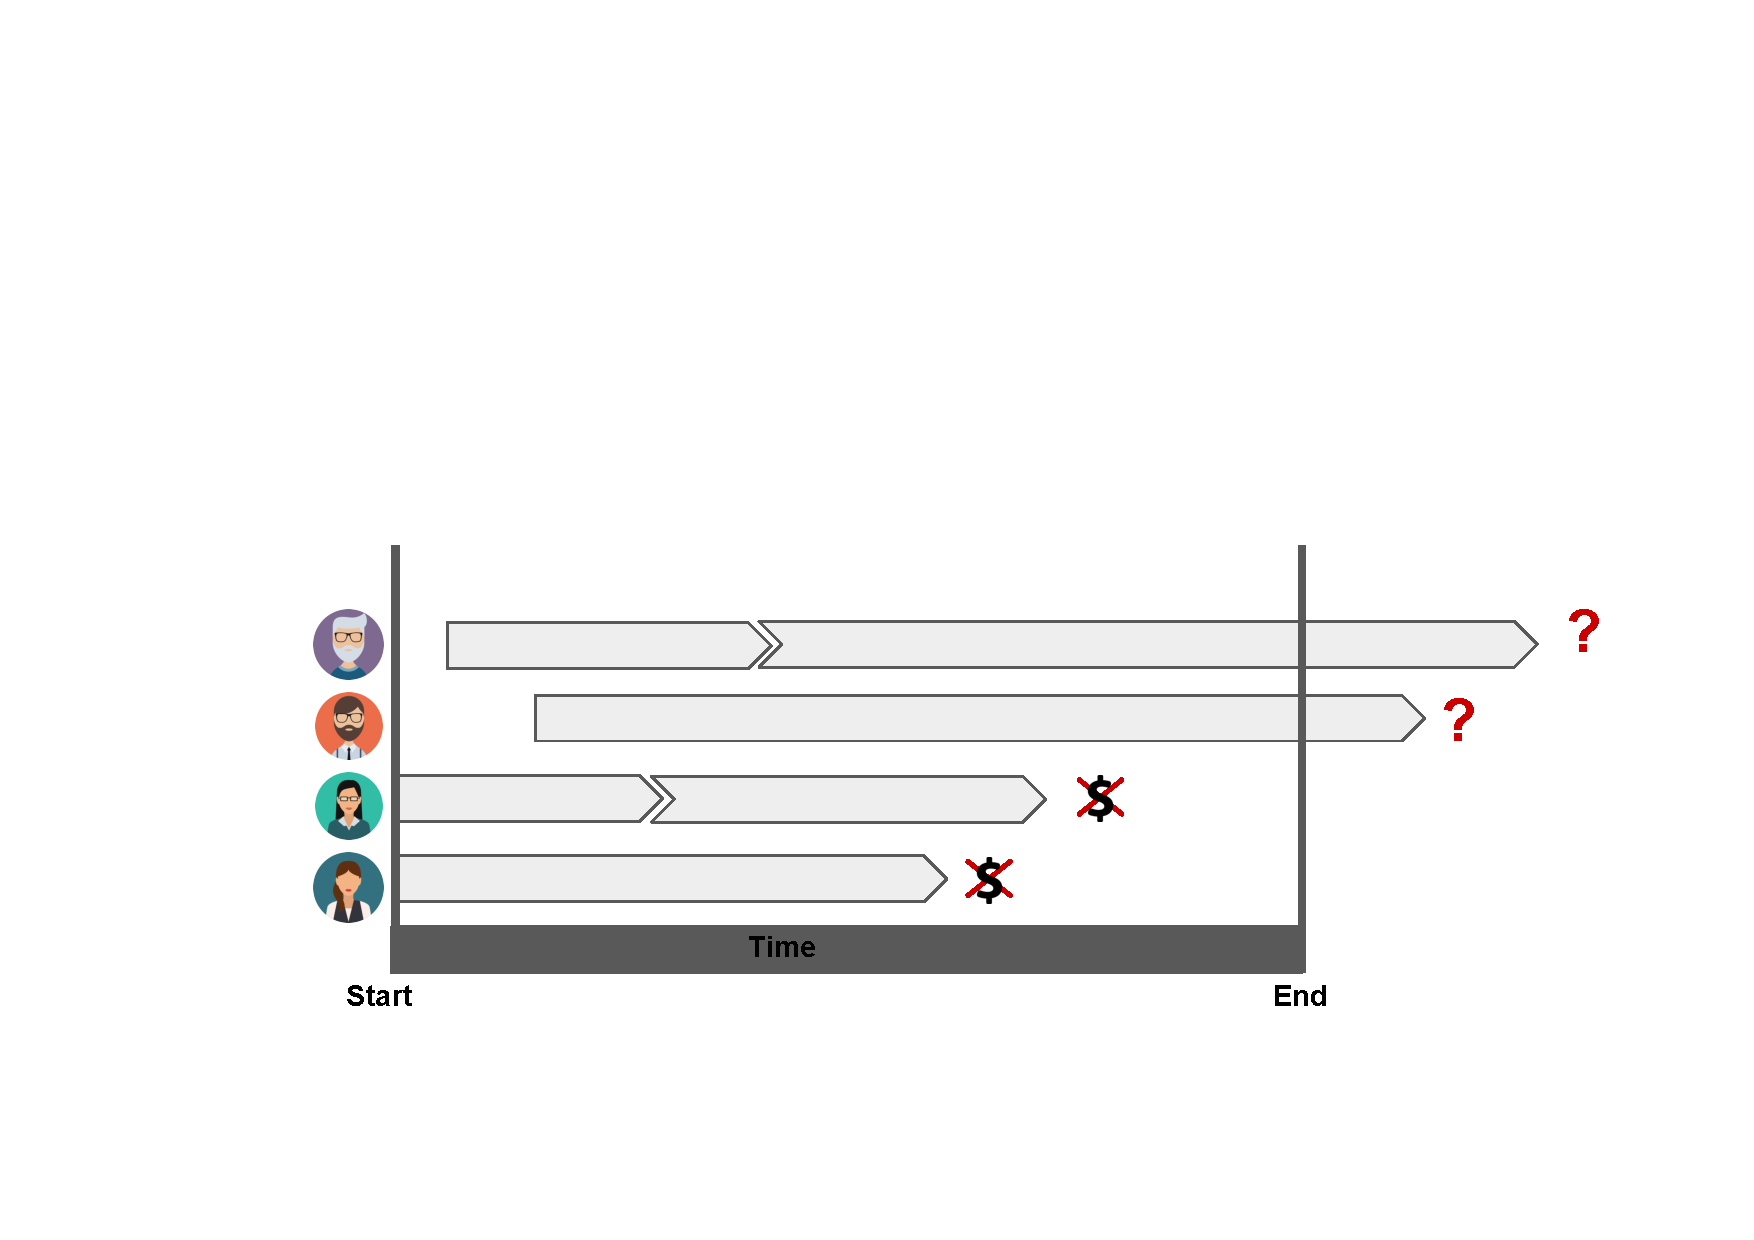
\includegraphics{images/saBBVA_recurrence} 

}

\caption{Illustration of censoring.}\label{fig:image}
\end{figure}

In the above situation maybe we want to obtain estimates for some
conditional survival. Let's do it now!

\section{Notation}\label{notation}

Suppose that an individual may experience \(K\) consecutive events at
times \(T_1<T_2<\cdot\cdot\cdot<T_K=T\), which are measured from the
start of the follow-up.

Here different methods are proposed to estimate \textbf{conditional
survival probabilities} such as \(P(T_2 > y \mid T_1 > x)\) or
\(P(T_2 > y \mid T_1 \leq x)\), where \(T_1\) and \(T_2\) are ordered
event times of two successive events.

The proposed methods are all \textbf{based on the Kaplan-Meier}
estimator and the ideas behind the proposed estimators can also be used
to estimate more general functions involving \textbf{more than two
successive event times}. However, for ease of presentation and without
loss of generality, we take \(K=2\) in this section. The extension to
\(K>2\) is straightforward.

\begin{figure}

{\centering 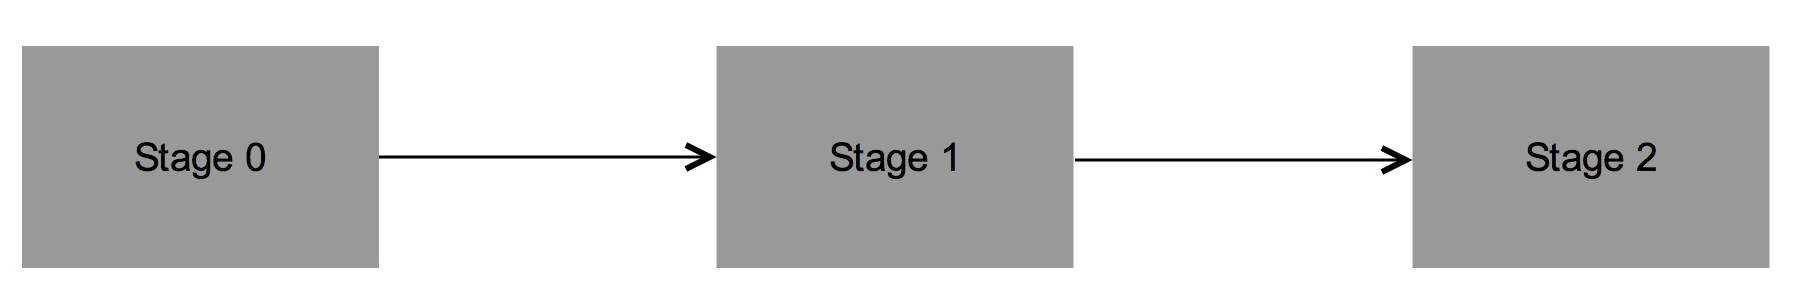
\includegraphics{images/stage3box} 

}

\caption{3-state progresive model.}\label{fig:progres}
\end{figure}

Let \((T_{1},T_{2})\) be a pair of successive event times corresponding
to two ordered (possibly consecutive) events measured from the start of
the follow-up.

Let \(T=T_{2}\) denote the total time and assume that both \(T_1\) and
\(T\) are observed subject to a (univariate) random right-censoring
variable \(C\) assumed to be independent of \((T_1,T)\). Due to
censoring, rather than \((T_1,T)\) we observe
\((\widetilde T_{1},\Delta_1,\widetilde T,\Delta_2)\) where
\(\widetilde T_{1}=\min (T_{1},C)\), \(\Delta_{1}=I(T_{1}\leq C)\),
\(\widetilde T=\min (T,C)\), \(\Delta_{2}=I(T\leq C)\), where
\(I(\cdot)\) is the indicator function. Let
\((\widetilde T_{1i},\Delta_{1i},\widetilde T_i,\Delta_{2i})\),
\(1\leq i\leq n\) be independent and identically distributed data with
the same distribution as
\((\widetilde T_{1},\Delta_1,\widetilde T,\Delta_2)\).

\section{Estimation of the conditional
survival}\label{estimation-of-the-conditional-survival}

Let \(S_1\) and \(S\) be the marginal survival functions of \(T_1\) and
\(T\); that is, \(S_1(y)=P(T_1>y)\) and \(S(y)=P(T>y)\). Introduce also
the conditional survival probabilities \(P(T>y|T_1>x)\) and
\(P(T>y|T_1\leq x)\). without loss of generality, we only consider the
estimation of \(S(y|x)=P(T>y|T_1>x)\).

The Kaplan-Meier estimator, also known as the product-limit estimator,
is the most frequently used method to estimate survival for censored
data. The most used representation of the Kaplan-Meier estimator of the
total time is through a product of the following form

\begin{eqnarray*}
\widehat S(y)=\prod_{\widetilde T_i\leq t}\left(1-\frac{\Delta_{2i}}{R(\widetilde T_i)}\right)
\end{eqnarray*}

\noindent where \(R(t)=\sum_{i=1}^{n} I(\widetilde T_i \geq t)\) denote
the number of individuals at risk just before time \(t\).

Below we introduce a weighted average representation of the Kaplan-Meier
estimator which will be used later to introduce estimators for the
conditional survival function

\begin{equation*}
\widehat S(y)=1-\sum_{i=1}^{n}W_{i}I(\widetilde T_{(i)}\leq y),%\equiv 1-\widehat{F}_1(x),
\end{equation*}

\noindent where
\(\widetilde T_{\left( 1\right) }\leq ...\leq \widetilde T_{\left( n\right) }\)
denotes the ordered \(\widetilde T\)-sample and

\begin{equation*}
W_{i}=\frac{\Delta_{2\left[ i\right] }}{n-i+1}\prod_{j=1}^{i-1}\left[ 1-\frac{%
\Delta _{2\left[ j\right] }}{n-j+1}\right]
\end{equation*}

\noindent is the Kaplan-Meier weight attached to
\(\widetilde T_{\left( i\right) }\). In the expression of \(W_{i}\)
notation \(\Delta_{2\left[ i\right] }\) is used for the \(i\)-th
concomitant value of the censoring indicator (that is,
\(\Delta_{2\left[ i \right] }=\Delta _{2j}\) if
\(\widetilde T_{\left( i\right) }=\widetilde T_{j}\)).

Well, we are interested in the estimation of the \textbf{conditional
survival function, \(S(y\mid x)=P(T>y\mid T_1>x)\)}. Below we provide
estimators for this quantity, all based on the Kaplan-Meier estimator.

\subsection{\texorpdfstring{Kaplan-Meier Weighted Estimator
(\texttt{KMW})}{Kaplan-Meier Weighted Estimator (KMW)}}\label{kaplan-meier-weighted-estimator-kmw}

Since \(S(y\mid x)\) can be expressed as
\(S(y\mid x)=P(T > y|T_1 > x) = 1 - P(T\leq y\mid T_1 > x)= 1 - P(T_1 > x, T\leq y)/\left(1-P\left(T_1\leq x\right)\right),\)
the conditional survival function may be estimated as

\begin{equation}
\widehat S^{\texttt{KMW}}(y\mid x)=1-\frac{\sum_{i=1}^{n}{W_iI(\widetilde T_{1\left[i\right]} >x, \widetilde T_{\left(i\right)} \leq y)}}{\widehat S_1(x)}.
\end{equation}

\subsection{\texorpdfstring{The Landmark approach
(\texttt{LDM})}{The Landmark approach (LDM)}}\label{the-landmark-approach-ldm}

The Landmark approach \citep{vanHouwelingen} states that, given the time
point \(x\), to estimate \(S(y\mid x)=P(T> y\mid T_1>x)\) the analysis
can be restricted to the individuals with an observed first event time
greater than \(x\).

Let \(n_x\) be the cardinal of \(\left\{i:\widetilde T_{1i}>x\right\}\)
and
\(\left( \widetilde T_{\left( i\right) }^{x},\Delta_{\left[ i\right]}^{x}\right)\),
\(i=1,...,n_{x}\), is the \(\left(\widetilde T,\Delta\right)\)-sample in
\(\left\{i:\widetilde T_{1i}>x\right\}\)~ordered with respect to
\(\widetilde T\).

\begin{equation*}
\widehat S^{\texttt{LDM}}(y\mid x)=1-\sum_{i=1}^{n_x}{W_i^{x}I(\widetilde T_{\left(i\right)}^x \leq y)}.
\end{equation*}

\noindent where \(W_i^{x}\) denotes the Kaplan-Meier weight attached to
the i-th ordered T-datum, computed from the subsample
\(\left\{i:\widetilde T_{1i}>x\right\}\).

\subsection{\texorpdfstring{The Presmoothed Landmark approach
(\texttt{PLDM})}{The Presmoothed Landmark approach (PLDM)}}\label{the-presmoothed-landmark-approach-pldm}

The standard error of the LDM approach may be large when the censoring
is heavy, particularly with a small sample size. Interestingly, the
variance of this estimator may be reduced by presmoothing
\citep{Dikta1998}. Here, the idea of presmoothing involves replacing the
censoring indicators (in the expression of the Kaplan-Meier weights) by
some smooth fit before the Kaplan-Meier formula is applied. This
preliminary smoothing may be based on a certain parametric family such
as the logistic (thus leading to a semiparametric estimator), or on a
nonparametric estimator of the binary regression curve. The
corresponding presmoothed landmark estimator is then given by

\begin{equation*}
\widehat S^{\texttt{PDLM}}(y\mid x)=1-\sum_{i=1}^{n_x}{W_i^{x\star}I(\widetilde T_{\left(i\right)}^x \leq y)}
\end{equation*}

\noindent where \(W_{i}^{x\star}\) is defined through

\begin{equation*}
    W_{i}^{x\star}=\frac {m(\widetilde T_{\left(i\right)}^{x})}{n_x-i+1}\prod_{j=1}^{i-1}\left[1-\frac {m(\widetilde T_{\left(j\right)}^{x})}{n_x-j+1}\right], \quad 1\leq i\leq n_{x},
\end{equation*}

\noindent where
\(\left( \widetilde T_{\left( i\right) }^{x},\Delta_{\left[ i\right]}^{x}\right)\),
\(i=1,...,n_{x}\), is the \(\left( \widetilde T,\Delta\right)\)-sample
in \(\left\{i:\widetilde T_{1i}>x\right\}\)~ordered with respect to
\(\widetilde T\).

Here, \(m(t)= P(\Delta=1\mid \widetilde T^{x}=t)\).
\(m(\widetilde T^{x})\) belongs to a parametric (smooth) family of
binary regression curves, e.g., logistic.

According to the performance, it has been demonstrated that \textbf{all
of the estimators perform well}, approaching their targets as the sample
size increases. Besides, simulation results reveal that the landmark
estimator (\texttt{LDM}) perform favorably when compared with the first
method (\texttt{KMW}). Furthermore, the reported simulation results
reveal relative benefits of presmoothing (\texttt{PLDM}) in the heavily
censored scenarios or small sample sizes.

\section{\texorpdfstring{The \texttt{condSURV}
package}{The condSURV package}}\label{the-condsurv-package}

To illustrate our methods we will use data from a German Breast cancer
study \citep{book:1506027}. This data set is freely available as part of
the `condSURV package.

In this dataset, a total of 686 woman with primary node positive Breast
cancer were recruited in the period between 1984 and 1989. From this
total, 299 developed a recurrence and among these 171 died.

For each patient, the two event times (time to recurrence and time to
death) and the corresponding indicator status is recorded. Other
covariates were also recorded. The covariate \texttt{recurrence} is the
only time-dependent covariate, while the other covariates included are
fixed. Recurrence can be considered as an intermediate transient state
and modeled using a three-state progressive model with states
\textbf{Alive and disease-free}, \textbf{Alive with Recurrence} and
\textbf{Dead}. You can see an example at Figure \ref{fig:breast}.

The effect of \texttt{recurrence} is important on the patient outcome
and can be studied through the ordered multivariate event time data of
time-to-event from enrollment, to recurrence and to death. Results
obtained from the estimation of the conditional survival probabilities,
\(S(y\mid x)=P(T>y|T_1>x)\), can be used to understand which individuals
without recurring cancer after surgery are most likely to survive from
their disease and which would benefit from more personal attention,
closer follow-up and monitoring.

\begin{figure}

{\centering 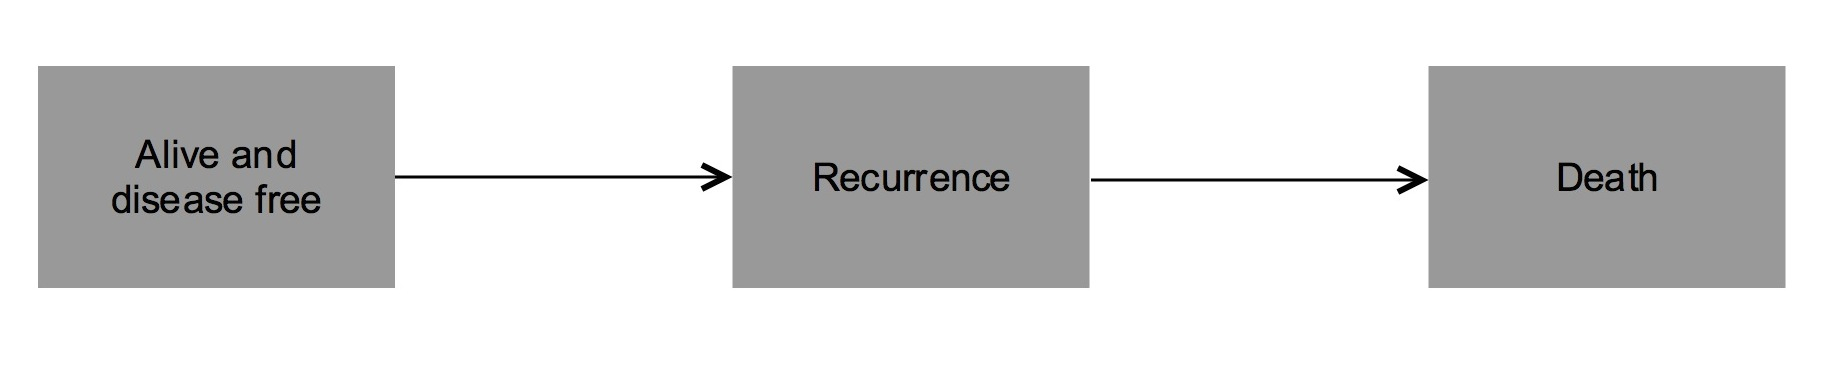
\includegraphics{images/alive3box} 

}

\caption{Scheme of the model.}\label{fig:breast}
\end{figure}

Bellow is an excerpt of the data.frame with one row per individual

\begin{Shaded}
\begin{Highlighting}[]
\KeywordTok{head}\NormalTok{(gbcsCS)}
\NormalTok{##   id  diagdateb    recdate  deathdate age menopause hormone size grade}
\NormalTok{## 1  1 17-08-1984 15-04-1988 16-11-1990  38         1       1   18     3}
\NormalTok{## 2  2 25-04-1985 15-03-1989 22-10-1990  52         1       1   20     1}
\NormalTok{## 3  3 11-10-1984 12-04-1988 06-10-1988  47         1       1   30     2}
\NormalTok{## 4  4 29-06-1984 24-11-1984 24-11-1984  40         1       1   24     1}
\NormalTok{## 5  5 03-07-1984 09-08-1989 09-08-1989  64         2       2   19     2}
\NormalTok{## 6  6 24-07-1984 08-11-1989 08-11-1989  49         2       2   56     1}
\NormalTok{##   nodes prog_recp estrg_recp rectime censrec survtime censdead}
\NormalTok{## 1     5       141        105    1337       1     2282        0}
\NormalTok{## 2     1        78         14    1420       1     2006        0}
\NormalTok{## 3     1       422         89    1279       1     1456        1}
\NormalTok{## 4     3        25         11     148       0      148        0}
\NormalTok{## 5     1        19          9    1863       0     1863        0}
\NormalTok{## 6     3       356         64    1933       0     1933        0}

\NormalTok{kmw1 <-}\StringTok{ }\KeywordTok{survCOND}\NormalTok{(}\KeywordTok{survCS}\NormalTok{(rectime, censrec, survtime, censdead) }\OperatorTok{~}\StringTok{ }\DecValTok{1}\NormalTok{,}
\DataTypeTok{x =} \DecValTok{365}\NormalTok{, }\DataTypeTok{y =} \DecValTok{1460}\NormalTok{, }\DataTypeTok{data =}\NormalTok{ gbcsCS, }\DataTypeTok{method =} \StringTok{"KMW"}\NormalTok{, }\DataTypeTok{conf =} \OtherTok{TRUE}\NormalTok{, }\DataTypeTok{n.boot =} \DecValTok{100}\NormalTok{)}

\KeywordTok{summary}\NormalTok{(kmw1)}
\NormalTok{## }
\NormalTok{## P(T>y|T1>365) }
\NormalTok{## }
\NormalTok{##     y  estimate lower 95% CI upper 95% CI}
\NormalTok{##  1460 0.8050317    0.7660963    0.8406652}
\end{Highlighting}
\end{Shaded}

With the previous code you can obtain the estimates for the probability
that a woman survives more than four years given that she is alive and
disease-free at one year after the surgery. Note that the package
contains the function \texttt{survCS} which takes the input data as an
\texttt{R} formula and creates a survival object among the chosen
variables for analysis. This function will verify if the data has been
introduced correctly and create a \texttt{survCS} object. Arguments in
this function must be introduced in the following order \texttt{time1},
\texttt{event1}, \texttt{time2}, \texttt{event2},\ldots{},
\texttt{Stime} and \texttt{event}, where \texttt{time1}, \texttt{time2},
\ldots{}, \texttt{Stime} are ordered event times and \texttt{event1},
\texttt{event2},\ldots{}, \texttt{event} their corresponding indicator
statuses. This function plays a similar role as the \texttt{Surv}
function in the \texttt{survival} package.

\begin{Shaded}
\begin{Highlighting}[]
\CommentTok{# including more times}
\NormalTok{kmw2 <-}\StringTok{ }\KeywordTok{survCOND}\NormalTok{(}\KeywordTok{survCS}\NormalTok{(rectime, censrec, survtime, censdead) }\OperatorTok{~}\StringTok{ }\DecValTok{1}\NormalTok{,}
\DataTypeTok{x =} \DecValTok{365}\NormalTok{, }\DataTypeTok{y =} \DecValTok{365} \OperatorTok{*}\StringTok{ }\DecValTok{1}\OperatorTok{:}\DecValTok{7}\NormalTok{, }\DataTypeTok{data =}\NormalTok{ gbcsCS, }\DataTypeTok{method =} \StringTok{"KMW"}\NormalTok{, }\DataTypeTok{conf =} \OtherTok{TRUE}\NormalTok{) }

\KeywordTok{summary}\NormalTok{(kmw2)}
\NormalTok{## }
\NormalTok{## P(T>y|T1>365) }
\NormalTok{## }
\NormalTok{##     y  estimate lower 95% CI upper 95% CI}
\NormalTok{##   365 1.0000000    1.0000000    1.0000000}
\NormalTok{##   730 0.9429857    0.9243627    0.9617317}
\NormalTok{##  1095 0.8805697    0.8535489    0.9086733}
\NormalTok{##  1460 0.8050317    0.7672805    0.8397826}
\NormalTok{##  1825 0.7506686    0.7107210    0.7870262}
\NormalTok{##  2190 0.6627422    0.6036218    0.7229263}
\NormalTok{##  2555 0.6205942    0.5174107    0.7037316}


\CommentTok{# with y omitted}
\NormalTok{kmw3 <-}\StringTok{ }\KeywordTok{survCOND}\NormalTok{(}\KeywordTok{survCS}\NormalTok{(rectime, censrec, survtime, censdead) }\OperatorTok{~}\StringTok{ }\DecValTok{1}\NormalTok{,}
\DataTypeTok{x =} \DecValTok{365}\NormalTok{, }\DataTypeTok{data =}\NormalTok{ gbcsCS, }\DataTypeTok{method =} \StringTok{"KMW"}\NormalTok{, }\DataTypeTok{conf =} \OtherTok{TRUE}\NormalTok{)}

\CommentTok{# note the `times` argument}
\KeywordTok{summary}\NormalTok{(kmw3, }\DataTypeTok{times =} \KeywordTok{c}\NormalTok{(}\DecValTok{730}\NormalTok{, }\DecValTok{1095}\NormalTok{))  }
\NormalTok{##     y  estimate lower 95% CI upper 95% CI}
\NormalTok{##   730 0.9429857    0.9257512    0.9594349}
\NormalTok{##  1095 0.8805697    0.8541121    0.9076813}
\end{Highlighting}
\end{Shaded}

In addition, one may also be interested in calculating the conditional
survival function, \(S(y\mid x)=P(T>y|T_1\leq x)\). This is the
probability of the individual to be alive at time \(y\) conditional that
he/she is alive with recurrence at a previous time \(x\).

\begin{Shaded}
\begin{Highlighting}[]
\CommentTok{# P(T > y | T1 < x)}
\NormalTok{kmw4 <-}\StringTok{ }\KeywordTok{survCOND}\NormalTok{(}\KeywordTok{survCS}\NormalTok{(rectime, censrec, survtime, censdead) }\OperatorTok{~}\StringTok{ }\DecValTok{1}\NormalTok{,}
\DataTypeTok{x =} \DecValTok{365}\NormalTok{, }\DataTypeTok{data =}\NormalTok{ gbcsCS, }\DataTypeTok{method =} \StringTok{"KMW"}\NormalTok{, }\DataTypeTok{conf =} \OtherTok{TRUE}\NormalTok{, }\DataTypeTok{lower.tail =} \OtherTok{TRUE}\NormalTok{) }

\KeywordTok{summary}\NormalTok{(kmw4, }\DataTypeTok{times =} \KeywordTok{c}\NormalTok{(}\DecValTok{730}\NormalTok{, }\DecValTok{1095}\NormalTok{))}
\NormalTok{##     y  estimate lower 95% CI upper 95% CI}
\NormalTok{##   730 0.3448798   0.22574983    0.4583618}
\NormalTok{##  1095 0.2165459   0.09451544    0.3168580}
\end{Highlighting}
\end{Shaded}

Similarly, one can obtain the results for the landmark methods
(\texttt{LDM} and \texttt{PLDM}) using the same function
\texttt{survCOND}. The unsmoothed landmark estimator is obtained using
argument \texttt{method\ =\ "LDM"} whereas for obtaining the presmoothed
landmark estimator the argument \texttt{presmooth\ =\ TRUE} is also
required.

\begin{Shaded}
\begin{Highlighting}[]
\KeywordTok{plot}\NormalTok{(kmw3, }\DataTypeTok{confcol =} \StringTok{"red"}\NormalTok{, }\DataTypeTok{xlab =} \StringTok{"Time (days)"}\NormalTok{, }\DataTypeTok{ylab =} \StringTok{"S(y|365)"}\NormalTok{)}
\end{Highlighting}
\end{Shaded}

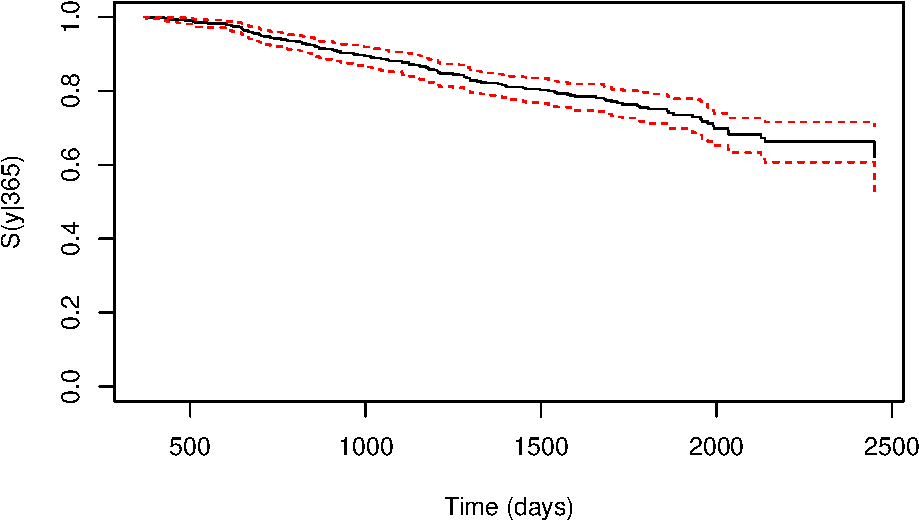
\includegraphics{bookdown_files/figure-latex/unnamed-chunk-67-1.pdf}

One important goal is to obtain estimates for the above estimated
quantities (conditional survival probabilities) conditionally on current
or past covariate measures. The current version of the package allow the
inclusion of a single covariate.

\begin{Shaded}
\begin{Highlighting}[]
\NormalTok{grade <-}\StringTok{ }\KeywordTok{survCOND}\NormalTok{(}\KeywordTok{survCS}\NormalTok{(rectime, censrec, survtime, censdead) }\OperatorTok{~}\StringTok{ }\KeywordTok{as.factor}\NormalTok{(grade),}
                  \DataTypeTok{x =} \DecValTok{365}\NormalTok{, }\DataTypeTok{data =}\NormalTok{ gbcsCS, }\DataTypeTok{method =} \StringTok{"LDM"}\NormalTok{, }\DataTypeTok{conf =} \OtherTok{FALSE}\NormalTok{)}
\KeywordTok{plot}\NormalTok{(grade)}
\end{Highlighting}
\end{Shaded}

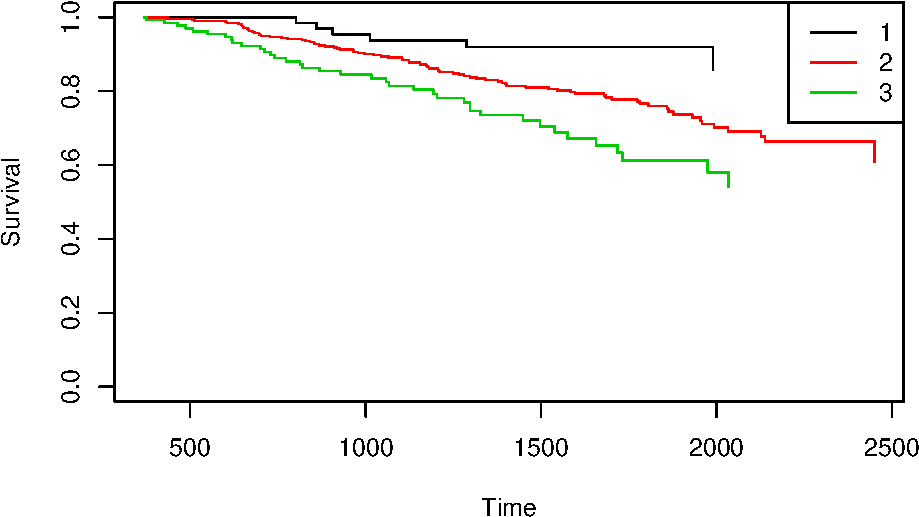
\includegraphics{bookdown_files/figure-latex/unnamed-chunk-68-1.pdf}

Finally, the package also allow the user to estimate the conditional
survival given a continuous covariate (i.e., objects of class `integer'
or `numeric'). For example, estimates and plot for the conditional
survival for women aged 60 years, \(S(y|x,Z=z)=P(T>y|T_1>x, age=60)\).

\begin{Shaded}
\begin{Highlighting}[]
\NormalTok{age <-}\StringTok{ }\KeywordTok{survCOND}\NormalTok{(}\KeywordTok{survCS}\NormalTok{(rectime, censrec, survtime, censdead) }\OperatorTok{~}\StringTok{ }\NormalTok{age, }\DataTypeTok{x =} \DecValTok{365}\NormalTok{, }
                \DataTypeTok{z.value =} \DecValTok{60}\NormalTok{, }\DataTypeTok{data =}\NormalTok{ gbcsCS, }\DataTypeTok{conf =} \OtherTok{FALSE}\NormalTok{)}
\KeywordTok{plot}\NormalTok{(age)}
\end{Highlighting}
\end{Shaded}

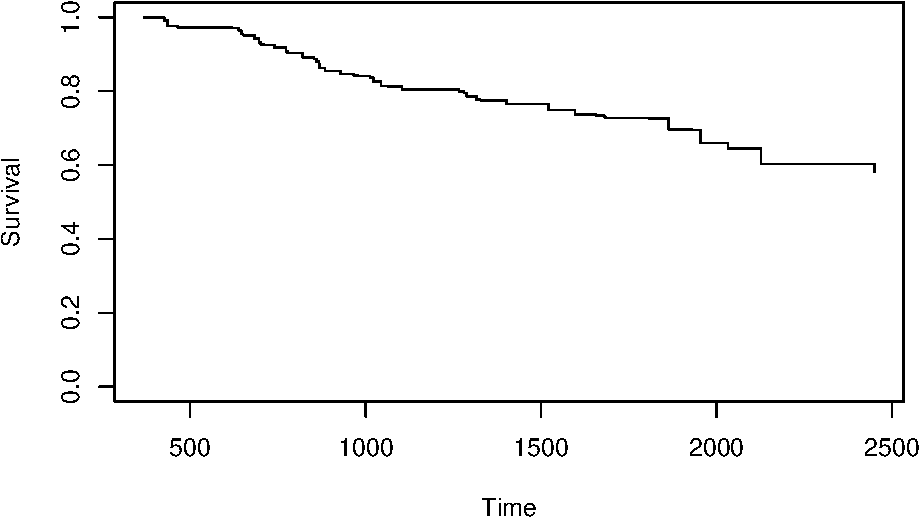
\includegraphics{bookdown_files/figure-latex/unnamed-chunk-69-1.pdf}

\BeginKnitrBlock{rmdhint_sestelo}
The \textbf{inclusion of continuous covariates} can be computationally
demanding. In particular, the use of bootstrap resampling techniques are
time-consuming processes because it is necessary to estimate the model a
great number of times.
\EndKnitrBlock{rmdhint_sestelo}

The use of the \texttt{condSURV} package to more than two consecutive
events is illustrated in the Appendix of
\citet{meiramachado-sestelo:2016}.

\appendix


\chapter{\texorpdfstring{Installation of \texttt{R} and
\texttt{RStudio}}{Installation of R and RStudio}}\label{appendix-install}

You can follow these steps to install \texttt{R} and \texttt{Rstudio},
please note that there will be a few new releases of \texttt{R} every
year, and you may want to upgrade \texttt{R} occasionally.

\begin{itemize}
\item
  For \textbf{Ubuntu} users, kindly follow the corresponding
  instructions
  \href{https://www.digitalocean.com/community/tutorials/how-to-install-r-on-ubuntu-16-04-2}{here}.
\item
  For \textbf{Mac OS X} users download \texttt{R} from
  \href{https://cran.r-project.org}{here} or from the url below. To this
  end, click on \emph{Download R for Mac OS X}. Then click on
  \emph{Download R-3.4.2.pkg} (or a newer version) and install it. Leave
  all default settings in the installation options. Optional for some
  graphic experiences, download and install
  \href{http://xquartz.macosforge.org/}{\texttt{XQuartz}}.
\end{itemize}

Once installed \texttt{R}, you can download \texttt{RStudio\ IDE} from
\href{http://www.rstudio.com/ide/download/desktop}{here} or from the url
below. You must choose the appropriate version to your operative system
and hardware (only certain Ubuntu and Fedora versions are supported),
and install it using the package manager.

\chapter{\texorpdfstring{Introduction to
\texttt{RStudio}}{Introduction to RStudio}}\label{appendix-rstudio}

\href{https://www.rstudio.com}{\texttt{RStudio}} is the premier
integrated development environment (IDE) for \texttt{R}. It is available
in open source and commercial editions on the desktop (Windows, Mac, and
Linux) and from a web browser to a Linux server running RStudio Server
or RStudio Server Pro.

You can find a global view of the IDE in this
\href{https://www.rstudio.com/wp-content/uploads/2016/01/rstudio-IDE-cheatsheet.pdf}{Cheat
Sheet}.

An important advice is that for running a line or code selection from
the script in the console, you can do it with the keyboard shortcut
\texttt{\textquotesingle{}Ctrl+Enter\textquotesingle{}} (Linux) or
\texttt{\textquotesingle{}Cmd+Enter\textquotesingle{}} (Mac OS X).

\chapter{\texorpdfstring{Introduction to
\texttt{R}}{Introduction to R}}\label{appendix-r}

The manual
\href{https://cran.r-project.org/doc/manuals/r-release/R-intro.html}{``An
Introduction to R''} gives an introduction to the language and how to
use \texttt{R} for doing statistical analysis and graphcis in detail.

Additionally, in this section you can find a set of Cheat Sheets of this
programming language:

\begin{itemize}
\item
  \href{https://www.rstudio.com/wp-content/uploads/2016/10/r-cheat-sheet-3.pdf}{R
  Base} for first steps and basic functions of the language.
\item
  \href{https://www.rstudio.com/wp-content/uploads/2016/02/advancedR.pdf}{R
  Advanced} for environments, data structures, functions, subsetting and
  more advanced things.
\item
  The
  \href{https://github.com/rstudio/cheatsheets/raw/master/data-import.pdf}{Data
  Import} cheat sheet reminds you how to read in flat files with
  \url{http://readr.tidyverse.org/}, work with the results as tibbles,
  and reshape messy data with the
  \href{https://cran.r-project.org/web/packages/tidyr/index.html}{\texttt{tidyr}}
  package. Use \texttt{tidyr} to reshape your tables into tidy data, the
  data format that works the most seamlessly with \texttt{R} and the
  \href{https://cran.r-project.org/web/packages/tidyverse/index.html}{\texttt{tidyverse}}.
\item
  \href{https://github.com/rstudio/cheatsheets/raw/master/data-transformation.pdf}{Data
  Transformations} for some functions in
  \href{https://cran.r-project.org/web/packages/dplyr/index.html}{\texttt{dplyr}}
  packages very useful and computational efficient to preprocess data.
\item
  \href{https://github.com/rstudio/cheatsheets/raw/master/data-visualization-2.1.pdf}{Data
  Visualization} for make beautiful and customizable plots of your data
  by means of the
  \href{https://cran.r-project.org/web/packages/ggplot2/index.html}{\texttt{ggplot2}}
  package. It implements the grammar of graphics, an easy to use system
  for building plots.
\end{itemize}

Finally, you can find below a list with some well-know \textbf{web
resources} related with this statistical language:

\begin{itemize}
\tightlist
\item
  \href{https://www.r-bloggers.com}{R-bloggers}
\item
  \href{http://www.statmethods.net/index.html}{Quick-R site}
\item
  \href{http://revolution-computing.typepad.com}{Revolutions}
\item
  \href{http://journal.r-project.org/current.html}{The R Journal}
\item
  \href{https://www.jstatsoft.org/index}{Journal of Statistical
  Software}
\end{itemize}

\bibliography{bib/bib_condsurv.bib,bib/bibliografia.bib}

\backmatter
\printindex


\end{document}
